\subsection{Diagrammi di classi}
I diagrammi di classi rappresentano il sistema della rubrica con le funzionalità di gestione dei contatti, dei tag, importazione/esportazione di dati, configurazioni e salvataggio dei dati in locale o su DB.
\begin{itemize}[noitemsep, topsep=5pt]
	\item \textbf{Contact}: Modella un contatto con attributi come nome, cognome, numeri di telefono, e-mail, immagine del profilo, e tag associati. Ha metodi per gestire i contatti, aggiungere e rimuovere numeri e e-mail, e per gestire i tag associati.
	\item \textbf{Tag}: Modella un'etichetta associata ai contatti, con attributi come id, descrizione, e un indice statico. Include metodi per ottenere e impostare descrizioni e id, e per confrontare gli oggetti.
	\item \textbf{AddressBook}: Contiene contatti e tag. È una classe singleton, quindi ha un'istanza unica, e gestisce il salvataggio dei dati tramite un database o la serializzazione. Ha metodi per aggiungere, rimuovere e ottenere contatti e tag, e per caricare e salvare i dati.
	\item \textbf{MainController}: Gestisce l'interfaccia utente principale, con metodi per inizializzare i componenti dell'interfaccia, aggiungere, modificare, rimuovere contatti, per visualizzare pop-up per l'importazione/esportazione e la gestione dei tag.
	\item \textbf{ImportPopupController}, \textbf{ExportPopupController}, \textbf{ManageTagsPopupController}, \textbf{ConfigPopupController}, \textbf{ImagePopupController}: Gestiscono i pop-up per importare/esportare contatti, gestire i tag, gestire la configurazione (link del DB) e gestire le immagini di profilo.
	\item \textbf{ConfirmPopupController}: Gestisce anch'essa un pop-up di conferma di un'eventuale operazione di eliminazione di un contatto o di un tag richiesta dall'utente.
	\item \textbf{Database}: Gestisce l'interazione con un database MongoDB per l'archiviazione di contatti e tag. Ha metodi per inserire, aggiornare, rimuovere, recuperare contatti e tag dal database.
\end{itemize}

\subsubsection{Livello di dettaglio basso}
% generated by Plantuml 1.2024.3       
\definecolor{plantucolor0000}{RGB}{241,241,241}
\definecolor{plantucolor0001}{RGB}{24,24,24}
\definecolor{plantucolor0002}{RGB}{173,209,178}
\definecolor{plantucolor0003}{RGB}{0,0,0}
\definecolor{plantucolor0004}{RGB}{200,41,48}
\definecolor{plantucolor0005}{RGB}{132,190,132}
\definecolor{plantucolor0006}{RGB}{3,128,72}
\definecolor{plantucolor0007}{RGB}{242,77,92}
\definecolor{plantucolor0008}{RGB}{180,167,229}

\begin{adjustbox}{width=.9\paperwidth, center}
\resizebox{\textwidth}{!}{
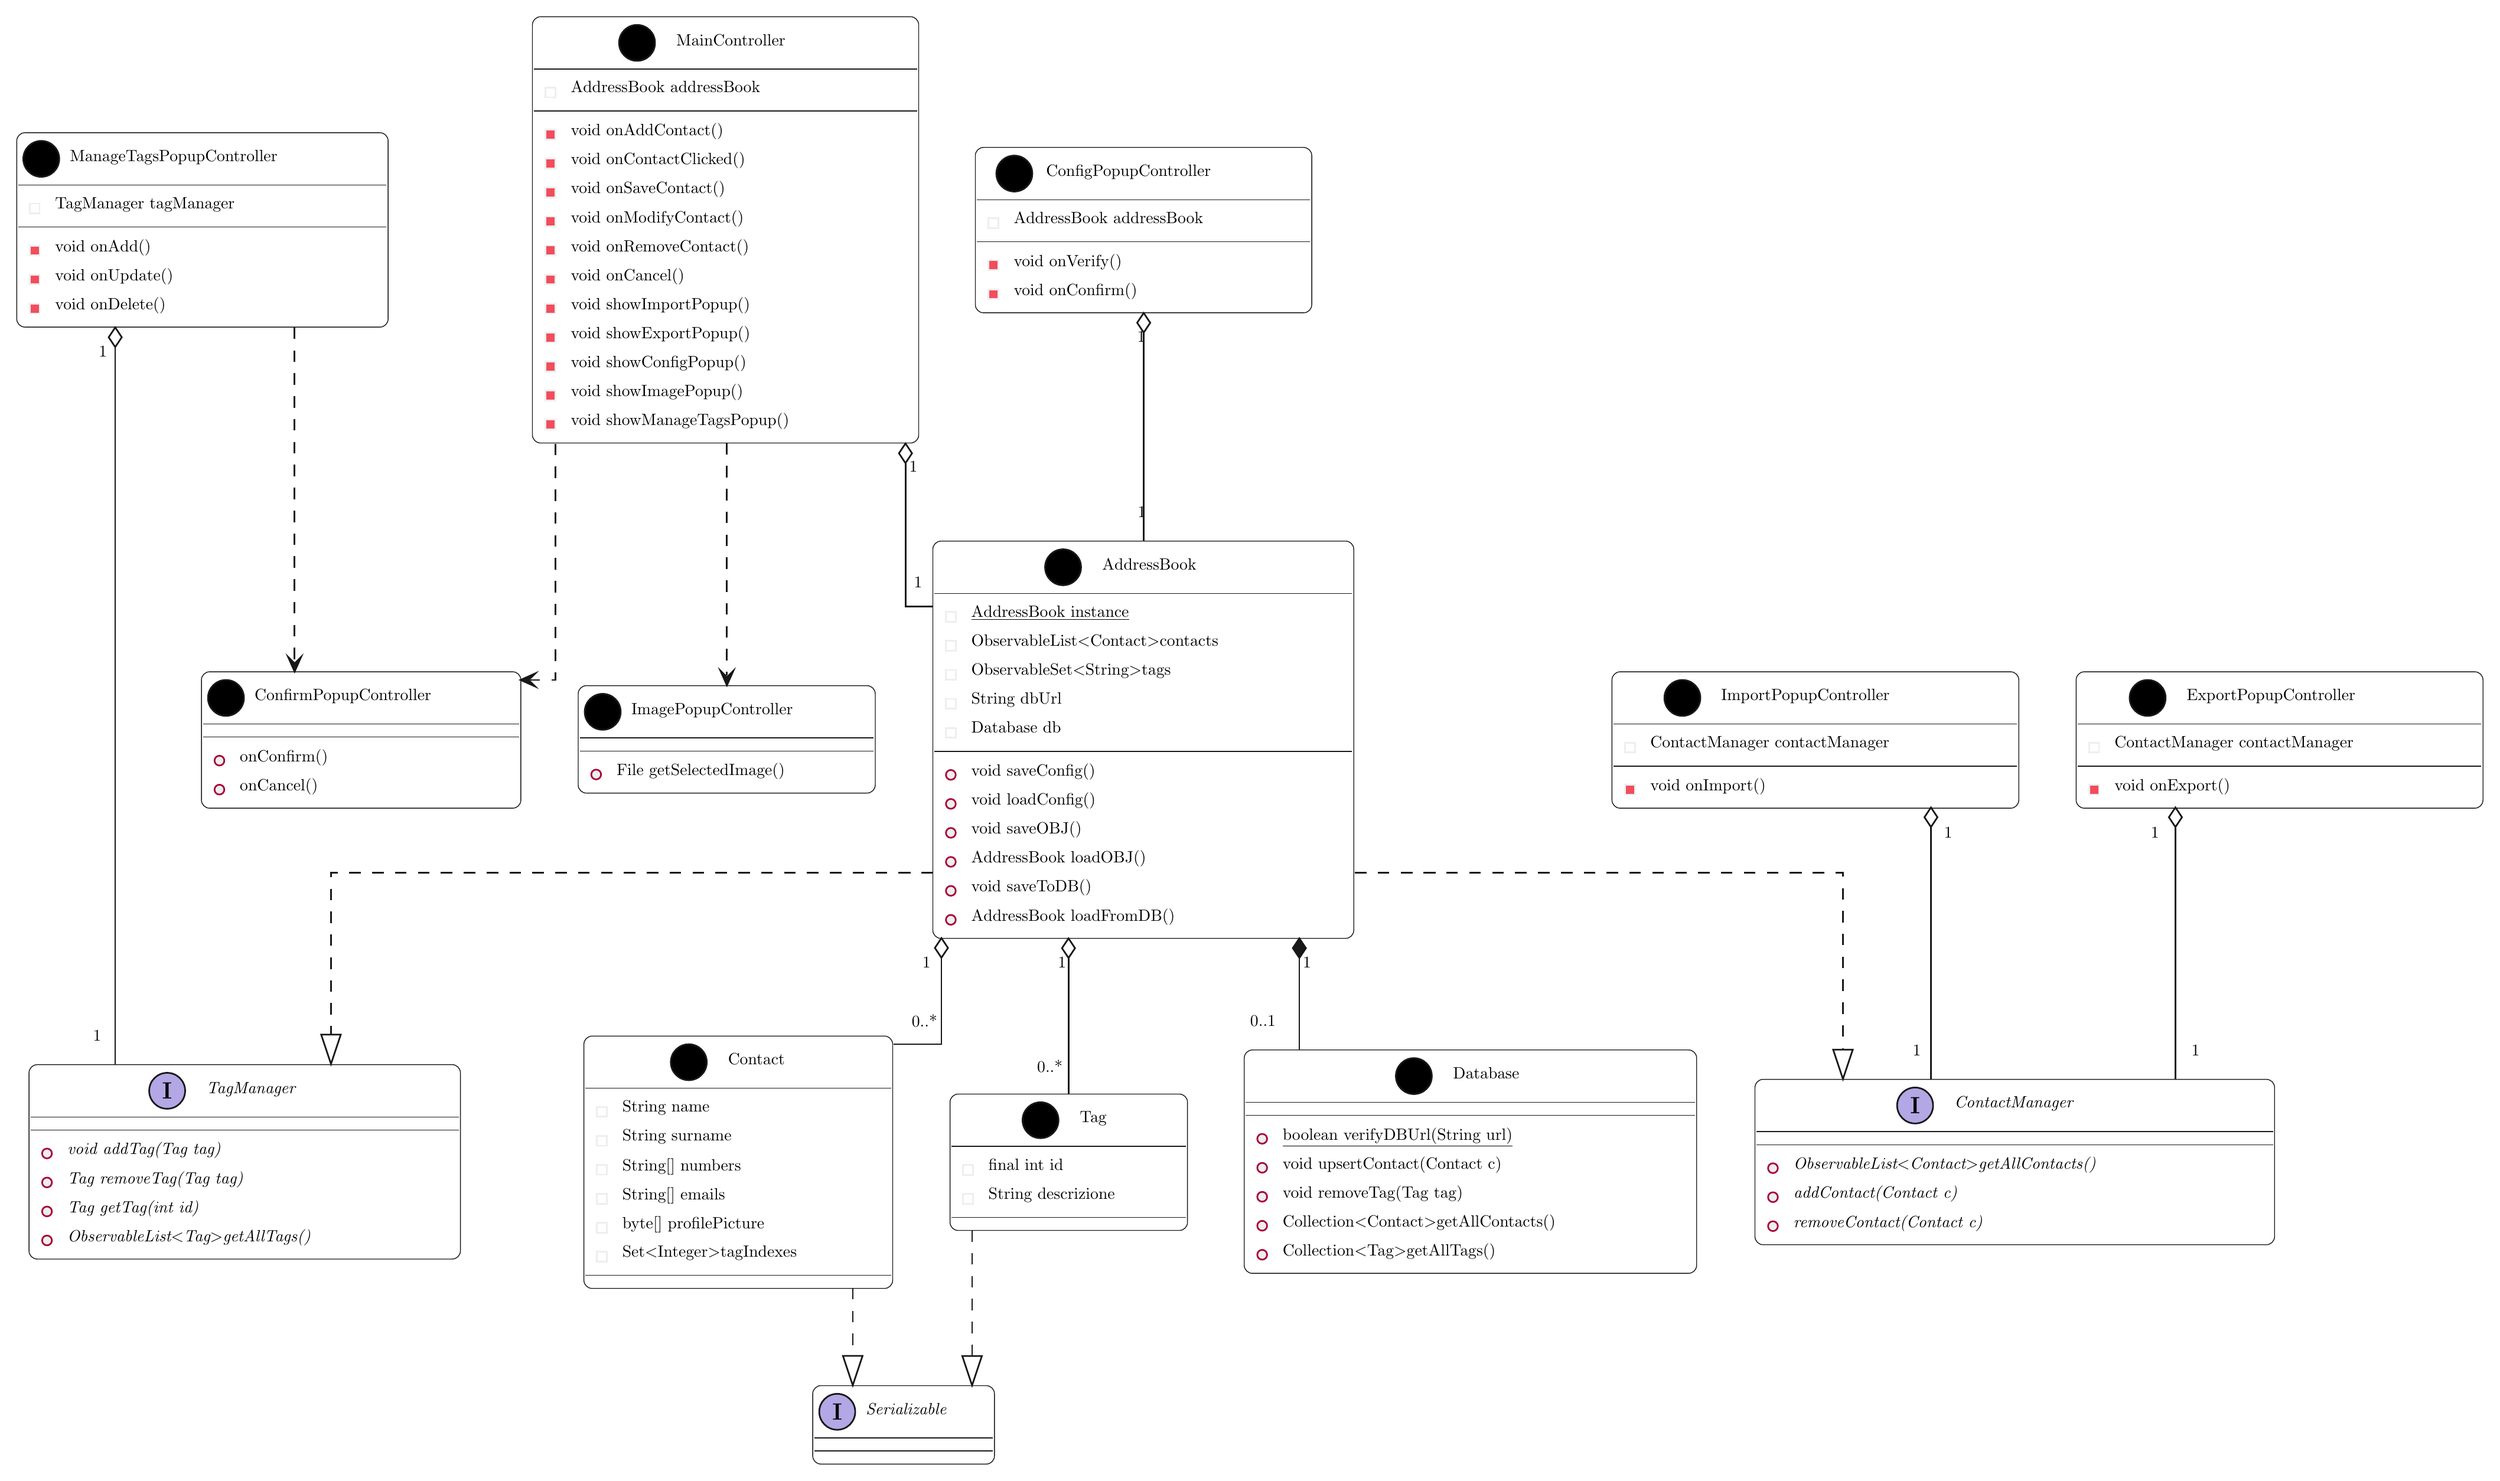
\begin{tikzpicture}[yscale=-1
,pstyle0/.style={color=plantucolor0001,fill=plantucolor0000,line width=0.5pt}
,pstyle1/.style={color=plantucolor0001,fill=plantucolor0002,line width=1.0pt}
,pstyle2/.style={color=plantucolor0001,line width=0.5pt}
,pstyle3/.style={color=plantucolor0004,line width=1.0pt}
,pstyle4/.style={color=plantucolor0006,fill=plantucolor0005,line width=1.0pt}
,pstyle5/.style={color=plantucolor0004,fill=plantucolor0007,line width=1.0pt}
,pstyle6/.style={color=plantucolor0001,fill=plantucolor0008,line width=1.0pt}
,pstyle7/.style={color=plantucolor0001,line width=1.0pt,dash pattern=on 7.0pt off 7.0pt}
,pstyle8/.style={color=plantucolor0001,line width=1.0pt}
,pstyle9/.style={color=plantucolor0001,fill=plantucolor0001,line width=1.0pt}
]
\draw[pstyle0] (354pt,636pt) arc (180:270:5pt) -- (359pt,631pt) -- (537.9151pt,631pt) arc (270:360:5pt) -- (542.9151pt,636pt) -- (542.9151pt,780.4766pt) arc (0:90:5pt) -- (537.9151pt,785.4766pt) -- (359pt,785.4766pt) arc (90:180:5pt) -- (354pt,780.4766pt) -- cycle;
\draw[pstyle1] (418.1712pt,647pt) ellipse (11pt and 11pt);
\node at (418.1712pt,647pt)[]{\textbf{\Large C}};
\node at (438.6712pt,638.127pt)[below right,color=black]{Contact};
\draw[pstyle2] (355pt,663pt) -- (541.9151pt,663pt);
\draw[pstyle3] (362pt,674.373pt) rectangle (368pt,680.373pt);
\node at (374pt,667pt)[below right,color=black]{String name};
\draw[pstyle3] (362pt,692.1191pt) rectangle (368pt,698.1191pt);
\node at (374pt,684.7461pt)[below right,color=black]{String surname};
\draw[pstyle3] (362pt,709.8652pt) rectangle (368pt,715.8652pt);
\node at (374pt,702.4922pt)[below right,color=black]{String[] numbers};
\draw[pstyle3] (362pt,727.6113pt) rectangle (368pt,733.6113pt);
\node at (374pt,720.2383pt)[below right,color=black]{String[] emails};
\draw[pstyle3] (362pt,745.3574pt) rectangle (368pt,751.3574pt);
\node at (374pt,737.9844pt)[below right,color=black]{byte[] profilePicture};
\draw[pstyle3] (362pt,763.1035pt) rectangle (368pt,769.1035pt);
\node at (374pt,755.7305pt)[below right,color=black]{Set\textless Integer\textgreater  tagIndexes};
\draw[pstyle2] (355pt,777.4766pt) -- (541.9151pt,777.4766pt);
\draw[pstyle0] (567.5pt,333pt) arc (180:270:5pt) -- (572.5pt,328pt) -- (820.0265pt,328pt) arc (270:360:5pt) -- (825.0265pt,333pt) -- (825.0265pt,566.207pt) arc (0:90:5pt) -- (820.0265pt,571.207pt) -- (572.5pt,571.207pt) arc (90:180:5pt) -- (567.5pt,566.207pt) -- cycle;
\draw[pstyle1] (647.1733pt,344pt) ellipse (11pt and 11pt);
\node at (647.1733pt,344pt)[]{\textbf{\Large C}};
\node at (667.6733pt,335.127pt)[below right,color=black]{AddressBook};
\draw[pstyle2] (568.5pt,360pt) -- (824.0265pt,360pt);
\draw[pstyle3] (575.5pt,371.373pt) rectangle (581.5pt,377.373pt);
\node at (587.5pt,364pt)[below right,color=black]{\underline{AddressBook instance}};
\draw[pstyle3] (575.5pt,389.1191pt) rectangle (581.5pt,395.1191pt);
\node at (587.5pt,381.7461pt)[below right,color=black]{ObservableList\textless Contact\textgreater  contacts};
\draw[pstyle3] (575.5pt,406.8652pt) rectangle (581.5pt,412.8652pt);
\node at (587.5pt,399.4922pt)[below right,color=black]{ObservableSet\textless String\textgreater  tags};
\draw[pstyle3] (575.5pt,424.6113pt) rectangle (581.5pt,430.6113pt);
\node at (587.5pt,417.2383pt)[below right,color=black]{String dbUrl};
\draw[pstyle3] (575.5pt,442.3574pt) rectangle (581.5pt,448.3574pt);
\node at (587.5pt,434.9844pt)[below right,color=black]{Database db};
\draw[pstyle2] (568.5pt,456.7305pt) -- (824.0265pt,456.7305pt);
\draw[pstyle4] (578.5pt,471.1035pt) ellipse (3pt and 3pt);
\node at (587.5pt,460.7305pt)[below right,color=black]{void saveConfig()};
\draw[pstyle4] (578.5pt,488.8496pt) ellipse (3pt and 3pt);
\node at (587.5pt,478.4766pt)[below right,color=black]{void loadConfig()};
\draw[pstyle4] (578.5pt,506.5957pt) ellipse (3pt and 3pt);
\node at (587.5pt,496.2227pt)[below right,color=black]{void saveOBJ()};
\draw[pstyle4] (578.5pt,524.3418pt) ellipse (3pt and 3pt);
\node at (587.5pt,513.9688pt)[below right,color=black]{AddressBook loadOBJ()};
\draw[pstyle4] (578.5pt,542.0879pt) ellipse (3pt and 3pt);
\node at (587.5pt,531.7148pt)[below right,color=black]{void saveToDB()};
\draw[pstyle4] (578.5pt,559.834pt) ellipse (3pt and 3pt);
\node at (587.5pt,549.4609pt)[below right,color=black]{AddressBook loadFromDB()};
\draw[pstyle0] (322.5pt,12pt) arc (180:270:5pt) -- (327.5pt,7pt) -- (553.8435pt,7pt) arc (270:360:5pt) -- (558.8435pt,12pt) -- (558.8435pt,262.9531pt) arc (0:90:5pt) -- (553.8435pt,267.9531pt) -- (327.5pt,267.9531pt) arc (90:180:5pt) -- (322.5pt,262.9531pt) -- cycle;
\draw[pstyle1] (386.5218pt,23pt) ellipse (11pt and 11pt);
\node at (386.5218pt,23pt)[]{\textbf{\Large C}};
\node at (407.0218pt,14.127pt)[below right,color=black]{MainController};
\draw[pstyle2] (323.5pt,39pt) -- (557.8435pt,39pt);
\draw[pstyle3] (330.5pt,50.373pt) rectangle (336.5pt,56.373pt);
\node at (342.5pt,43pt)[below right,color=black]{AddressBook addressBook};
\draw[pstyle2] (323.5pt,64.7461pt) -- (557.8435pt,64.7461pt);
\draw[pstyle5] (330.5pt,76.1191pt) rectangle (336.5pt,82.1191pt);
\node at (342.5pt,68.7461pt)[below right,color=black]{void onAddContact()};
\draw[pstyle5] (330.5pt,93.8652pt) rectangle (336.5pt,99.8652pt);
\node at (342.5pt,86.4922pt)[below right,color=black]{void onContactClicked()};
\draw[pstyle5] (330.5pt,111.6113pt) rectangle (336.5pt,117.6113pt);
\node at (342.5pt,104.2383pt)[below right,color=black]{void onSaveContact()};
\draw[pstyle5] (330.5pt,129.3574pt) rectangle (336.5pt,135.3574pt);
\node at (342.5pt,121.9844pt)[below right,color=black]{void onModifyContact()};
\draw[pstyle5] (330.5pt,147.1035pt) rectangle (336.5pt,153.1035pt);
\node at (342.5pt,139.7305pt)[below right,color=black]{void onRemoveContact()};
\draw[pstyle5] (330.5pt,164.8496pt) rectangle (336.5pt,170.8496pt);
\node at (342.5pt,157.4766pt)[below right,color=black]{void onCancel()};
\draw[pstyle5] (330.5pt,182.5957pt) rectangle (336.5pt,188.5957pt);
\node at (342.5pt,175.2227pt)[below right,color=black]{void showImportPopup()};
\draw[pstyle5] (330.5pt,200.3418pt) rectangle (336.5pt,206.3418pt);
\node at (342.5pt,192.9688pt)[below right,color=black]{void showExportPopup()};
\draw[pstyle5] (330.5pt,218.0879pt) rectangle (336.5pt,224.0879pt);
\node at (342.5pt,210.7148pt)[below right,color=black]{void showConfigPopup()};
\draw[pstyle5] (330.5pt,235.834pt) rectangle (336.5pt,241.834pt);
\node at (342.5pt,228.4609pt)[below right,color=black]{void showImagePopup()};
\draw[pstyle5] (330.5pt,253.5801pt) rectangle (336.5pt,259.5801pt);
\node at (342.5pt,246.207pt)[below right,color=black]{void showManageTagsPopup()};
\draw[pstyle0] (983pt,413pt) arc (180:270:5pt) -- (988pt,408pt) -- (1226.9191pt,408pt) arc (270:360:5pt) -- (1231.9191pt,413pt) -- (1231.9191pt,486.4922pt) arc (0:90:5pt) -- (1226.9191pt,491.4922pt) -- (988pt,491.4922pt) arc (90:180:5pt) -- (983pt,486.4922pt) -- cycle;
\draw[pstyle1] (1026.0828pt,424pt) ellipse (11pt and 11pt);
\node at (1026.0828pt,424pt)[]{\textbf{\Large C}};
\node at (1046.3234pt,415.127pt)[below right,color=black]{ImportPopupController};
\draw[pstyle2] (984pt,440pt) -- (1230.9191pt,440pt);
\draw[pstyle3] (991pt,451.373pt) rectangle (997pt,457.373pt);
\node at (1003pt,444pt)[below right,color=black]{ContactManager contactManager};
\draw[pstyle2] (984pt,465.7461pt) -- (1230.9191pt,465.7461pt);
\draw[pstyle5] (991pt,477.1191pt) rectangle (997pt,483.1191pt);
\node at (1003pt,469.7461pt)[below right,color=black]{void onImport()};
\draw[pstyle0] (1267pt,413pt) arc (180:270:5pt) -- (1272pt,408pt) -- (1510.9191pt,408pt) arc (270:360:5pt) -- (1515.9191pt,413pt) -- (1515.9191pt,486.4922pt) arc (0:90:5pt) -- (1510.9191pt,491.4922pt) -- (1272pt,491.4922pt) arc (90:180:5pt) -- (1267pt,486.4922pt) -- cycle;
\draw[pstyle1] (1310.7428pt,424pt) ellipse (11pt and 11pt);
\node at (1310.7428pt,424pt)[]{\textbf{\Large C}};
\node at (1331.1301pt,415.127pt)[below right,color=black]{ExportPopupController};
\draw[pstyle2] (1268pt,440pt) -- (1514.9191pt,440pt);
\draw[pstyle3] (1275pt,451.373pt) rectangle (1281pt,457.373pt);
\node at (1287pt,444pt)[below right,color=black]{ContactManager contactManager};
\draw[pstyle2] (1268pt,465.7461pt) -- (1514.9191pt,465.7461pt);
\draw[pstyle5] (1275pt,477.1191pt) rectangle (1281pt,483.1191pt);
\node at (1287pt,469.7461pt)[below right,color=black]{void onExport()};
\draw[pstyle0] (7pt,83pt) arc (180:270:5pt) -- (12pt,78pt) -- (229.2146pt,78pt) arc (270:360:5pt) -- (234.2146pt,83pt) -- (234.2146pt,191.9844pt) arc (0:90:5pt) -- (229.2146pt,196.9844pt) -- (12pt,196.9844pt) arc (90:180:5pt) -- (7pt,191.9844pt) -- cycle;
\draw[pstyle1] (22pt,94pt) ellipse (11pt and 11pt);
\node at (22pt,94pt)[]{\textbf{\Large C}};
\node at (36pt,85.127pt)[below right,color=black]{ManageTagsPopupController};
\draw[pstyle2] (8pt,110pt) -- (233.2146pt,110pt);
\draw[pstyle3] (15pt,121.373pt) rectangle (21pt,127.373pt);
\node at (27pt,114pt)[below right,color=black]{TagManager tagManager};
\draw[pstyle2] (8pt,135.7461pt) -- (233.2146pt,135.7461pt);
\draw[pstyle5] (15pt,147.1191pt) rectangle (21pt,153.1191pt);
\node at (27pt,139.7461pt)[below right,color=black]{void onAdd()};
\draw[pstyle5] (15pt,164.8652pt) rectangle (21pt,170.8652pt);
\node at (27pt,157.4922pt)[below right,color=black]{void onUpdate()};
\draw[pstyle5] (15pt,182.6113pt) rectangle (21pt,188.6113pt);
\node at (27pt,175.2383pt)[below right,color=black]{void onDelete()};
\draw[pstyle0] (350.5pt,421.5pt) arc (180:270:5pt) -- (355.5pt,416.5pt) -- (527.2543pt,416.5pt) arc (270:360:5pt) -- (532.2543pt,421.5pt) -- (532.2543pt,477.2461pt) arc (0:90:5pt) -- (527.2543pt,482.2461pt) -- (355.5pt,482.2461pt) arc (90:180:5pt) -- (350.5pt,477.2461pt) -- cycle;
\draw[pstyle1] (365.5pt,432.5pt) ellipse (11pt and 11pt);
\node at (365.5pt,432.5pt)[]{\textbf{\Large C}};
\node at (379.5pt,423.627pt)[below right,color=black]{ImagePopupController};
\draw[pstyle2] (351.5pt,448.5pt) -- (531.2543pt,448.5pt);
\draw[pstyle2] (351.5pt,456.5pt) -- (531.2543pt,456.5pt);
\draw[pstyle4] (361.5pt,470.873pt) ellipse (3pt and 3pt);
\node at (370.5pt,460.5pt)[below right,color=black]{File getSelectedImage()};
\draw[pstyle0] (120pt,413pt) arc (180:270:5pt) -- (125pt,408pt) -- (310.4331pt,408pt) arc (270:360:5pt) -- (315.4331pt,413pt) -- (315.4331pt,486.4922pt) arc (0:90:5pt) -- (310.4331pt,491.4922pt) -- (125pt,491.4922pt) arc (90:180:5pt) -- (120pt,486.4922pt) -- cycle;
\draw[pstyle1] (135pt,424pt) ellipse (11pt and 11pt);
\node at (135pt,424pt)[]{\textbf{\Large C}};
\node at (149pt,415.127pt)[below right,color=black]{ConfirmPopupController};
\draw[pstyle2] (121pt,440pt) -- (314.4331pt,440pt);
\draw[pstyle2] (121pt,448pt) -- (314.4331pt,448pt);
\draw[pstyle4] (131pt,462.373pt) ellipse (3pt and 3pt);
\node at (140pt,452pt)[below right,color=black]{onConfirm()};
\draw[pstyle4] (131pt,480.1191pt) ellipse (3pt and 3pt);
\node at (140pt,469.7461pt)[below right,color=black]{onCancel()};
\draw[pstyle0] (593.5pt,92pt) arc (180:270:5pt) -- (598.5pt,87pt) -- (794.3225pt,87pt) arc (270:360:5pt) -- (799.3225pt,92pt) -- (799.3225pt,183.2383pt) arc (0:90:5pt) -- (794.3225pt,188.2383pt) -- (598.5pt,188.2383pt) arc (90:180:5pt) -- (593.5pt,183.2383pt) -- cycle;
\draw[pstyle1] (617.3509pt,103pt) ellipse (11pt and 11pt);
\node at (617.3509pt,103pt)[]{\textbf{\Large C}};
\node at (633.3178pt,94.127pt)[below right,color=black]{ConfigPopupController};
\draw[pstyle2] (594.5pt,119pt) -- (798.3225pt,119pt);
\draw[pstyle3] (601.5pt,130.373pt) rectangle (607.5pt,136.373pt);
\node at (613.5pt,123pt)[below right,color=black]{AddressBook addressBook};
\draw[pstyle2] (594.5pt,144.7461pt) -- (798.3225pt,144.7461pt);
\draw[pstyle5] (601.5pt,156.1191pt) rectangle (607.5pt,162.1191pt);
\node at (613.5pt,148.7461pt)[below right,color=black]{void onVerify()};
\draw[pstyle5] (601.5pt,173.8652pt) rectangle (607.5pt,179.8652pt);
\node at (613.5pt,166.4922pt)[below right,color=black]{void onConfirm()};
\draw[pstyle0] (578pt,671.5pt) arc (180:270:5pt) -- (583pt,666.5pt) -- (718.299pt,666.5pt) arc (270:360:5pt) -- (723.299pt,671.5pt) -- (723.299pt,744.9922pt) arc (0:90:5pt) -- (718.299pt,749.9922pt) -- (583pt,749.9922pt) arc (90:180:5pt) -- (578pt,744.9922pt) -- cycle;
\draw[pstyle1] (633.3813pt,682.5pt) ellipse (11pt and 11pt);
\node at (633.3813pt,682.5pt)[]{\textbf{\Large C}};
\node at (653.8813pt,673.627pt)[below right,color=black]{Tag};
\draw[pstyle2] (579pt,698.5pt) -- (722.299pt,698.5pt);
\draw[pstyle3] (586pt,709.873pt) rectangle (592pt,715.873pt);
\node at (598pt,702.5pt)[below right,color=black]{final int id};
\draw[pstyle3] (586pt,727.6191pt) rectangle (592pt,733.6191pt);
\node at (598pt,720.2461pt)[below right,color=black]{String descrizione};
\draw[pstyle2] (579pt,741.9922pt) -- (722.299pt,741.9922pt);
\draw[pstyle0] (758pt,644.5pt) arc (180:270:5pt) -- (763pt,639.5pt) -- (1029.8151pt,639.5pt) arc (270:360:5pt) -- (1034.8151pt,644.5pt) -- (1034.8151pt,771.2305pt) arc (0:90:5pt) -- (1029.8151pt,776.2305pt) -- (763pt,776.2305pt) arc (90:180:5pt) -- (758pt,771.2305pt) -- cycle;
\draw[pstyle1] (861.7928pt,655.5pt) ellipse (11pt and 11pt);
\node at (861.7928pt,655.5pt)[]{\textbf{\Large C}};
\node at (882.2928pt,646.627pt)[below right,color=black]{Database};
\draw[pstyle2] (759pt,671.5pt) -- (1033.8151pt,671.5pt);
\draw[pstyle2] (759pt,679.5pt) -- (1033.8151pt,679.5pt);
\draw[pstyle4] (769pt,693.873pt) ellipse (3pt and 3pt);
\node at (778pt,683.5pt)[below right,color=black]{\underline{boolean verifyDBUrl(String url)}};
\draw[pstyle4] (769pt,711.6191pt) ellipse (3pt and 3pt);
\node at (778pt,701.2461pt)[below right,color=black]{void upsertContact(Contact c)};
\draw[pstyle4] (769pt,729.3652pt) ellipse (3pt and 3pt);
\node at (778pt,718.9922pt)[below right,color=black]{void removeTag(Tag tag)};
\draw[pstyle4] (769pt,747.1113pt) ellipse (3pt and 3pt);
\node at (778pt,736.7383pt)[below right,color=black]{Collection\textless Contact\textgreater  getAllContacts()};
\draw[pstyle4] (769pt,764.8574pt) ellipse (3pt and 3pt);
\node at (778pt,754.4844pt)[below right,color=black]{Collection\textless Tag\textgreater  getAllTags()};
\draw[pstyle0] (494pt,850pt) arc (180:270:5pt) -- (499pt,845pt) -- (600.2pt,845pt) arc (270:360:5pt) -- (605.2pt,850pt) -- (605.2pt,888pt) arc (0:90:5pt) -- (600.2pt,893pt) -- (499pt,893pt) arc (90:180:5pt) -- (494pt,888pt) -- cycle;
\draw[pstyle6] (509pt,861pt) ellipse (11pt and 11pt);
\node at (509pt,861pt)[]{\textbf{\Large I}};
\node at (523pt,852.127pt)[below right,color=black]{\textit{Serializable}};
\draw[pstyle2] (495pt,877pt) -- (604.2pt,877pt);
\draw[pstyle2] (495pt,885pt) -- (604.2pt,885pt);
\draw[pstyle0] (14.5pt,653.5pt) arc (180:270:5pt) -- (19.5pt,648.5pt) -- (273.4446pt,648.5pt) arc (270:360:5pt) -- (278.4446pt,653.5pt) -- (278.4446pt,762.4844pt) arc (0:90:5pt) -- (273.4446pt,767.4844pt) -- (19.5pt,767.4844pt) arc (90:180:5pt) -- (14.5pt,762.4844pt) -- cycle;
\draw[pstyle6] (99.025pt,664.5pt) ellipse (11pt and 11pt);
\node at (99.025pt,664.5pt)[]{\textbf{\Large I}};
\node at (119.525pt,655.627pt)[below right,color=black]{\textit{TagManager}};
\draw[pstyle2] (15.5pt,680.5pt) -- (277.4446pt,680.5pt);
\draw[pstyle2] (15.5pt,688.5pt) -- (277.4446pt,688.5pt);
\draw[pstyle4] (25.5pt,702.873pt) ellipse (3pt and 3pt);
\node at (34.5pt,692.5pt)[below right,color=black]{\textit{void addTag(Tag tag)}};
\draw[pstyle4] (25.5pt,720.6191pt) ellipse (3pt and 3pt);
\node at (34.5pt,710.2461pt)[below right,color=black]{\textit{Tag removeTag(Tag tag)}};
\draw[pstyle4] (25.5pt,738.3652pt) ellipse (3pt and 3pt);
\node at (34.5pt,727.9922pt)[below right,color=black]{\textit{Tag getTag(int id)}};
\draw[pstyle4] (25.5pt,756.1113pt) ellipse (3pt and 3pt);
\node at (34.5pt,745.7383pt)[below right,color=black]{\textit{ObservableList\textless Tag\textgreater  getAllTags()}};
\draw[pstyle0] (1070.5pt,662.5pt) arc (180:270:5pt) -- (1075.5pt,657.5pt) -- (1383.3992pt,657.5pt) arc (270:360:5pt) -- (1388.3992pt,662.5pt) -- (1388.3992pt,753.7383pt) arc (0:90:5pt) -- (1383.3992pt,758.7383pt) -- (1075.5pt,758.7383pt) arc (90:180:5pt) -- (1070.5pt,753.7383pt) -- cycle;
\draw[pstyle6] (1168.4733pt,673.5pt) ellipse (11pt and 11pt);
\node at (1168.4733pt,673.5pt)[]{\textbf{\Large I}};
\node at (1188.9733pt,664.627pt)[below right,color=black]{\textit{ContactManager}};
\draw[pstyle2] (1071.5pt,689.5pt) -- (1387.3992pt,689.5pt);
\draw[pstyle2] (1071.5pt,697.5pt) -- (1387.3992pt,697.5pt);
\draw[pstyle4] (1081.5pt,711.873pt) ellipse (3pt and 3pt);
\node at (1090.5pt,701.5pt)[below right,color=black]{\textit{ObservableList\textless Contact\textgreater  getAllContacts()}};
\draw[pstyle4] (1081.5pt,729.6191pt) ellipse (3pt and 3pt);
\node at (1090.5pt,719.2461pt)[below right,color=black]{\textit{addContact(Contact c)}};
\draw[pstyle4] (1081.5pt,747.3652pt) ellipse (3pt and 3pt);
\node at (1090.5pt,736.9922pt)[below right,color=black]{\textit{removeContact(Contact c)}};
\draw[pstyle7] (518.5pt,785.2pt) ..controls (518.5pt,806.83pt) and (518.5pt,810.77pt) .. (518.5pt,826.78pt);
\draw[pstyle8] (518.5pt,844.78pt) -- (524.5pt,826.78pt) -- (512.5pt,826.78pt) -- (518.5pt,844.78pt) -- cycle;
\draw[pstyle7] (591.5pt,749.88pt) ..controls (591.5pt,780.07pt) and (591.5pt,801.75pt) .. (591.5pt,826.82pt);
\draw[pstyle8] (591.5pt,844.82pt) -- (597.5pt,826.82pt) -- (585.5pt,826.82pt) -- (591.5pt,844.82pt) -- cycle;
\draw[pstyle8] (572.75pt,583.03pt) ..controls (572.75pt,618.54pt) and (572.75pt,636pt) .. (572.75pt,636pt) ..controls (572.75pt,636pt) and (560.31pt,636pt) .. (543.3pt,636pt);
\draw[pstyle8] (572.75pt,571.03pt) -- (568.75pt,577.03pt) -- (572.75pt,583.03pt) -- (576.75pt,577.03pt) -- (572.75pt,571.03pt) -- cycle;
\node at (557.6196pt,579.3367pt)[below right,color=black]{1};
\node at (551.0713pt,614.1251pt)[below right,color=black]{0..*};
\draw[pstyle8] (791.75pt,583.18pt) ..controls (791.75pt,606.62pt) and (791.75pt,618.39pt) .. (791.75pt,639.4pt);
\draw[pstyle9] (791.75pt,571.18pt) -- (787.75pt,577.18pt) -- (791.75pt,583.18pt) -- (795.75pt,577.18pt) -- (791.75pt,571.18pt) -- cycle;
\node at (790.3615pt,579.0906pt)[below right,color=black]{1};
\node at (758.1875pt,615.0628pt)[below right,color=black]{0..1};
\draw[pstyle8] (650.5pt,583.18pt) ..controls (650.5pt,617.36pt) and (650.5pt,640.25pt) .. (650.5pt,666.24pt);
\draw[pstyle8] (650.5pt,571.18pt) -- (646.5pt,577.18pt) -- (650.5pt,583.18pt) -- (654.5pt,577.18pt) -- (650.5pt,571.18pt) -- cycle;
\node at (640.5041pt,579.0906pt)[below right,color=black]{1};
\node at (627.8155pt,641.9974pt)[below right,color=black]{0..*};
\draw[pstyle7] (567.48pt,531pt) ..controls (420.14pt,531pt) and (199.25pt,531pt) .. (199.25pt,531pt) ..controls (199.25pt,531pt) and (199.25pt,578.73pt) .. (199.25pt,630.08pt);
\draw[pstyle8] (199.25pt,648.08pt) -- (205.25pt,630.08pt) -- (193.25pt,630.08pt) -- (199.25pt,648.08pt) -- cycle;
\draw[pstyle7] (825.73pt,531pt) ..controls (951.68pt,531pt) and (1124.33pt,531pt) .. (1124.33pt,531pt) ..controls (1124.33pt,531pt) and (1124.33pt,586.98pt) .. (1124.33pt,639.28pt);
\draw[pstyle8] (1124.33pt,657.28pt) -- (1130.33pt,639.28pt) -- (1118.33pt,639.28pt) -- (1124.33pt,657.28pt) -- cycle;
\draw[pstyle8] (550.75pt,280.24pt) ..controls (550.75pt,332.26pt) and (550.75pt,368pt) .. (550.75pt,368pt) ..controls (550.75pt,368pt) and (557.24pt,368pt) .. (567.47pt,368pt);
\draw[pstyle8] (550.75pt,268.24pt) -- (546.75pt,274.24pt) -- (550.75pt,280.24pt) -- (554.75pt,274.24pt) -- (550.75pt,268.24pt) -- cycle;
\node at (549.584pt,275.8417pt)[below right,color=black]{1};
\node at (552.4145pt,346.5544pt)[below right,color=black]{1};
\draw[pstyle7] (441.5pt,268.01pt) ..controls (441.5pt,322.28pt) and (441.5pt,374.78pt) .. (441.5pt,410.27pt);
\draw[pstyle9] (441.5pt,416.27pt) -- (445.5pt,407.27pt) -- (441.5pt,411.27pt) -- (437.5pt,407.27pt) -- (441.5pt,416.27pt) -- cycle;
\draw[pstyle7] (336.5pt,268.39pt) ..controls (336.5pt,339.48pt) and (336.5pt,413pt) .. (336.5pt,413pt) ..controls (336.5pt,413pt) and (333.85pt,413pt) .. (321.23pt,413pt);
\draw[pstyle9] (315.23pt,413pt) -- (324.23pt,417pt) -- (320.23pt,413pt) -- (324.23pt,409pt) -- (315.23pt,413pt) -- cycle;
\draw[pstyle7] (177pt,197.29pt) ..controls (177pt,259.04pt) and (177pt,347.79pt) .. (177pt,401.87pt);
\draw[pstyle9] (177pt,407.87pt) -- (181pt,398.87pt) -- (177pt,402.87pt) -- (173pt,398.87pt) -- (177pt,407.87pt) -- cycle;
\draw[pstyle8] (1327.75pt,503.03pt) ..controls (1327.75pt,548.27pt) and (1327.75pt,608.67pt) .. (1327.75pt,657.24pt);
\draw[pstyle8] (1327.75pt,491.03pt) -- (1323.75pt,497.03pt) -- (1327.75pt,503.03pt) -- (1331.75pt,497.03pt) -- (1327.75pt,491.03pt) -- cycle;
\node at (1309.2155pt,499.5418pt)[below right,color=black]{1};
\node at (1334.0954pt,632.9938pt)[below right,color=black]{1};
\draw[pstyle8] (1178.17pt,503.03pt) ..controls (1178.17pt,548.27pt) and (1178.17pt,608.67pt) .. (1178.17pt,657.24pt);
\draw[pstyle8] (1178.17pt,491.03pt) -- (1174.17pt,497.03pt) -- (1178.17pt,503.03pt) -- (1182.17pt,497.03pt) -- (1178.17pt,491.03pt) -- cycle;
\node at (1182.739pt,499.5418pt)[below right,color=black]{1};
\node at (1163.4807pt,632.9938pt)[below right,color=black]{1};
\draw[pstyle8] (696.5pt,200.32pt) ..controls (696.5pt,238.14pt) and (696.5pt,279.39pt) .. (696.5pt,327.95pt);
\draw[pstyle8] (696.5pt,188.32pt) -- (692.5pt,194.32pt) -- (696.5pt,200.32pt) -- (700.5pt,194.32pt) -- (696.5pt,188.32pt) -- cycle;
\node at (689.055pt,196.2401pt)[below right,color=black]{1};
\node at (689.2974pt,303.6594pt)[below right,color=black]{1};
\draw[pstyle8] (67.25pt,209.21pt) ..controls (67.25pt,318.79pt) and (67.25pt,538.78pt) .. (67.25pt,648.33pt);
\draw[pstyle8] (67.25pt,197.21pt) -- (63.25pt,203.21pt) -- (67.25pt,209.21pt) -- (71.25pt,203.21pt) -- (67.25pt,197.21pt) -- cycle;
\node at (53.6874pt,205.0675pt)[below right,color=black]{1};
\node at (50.1804pt,624.1128pt)[below right,color=black]{1};
\end{tikzpicture}
}
\end{adjustbox}
\begin{figure}[h]
	\caption{Diagramma classi essenziale}
	\label{fig:Diagramma classi essenziale}
\end{figure}
\newpage
\subsubsection{Livello di dettaglio alto}
% generated by Plantuml 1.2024.3       
\definecolor{plantucolor0000}{RGB}{241,241,241}
\definecolor{plantucolor0001}{RGB}{24,24,24}
\definecolor{plantucolor0002}{RGB}{173,209,178}
\definecolor{plantucolor0003}{RGB}{0,0,0}
\definecolor{plantucolor0004}{RGB}{200,41,48}
\definecolor{plantucolor0005}{RGB}{132,190,132}
\definecolor{plantucolor0006}{RGB}{3,128,72}
\definecolor{plantucolor0007}{RGB}{242,77,92}
\definecolor{plantucolor0008}{RGB}{180,167,229}

\begin{adjustbox}{width=.99\paperwidth, center}
	\resizebox{\textwidth}{!}{
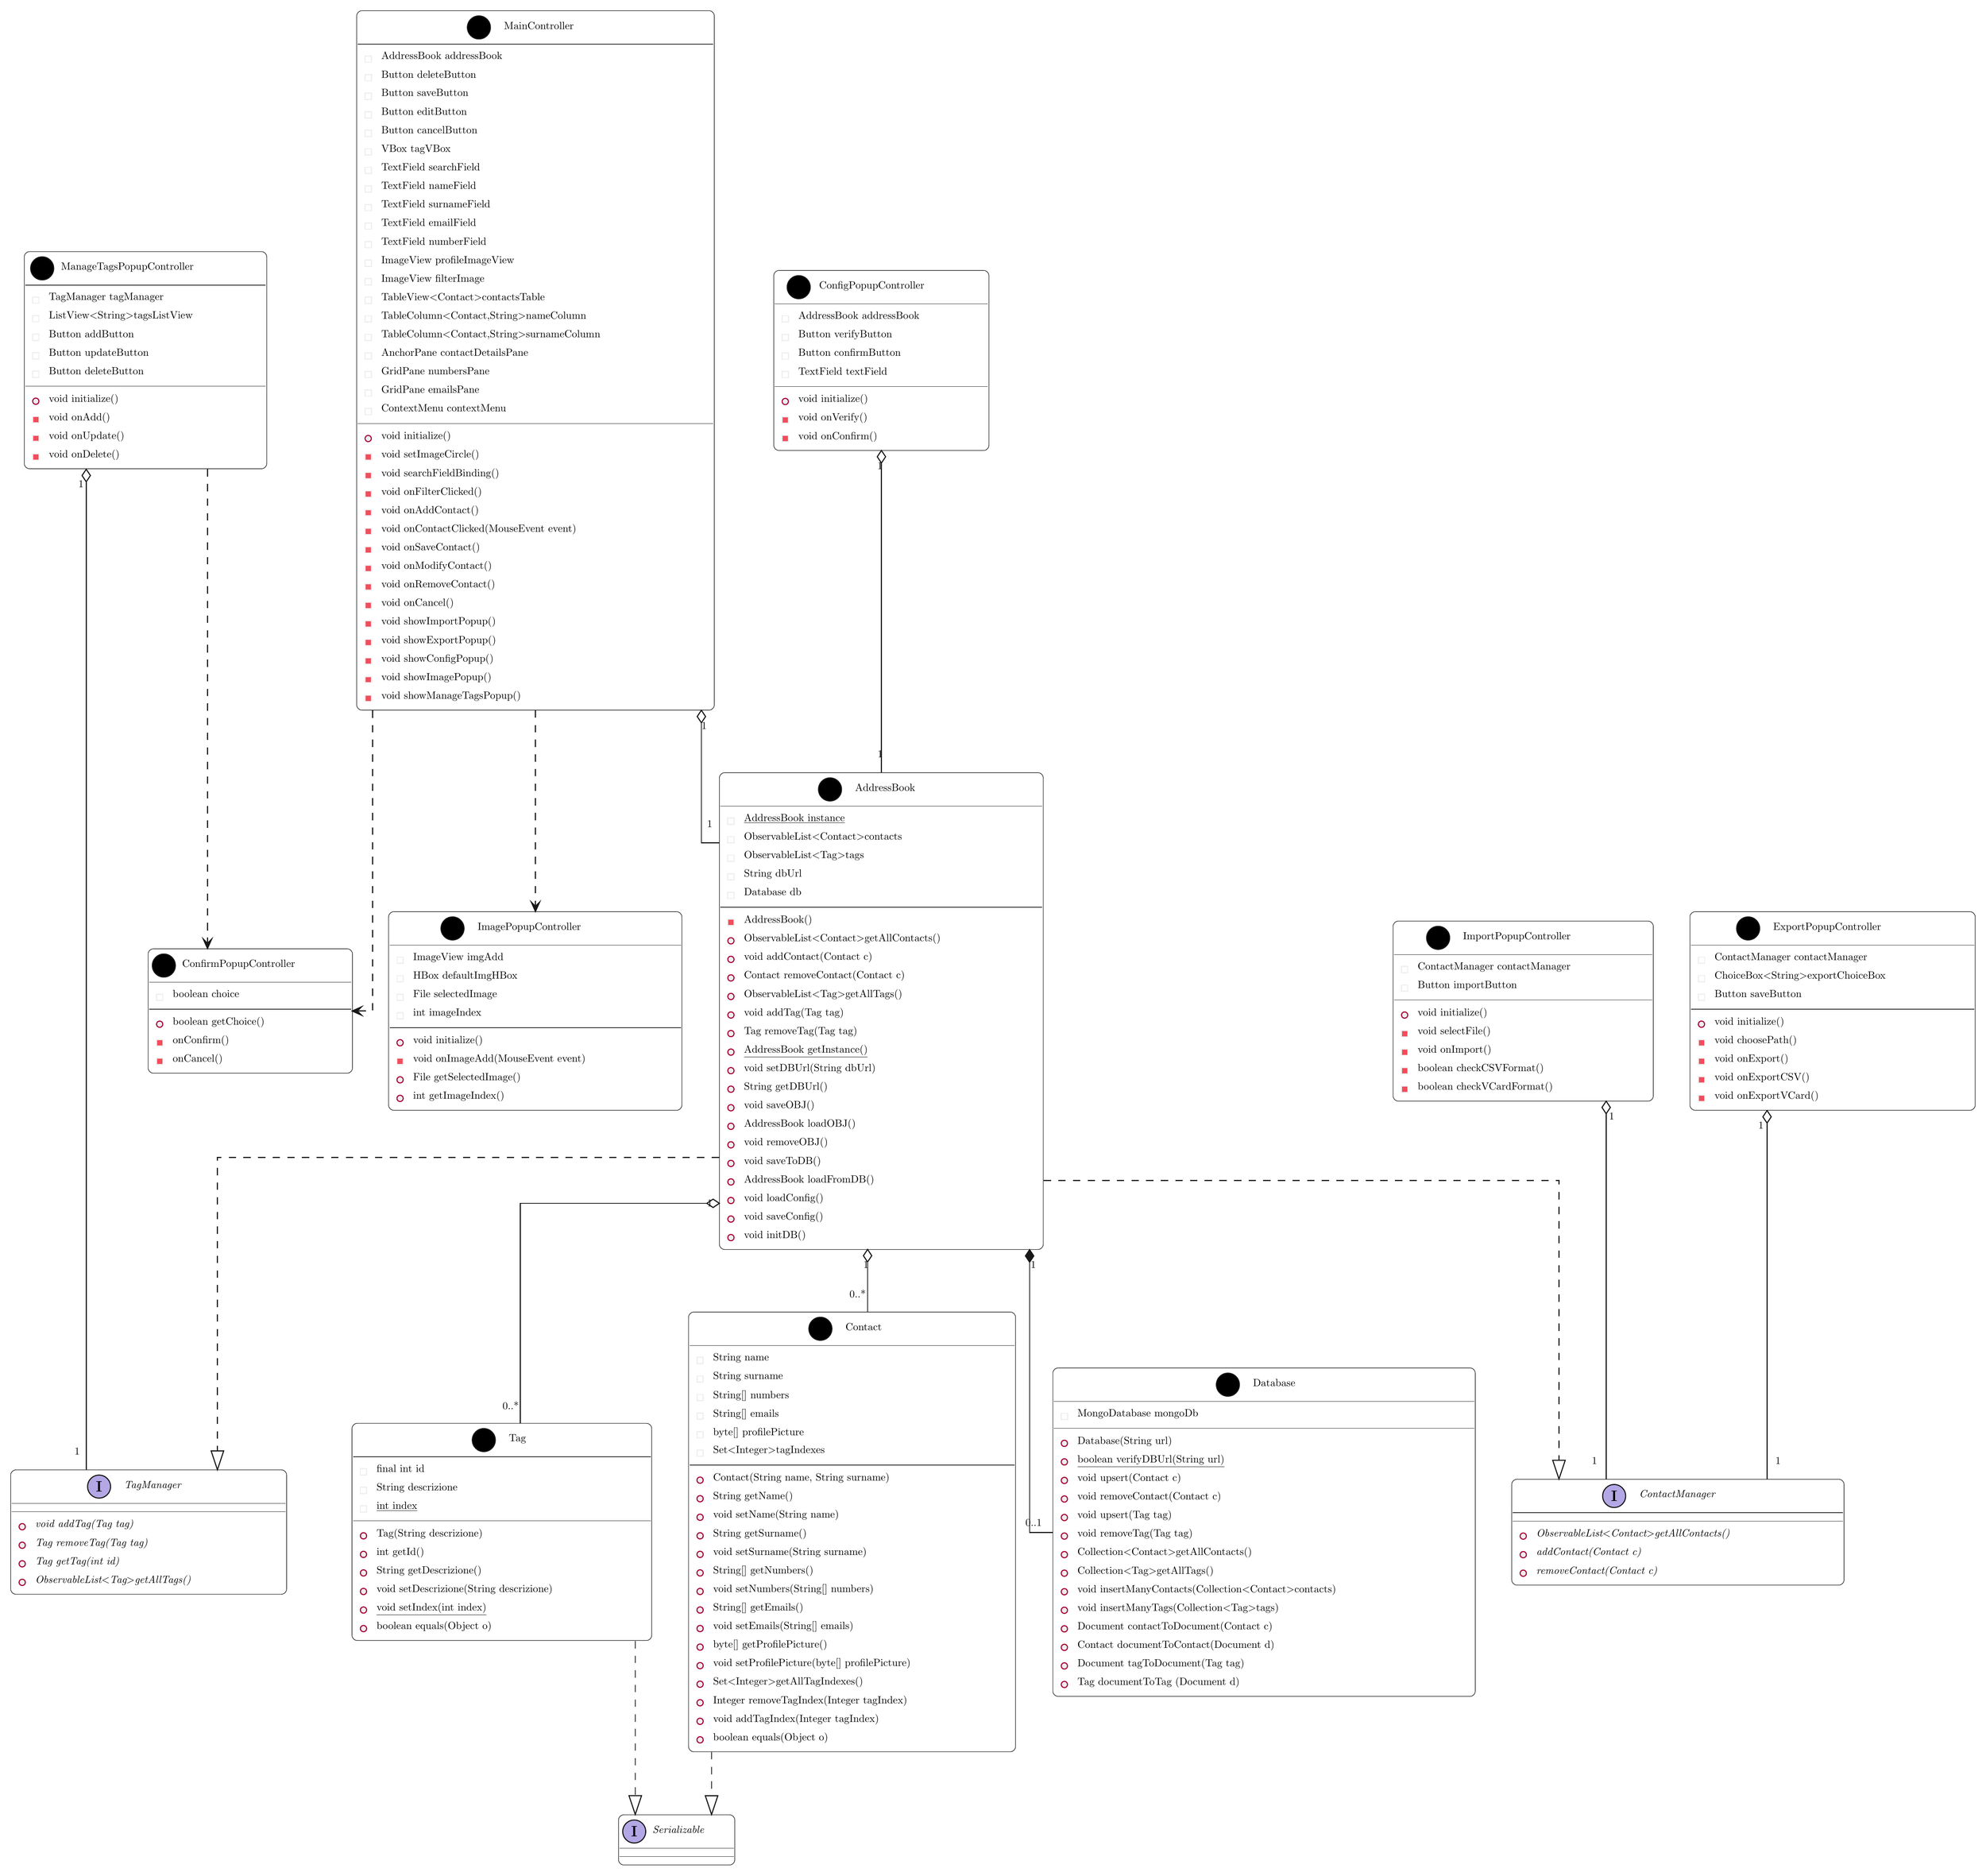
\begin{tikzpicture}[yscale=-1
,pstyle0/.style={color=plantucolor0001,fill=plantucolor0000,line width=0.5pt}
,pstyle1/.style={color=plantucolor0001,fill=plantucolor0002,line width=1.0pt}
,pstyle2/.style={color=plantucolor0001,line width=0.5pt}
,pstyle3/.style={color=plantucolor0004,line width=1.0pt}
,pstyle4/.style={color=plantucolor0006,fill=plantucolor0005,line width=1.0pt}
,pstyle5/.style={color=plantucolor0004,fill=plantucolor0007,line width=1.0pt}
,pstyle6/.style={color=plantucolor0001,fill=plantucolor0008,line width=1.0pt}
,pstyle7/.style={color=plantucolor0001,line width=1.0pt,dash pattern=on 7.0pt off 7.0pt}
,pstyle8/.style={color=plantucolor0001,line width=1.0pt}
,pstyle9/.style={color=plantucolor0001,fill=plantucolor0001,line width=1.0pt}
]
\draw[pstyle0] (333.5pt,1363.5pt) arc (180:270:5pt) -- (338.5pt,1358.5pt) -- (615.2294pt,1358.5pt) arc (270:360:5pt) -- (620.2294pt,1363.5pt) -- (620.2294pt,1561.2148pt) arc (0:90:5pt) -- (615.2294pt,1566.2148pt) -- (338.5pt,1566.2148pt) arc (90:180:5pt) -- (333.5pt,1561.2148pt) -- cycle;
\draw[pstyle1] (459.5965pt,1374.5pt) ellipse (11pt and 11pt);
\node at (459.5965pt,1374.5pt)[]{\textbf{\Large C}};
\node at (480.0965pt,1365.627pt)[below right,color=black]{Tag};
\draw[pstyle2] (334.5pt,1390.5pt) -- (619.2294pt,1390.5pt);
\draw[pstyle3] (341.5pt,1401.873pt) rectangle (347.5pt,1407.873pt);
\node at (353.5pt,1394.5pt)[below right,color=black]{final int id};
\draw[pstyle3] (341.5pt,1419.6191pt) rectangle (347.5pt,1425.6191pt);
\node at (353.5pt,1412.2461pt)[below right,color=black]{String descrizione};
\draw[pstyle3] (341.5pt,1437.3652pt) rectangle (347.5pt,1443.3652pt);
\node at (353.5pt,1429.9922pt)[below right,color=black]{\underline{int index}};
\draw[pstyle2] (334.5pt,1451.7383pt) -- (619.2294pt,1451.7383pt);
\draw[pstyle4] (344.5pt,1466.1113pt) ellipse (3pt and 3pt);
\node at (353.5pt,1455.7383pt)[below right,color=black]{Tag(String descrizione)};
\draw[pstyle4] (344.5pt,1483.8574pt) ellipse (3pt and 3pt);
\node at (353.5pt,1473.4844pt)[below right,color=black]{int getId()};
\draw[pstyle4] (344.5pt,1501.6035pt) ellipse (3pt and 3pt);
\node at (353.5pt,1491.2305pt)[below right,color=black]{String getDescrizione()};
\draw[pstyle4] (344.5pt,1519.3496pt) ellipse (3pt and 3pt);
\node at (353.5pt,1508.9766pt)[below right,color=black]{void setDescrizione(String descrizione)};
\draw[pstyle4] (344.5pt,1537.0957pt) ellipse (3pt and 3pt);
\node at (353.5pt,1526.7227pt)[below right,color=black]{\underline{void setIndex(int index)}};
\draw[pstyle4] (344.5pt,1554.8418pt) ellipse (3pt and 3pt);
\node at (353.5pt,1544.4688pt)[below right,color=black]{boolean equals(Object o)};
\draw[pstyle0] (655.5pt,1257pt) arc (180:270:5pt) -- (660.5pt,1252pt) -- (963.2837pt,1252pt) arc (270:360:5pt) -- (968.2837pt,1257pt) -- (968.2837pt,1667.668pt) arc (0:90:5pt) -- (963.2837pt,1672.668pt) -- (660.5pt,1672.668pt) arc (90:180:5pt) -- (655.5pt,1667.668pt) -- cycle;
\draw[pstyle1] (781.6055pt,1268pt) ellipse (11pt and 11pt);
\node at (781.6055pt,1268pt)[]{\textbf{\Large C}};
\node at (802.1055pt,1259.127pt)[below right,color=black]{Contact};
\draw[pstyle2] (656.5pt,1284pt) -- (967.2837pt,1284pt);
\draw[pstyle3] (663.5pt,1295.373pt) rectangle (669.5pt,1301.373pt);
\node at (675.5pt,1288pt)[below right,color=black]{String name};
\draw[pstyle3] (663.5pt,1313.1191pt) rectangle (669.5pt,1319.1191pt);
\node at (675.5pt,1305.7461pt)[below right,color=black]{String surname};
\draw[pstyle3] (663.5pt,1330.8652pt) rectangle (669.5pt,1336.8652pt);
\node at (675.5pt,1323.4922pt)[below right,color=black]{String[] numbers};
\draw[pstyle3] (663.5pt,1348.6113pt) rectangle (669.5pt,1354.6113pt);
\node at (675.5pt,1341.2383pt)[below right,color=black]{String[] emails};
\draw[pstyle3] (663.5pt,1366.3574pt) rectangle (669.5pt,1372.3574pt);
\node at (675.5pt,1358.9844pt)[below right,color=black]{byte[] profilePicture};
\draw[pstyle3] (663.5pt,1384.1035pt) rectangle (669.5pt,1390.1035pt);
\node at (675.5pt,1376.7305pt)[below right,color=black]{Set\textless Integer\textgreater  tagIndexes};
\draw[pstyle2] (656.5pt,1398.4766pt) -- (967.2837pt,1398.4766pt);
\draw[pstyle4] (666.5pt,1412.8496pt) ellipse (3pt and 3pt);
\node at (675.5pt,1402.4766pt)[below right,color=black]{Contact(String name, String surname)};
\draw[pstyle4] (666.5pt,1430.5957pt) ellipse (3pt and 3pt);
\node at (675.5pt,1420.2227pt)[below right,color=black]{String getName()};
\draw[pstyle4] (666.5pt,1448.3418pt) ellipse (3pt and 3pt);
\node at (675.5pt,1437.9688pt)[below right,color=black]{void setName(String name)};
\draw[pstyle4] (666.5pt,1466.0879pt) ellipse (3pt and 3pt);
\node at (675.5pt,1455.7148pt)[below right,color=black]{String getSurname()};
\draw[pstyle4] (666.5pt,1483.834pt) ellipse (3pt and 3pt);
\node at (675.5pt,1473.4609pt)[below right,color=black]{void setSurname(String surname)};
\draw[pstyle4] (666.5pt,1501.5801pt) ellipse (3pt and 3pt);
\node at (675.5pt,1491.207pt)[below right,color=black]{String[] getNumbers()};
\draw[pstyle4] (666.5pt,1519.3262pt) ellipse (3pt and 3pt);
\node at (675.5pt,1508.9531pt)[below right,color=black]{void setNumbers(String[] numbers)};
\draw[pstyle4] (666.5pt,1537.0723pt) ellipse (3pt and 3pt);
\node at (675.5pt,1526.6992pt)[below right,color=black]{String[] getEmails()};
\draw[pstyle4] (666.5pt,1554.8184pt) ellipse (3pt and 3pt);
\node at (675.5pt,1544.4453pt)[below right,color=black]{void setEmails(String[] emails)};
\draw[pstyle4] (666.5pt,1572.5645pt) ellipse (3pt and 3pt);
\node at (675.5pt,1562.1914pt)[below right,color=black]{byte[] getProfilePicture()};
\draw[pstyle4] (666.5pt,1590.3105pt) ellipse (3pt and 3pt);
\node at (675.5pt,1579.9375pt)[below right,color=black]{void setProfilePicture(byte[] profilePicture)};
\draw[pstyle4] (666.5pt,1608.0566pt) ellipse (3pt and 3pt);
\node at (675.5pt,1597.6836pt)[below right,color=black]{Set\textless Integer\textgreater  getAllTagIndexes()};
\draw[pstyle4] (666.5pt,1625.8027pt) ellipse (3pt and 3pt);
\node at (675.5pt,1615.4297pt)[below right,color=black]{Integer removeTagIndex(Integer tagIndex)};
\draw[pstyle4] (666.5pt,1643.5488pt) ellipse (3pt and 3pt);
\node at (675.5pt,1633.1758pt)[below right,color=black]{void addTagIndex(Integer tagIndex)};
\draw[pstyle4] (666.5pt,1661.2949pt) ellipse (3pt and 3pt);
\node at (675.5pt,1650.9219pt)[below right,color=black]{boolean equals(Object o)};
\draw[pstyle0] (685pt,741pt) arc (180:270:5pt) -- (690pt,736pt) -- (989.7833pt,736pt) arc (270:360:5pt) -- (994.7833pt,741pt) -- (994.7833pt,1187.1602pt) arc (0:90:5pt) -- (989.7833pt,1192.1602pt) -- (690pt,1192.1602pt) arc (90:180:5pt) -- (685pt,1187.1602pt) -- cycle;
\draw[pstyle1] (790.8017pt,752pt) ellipse (11pt and 11pt);
\node at (790.8017pt,752pt)[]{\textbf{\Large C}};
\node at (811.3017pt,743.127pt)[below right,color=black]{AddressBook};
\draw[pstyle2] (686pt,768pt) -- (993.7833pt,768pt);
\draw[pstyle3] (693pt,779.373pt) rectangle (699pt,785.373pt);
\node at (705pt,772pt)[below right,color=black]{\underline{AddressBook instance}};
\draw[pstyle3] (693pt,797.1191pt) rectangle (699pt,803.1191pt);
\node at (705pt,789.7461pt)[below right,color=black]{ObservableList\textless Contact\textgreater  contacts};
\draw[pstyle3] (693pt,814.8652pt) rectangle (699pt,820.8652pt);
\node at (705pt,807.4922pt)[below right,color=black]{ObservableList\textless Tag\textgreater  tags};
\draw[pstyle3] (693pt,832.6113pt) rectangle (699pt,838.6113pt);
\node at (705pt,825.2383pt)[below right,color=black]{String dbUrl};
\draw[pstyle3] (693pt,850.3574pt) rectangle (699pt,856.3574pt);
\node at (705pt,842.9844pt)[below right,color=black]{Database db};
\draw[pstyle2] (686pt,864.7305pt) -- (993.7833pt,864.7305pt);
\draw[pstyle5] (693pt,876.1035pt) rectangle (699pt,882.1035pt);
\node at (705pt,868.7305pt)[below right,color=black]{AddressBook()};
\draw[pstyle4] (696pt,896.8496pt) ellipse (3pt and 3pt);
\node at (705pt,886.4766pt)[below right,color=black]{ObservableList\textless Contact\textgreater  getAllContacts()};
\draw[pstyle4] (696pt,914.5957pt) ellipse (3pt and 3pt);
\node at (705pt,904.2227pt)[below right,color=black]{void addContact(Contact c)};
\draw[pstyle4] (696pt,932.3418pt) ellipse (3pt and 3pt);
\node at (705pt,921.9688pt)[below right,color=black]{Contact removeContact(Contact c)};
\draw[pstyle4] (696pt,950.0879pt) ellipse (3pt and 3pt);
\node at (705pt,939.7148pt)[below right,color=black]{ObservableList\textless Tag\textgreater  getAllTags()};
\draw[pstyle4] (696pt,967.834pt) ellipse (3pt and 3pt);
\node at (705pt,957.4609pt)[below right,color=black]{void addTag(Tag tag)};
\draw[pstyle4] (696pt,985.5801pt) ellipse (3pt and 3pt);
\node at (705pt,975.207pt)[below right,color=black]{Tag removeTag(Tag tag)};
\draw[pstyle4] (696pt,1003.3262pt) ellipse (3pt and 3pt);
\node at (705pt,992.9531pt)[below right,color=black]{\underline{AddressBook getInstance()}};
\draw[pstyle4] (696pt,1021.0723pt) ellipse (3pt and 3pt);
\node at (705pt,1010.6992pt)[below right,color=black]{void setDBUrl(String dbUrl)};
\draw[pstyle4] (696pt,1038.8184pt) ellipse (3pt and 3pt);
\node at (705pt,1028.4453pt)[below right,color=black]{String getDBUrl()};
\draw[pstyle4] (696pt,1056.5645pt) ellipse (3pt and 3pt);
\node at (705pt,1046.1914pt)[below right,color=black]{void saveOBJ()};
\draw[pstyle4] (696pt,1074.3105pt) ellipse (3pt and 3pt);
\node at (705pt,1063.9375pt)[below right,color=black]{AddressBook loadOBJ()};
\draw[pstyle4] (696pt,1092.0566pt) ellipse (3pt and 3pt);
\node at (705pt,1081.6836pt)[below right,color=black]{void removeOBJ()};
\draw[pstyle4] (696pt,1109.8027pt) ellipse (3pt and 3pt);
\node at (705pt,1099.4297pt)[below right,color=black]{void saveToDB()};
\draw[pstyle4] (696pt,1127.5488pt) ellipse (3pt and 3pt);
\node at (705pt,1117.1758pt)[below right,color=black]{AddressBook loadFromDB()};
\draw[pstyle4] (696pt,1145.2949pt) ellipse (3pt and 3pt);
\node at (705pt,1134.9219pt)[below right,color=black]{void loadConfig()};
\draw[pstyle4] (696pt,1163.041pt) ellipse (3pt and 3pt);
\node at (705pt,1152.668pt)[below right,color=black]{void saveConfig()};
\draw[pstyle4] (696pt,1180.7871pt) ellipse (3pt and 3pt);
\node at (705pt,1170.4141pt)[below right,color=black]{void initDB()};
\draw[pstyle0] (338pt,12pt) arc (180:270:5pt) -- (343pt,7pt) -- (675.1086pt,7pt) arc (270:360:5pt) -- (680.1086pt,12pt) -- (680.1086pt,671.1133pt) arc (0:90:5pt) -- (675.1086pt,676.1133pt) -- (343pt,676.1133pt) arc (90:180:5pt) -- (338pt,671.1133pt) -- cycle;
\draw[pstyle1] (454.9043pt,23pt) ellipse (11pt and 11pt);
\node at (454.9043pt,23pt)[]{\textbf{\Large C}};
\node at (475.4043pt,14.127pt)[below right,color=black]{MainController};
\draw[pstyle2] (339pt,39pt) -- (679.1086pt,39pt);
\draw[pstyle3] (346pt,50.373pt) rectangle (352pt,56.373pt);
\node at (358pt,43pt)[below right,color=black]{AddressBook addressBook};
\draw[pstyle3] (346pt,68.1191pt) rectangle (352pt,74.1191pt);
\node at (358pt,60.7461pt)[below right,color=black]{Button deleteButton};
\draw[pstyle3] (346pt,85.8652pt) rectangle (352pt,91.8652pt);
\node at (358pt,78.4922pt)[below right,color=black]{Button saveButton};
\draw[pstyle3] (346pt,103.6113pt) rectangle (352pt,109.6113pt);
\node at (358pt,96.2383pt)[below right,color=black]{Button editButton};
\draw[pstyle3] (346pt,121.3574pt) rectangle (352pt,127.3574pt);
\node at (358pt,113.9844pt)[below right,color=black]{Button cancelButton};
\draw[pstyle3] (346pt,139.1035pt) rectangle (352pt,145.1035pt);
\node at (358pt,131.7305pt)[below right,color=black]{VBox tagVBox};
\draw[pstyle3] (346pt,156.8496pt) rectangle (352pt,162.8496pt);
\node at (358pt,149.4766pt)[below right,color=black]{TextField searchField};
\draw[pstyle3] (346pt,174.5957pt) rectangle (352pt,180.5957pt);
\node at (358pt,167.2227pt)[below right,color=black]{TextField nameField};
\draw[pstyle3] (346pt,192.3418pt) rectangle (352pt,198.3418pt);
\node at (358pt,184.9688pt)[below right,color=black]{TextField surnameField};
\draw[pstyle3] (346pt,210.0879pt) rectangle (352pt,216.0879pt);
\node at (358pt,202.7148pt)[below right,color=black]{TextField emailField};
\draw[pstyle3] (346pt,227.834pt) rectangle (352pt,233.834pt);
\node at (358pt,220.4609pt)[below right,color=black]{TextField numberField};
\draw[pstyle3] (346pt,245.5801pt) rectangle (352pt,251.5801pt);
\node at (358pt,238.207pt)[below right,color=black]{ImageView profileImageView};
\draw[pstyle3] (346pt,263.3262pt) rectangle (352pt,269.3262pt);
\node at (358pt,255.9531pt)[below right,color=black]{ImageView filterImage};
\draw[pstyle3] (346pt,281.0723pt) rectangle (352pt,287.0723pt);
\node at (358pt,273.6992pt)[below right,color=black]{TableView\textless Contact\textgreater  contactsTable};
\draw[pstyle3] (346pt,298.8184pt) rectangle (352pt,304.8184pt);
\node at (358pt,291.4453pt)[below right,color=black]{TableColumn\textless Contact,String\textgreater  nameColumn};
\draw[pstyle3] (346pt,316.5645pt) rectangle (352pt,322.5645pt);
\node at (358pt,309.1914pt)[below right,color=black]{TableColumn\textless Contact,String\textgreater  surnameColumn};
\draw[pstyle3] (346pt,334.3105pt) rectangle (352pt,340.3105pt);
\node at (358pt,326.9375pt)[below right,color=black]{AnchorPane contactDetailsPane};
\draw[pstyle3] (346pt,352.0566pt) rectangle (352pt,358.0566pt);
\node at (358pt,344.6836pt)[below right,color=black]{GridPane numbersPane};
\draw[pstyle3] (346pt,369.8027pt) rectangle (352pt,375.8027pt);
\node at (358pt,362.4297pt)[below right,color=black]{GridPane emailsPane};
\draw[pstyle3] (346pt,387.5488pt) rectangle (352pt,393.5488pt);
\node at (358pt,380.1758pt)[below right,color=black]{ContextMenu contextMenu};
\draw[pstyle2] (339pt,401.9219pt) -- (679.1086pt,401.9219pt);
\draw[pstyle4] (349pt,416.2949pt) ellipse (3pt and 3pt);
\node at (358pt,405.9219pt)[below right,color=black]{void initialize()};
\draw[pstyle5] (346pt,431.041pt) rectangle (352pt,437.041pt);
\node at (358pt,423.668pt)[below right,color=black]{void setImageCircle()};
\draw[pstyle5] (346pt,448.7871pt) rectangle (352pt,454.7871pt);
\node at (358pt,441.4141pt)[below right,color=black]{void searchFieldBinding()};
\draw[pstyle5] (346pt,466.5332pt) rectangle (352pt,472.5332pt);
\node at (358pt,459.1602pt)[below right,color=black]{void onFilterClicked()};
\draw[pstyle5] (346pt,484.2793pt) rectangle (352pt,490.2793pt);
\node at (358pt,476.9063pt)[below right,color=black]{void onAddContact()};
\draw[pstyle5] (346pt,502.0254pt) rectangle (352pt,508.0254pt);
\node at (358pt,494.6523pt)[below right,color=black]{void onContactClicked(MouseEvent event)};
\draw[pstyle5] (346pt,519.7715pt) rectangle (352pt,525.7715pt);
\node at (358pt,512.3984pt)[below right,color=black]{void onSaveContact()};
\draw[pstyle5] (346pt,537.5176pt) rectangle (352pt,543.5176pt);
\node at (358pt,530.1445pt)[below right,color=black]{void onModifyContact()};
\draw[pstyle5] (346pt,555.2637pt) rectangle (352pt,561.2637pt);
\node at (358pt,547.8906pt)[below right,color=black]{void onRemoveContact()};
\draw[pstyle5] (346pt,573.0098pt) rectangle (352pt,579.0098pt);
\node at (358pt,565.6367pt)[below right,color=black]{void onCancel()};
\draw[pstyle5] (346pt,590.7559pt) rectangle (352pt,596.7559pt);
\node at (358pt,583.3828pt)[below right,color=black]{void showImportPopup()};
\draw[pstyle5] (346pt,608.502pt) rectangle (352pt,614.502pt);
\node at (358pt,601.1289pt)[below right,color=black]{void showExportPopup()};
\draw[pstyle5] (346pt,626.248pt) rectangle (352pt,632.248pt);
\node at (358pt,618.875pt)[below right,color=black]{void showConfigPopup()};
\draw[pstyle5] (346pt,643.9941pt) rectangle (352pt,649.9941pt);
\node at (358pt,636.6211pt)[below right,color=black]{void showImagePopup()};
\draw[pstyle5] (346pt,661.7402pt) rectangle (352pt,667.7402pt);
\node at (358pt,654.3672pt)[below right,color=black]{void showManageTagsPopup()};
\draw[pstyle0] (1329.5pt,883pt) arc (180:270:5pt) -- (1334.5pt,878pt) -- (1573.4191pt,878pt) arc (270:360:5pt) -- (1578.4191pt,883pt) -- (1578.4191pt,1045.2227pt) arc (0:90:5pt) -- (1573.4191pt,1050.2227pt) -- (1334.5pt,1050.2227pt) arc (90:180:5pt) -- (1329.5pt,1045.2227pt) -- cycle;
\draw[pstyle1] (1372.5828pt,894pt) ellipse (11pt and 11pt);
\node at (1372.5828pt,894pt)[]{\textbf{\Large C}};
\node at (1392.8234pt,885.127pt)[below right,color=black]{ImportPopupController};
\draw[pstyle2] (1330.5pt,910pt) -- (1577.4191pt,910pt);
\draw[pstyle3] (1337.5pt,921.373pt) rectangle (1343.5pt,927.373pt);
\node at (1349.5pt,914pt)[below right,color=black]{ContactManager contactManager};
\draw[pstyle3] (1337.5pt,939.1191pt) rectangle (1343.5pt,945.1191pt);
\node at (1349.5pt,931.7461pt)[below right,color=black]{Button importButton};
\draw[pstyle2] (1330.5pt,953.4922pt) -- (1577.4191pt,953.4922pt);
\draw[pstyle4] (1340.5pt,967.8652pt) ellipse (3pt and 3pt);
\node at (1349.5pt,957.4922pt)[below right,color=black]{void initialize()};
\draw[pstyle5] (1337.5pt,982.6113pt) rectangle (1343.5pt,988.6113pt);
\node at (1349.5pt,975.2383pt)[below right,color=black]{void selectFile()};
\draw[pstyle5] (1337.5pt,1000.3574pt) rectangle (1343.5pt,1006.3574pt);
\node at (1349.5pt,992.9844pt)[below right,color=black]{void onImport()};
\draw[pstyle5] (1337.5pt,1018.1035pt) rectangle (1343.5pt,1024.1035pt);
\node at (1349.5pt,1010.7305pt)[below right,color=black]{boolean checkCSVFormat()};
\draw[pstyle5] (1337.5pt,1035.8496pt) rectangle (1343.5pt,1041.8496pt);
\node at (1349.5pt,1028.4766pt)[below right,color=black]{boolean checkVCardFormat()};
\draw[pstyle0] (1613.5pt,874pt) arc (180:270:5pt) -- (1618.5pt,869pt) -- (1881.3528pt,869pt) arc (270:360:5pt) -- (1886.3528pt,874pt) -- (1886.3528pt,1053.9688pt) arc (0:90:5pt) -- (1881.3528pt,1058.9688pt) -- (1618.5pt,1058.9688pt) arc (90:180:5pt) -- (1613.5pt,1053.9688pt) -- cycle;
\draw[pstyle1] (1669.1533pt,885pt) ellipse (11pt and 11pt);
\node at (1669.1533pt,885pt)[]{\textbf{\Large C}};
\node at (1689.6533pt,876.127pt)[below right,color=black]{ExportPopupController};
\draw[pstyle2] (1614.5pt,901pt) -- (1885.3528pt,901pt);
\draw[pstyle3] (1621.5pt,912.373pt) rectangle (1627.5pt,918.373pt);
\node at (1633.5pt,905pt)[below right,color=black]{ContactManager contactManager};
\draw[pstyle3] (1621.5pt,930.1191pt) rectangle (1627.5pt,936.1191pt);
\node at (1633.5pt,922.7461pt)[below right,color=black]{ChoiceBox\textless String\textgreater  exportChoiceBox};
\draw[pstyle3] (1621.5pt,947.8652pt) rectangle (1627.5pt,953.8652pt);
\node at (1633.5pt,940.4922pt)[below right,color=black]{Button saveButton};
\draw[pstyle2] (1614.5pt,962.2383pt) -- (1885.3528pt,962.2383pt);
\draw[pstyle4] (1624.5pt,976.6113pt) ellipse (3pt and 3pt);
\node at (1633.5pt,966.2383pt)[below right,color=black]{void initialize()};
\draw[pstyle5] (1621.5pt,991.3574pt) rectangle (1627.5pt,997.3574pt);
\node at (1633.5pt,983.9844pt)[below right,color=black]{void choosePath()};
\draw[pstyle5] (1621.5pt,1009.1035pt) rectangle (1627.5pt,1015.1035pt);
\node at (1633.5pt,1001.7305pt)[below right,color=black]{void onExport()};
\draw[pstyle5] (1621.5pt,1026.8496pt) rectangle (1627.5pt,1032.8496pt);
\node at (1633.5pt,1019.4766pt)[below right,color=black]{void onExportCSV()};
\draw[pstyle5] (1621.5pt,1044.5957pt) rectangle (1627.5pt,1050.5957pt);
\node at (1633.5pt,1037.2227pt)[below right,color=black]{void onExportVCard()};
\draw[pstyle0] (20pt,242.5pt) arc (180:270:5pt) -- (25pt,237.5pt) -- (246.9367pt,237.5pt) arc (270:360:5pt) -- (251.9367pt,242.5pt) -- (251.9367pt,440.2148pt) arc (0:90:5pt) -- (246.9367pt,445.2148pt) -- (25pt,445.2148pt) arc (90:180:5pt) -- (20pt,440.2148pt) -- cycle;
\draw[pstyle1] (37.1249pt,253.5pt) ellipse (11pt and 11pt);
\node at (37.1249pt,253.5pt)[]{\textbf{\Large C}};
\node at (51.5971pt,244.627pt)[below right,color=black]{ManageTagsPopupController};
\draw[pstyle2] (21pt,269.5pt) -- (250.9367pt,269.5pt);
\draw[pstyle3] (28pt,280.873pt) rectangle (34pt,286.873pt);
\node at (40pt,273.5pt)[below right,color=black]{TagManager tagManager};
\draw[pstyle3] (28pt,298.6191pt) rectangle (34pt,304.6191pt);
\node at (40pt,291.2461pt)[below right,color=black]{ListView\textless String\textgreater  tagsListView};
\draw[pstyle3] (28pt,316.3652pt) rectangle (34pt,322.3652pt);
\node at (40pt,308.9922pt)[below right,color=black]{Button addButton};
\draw[pstyle3] (28pt,334.1113pt) rectangle (34pt,340.1113pt);
\node at (40pt,326.7383pt)[below right,color=black]{Button updateButton};
\draw[pstyle3] (28pt,351.8574pt) rectangle (34pt,357.8574pt);
\node at (40pt,344.4844pt)[below right,color=black]{Button deleteButton};
\draw[pstyle2] (21pt,366.2305pt) -- (250.9367pt,366.2305pt);
\draw[pstyle4] (31pt,380.6035pt) ellipse (3pt and 3pt);
\node at (40pt,370.2305pt)[below right,color=black]{void initialize()};
\draw[pstyle5] (28pt,395.3496pt) rectangle (34pt,401.3496pt);
\node at (40pt,387.9766pt)[below right,color=black]{void onAdd()};
\draw[pstyle5] (28pt,413.0957pt) rectangle (34pt,419.0957pt);
\node at (40pt,405.7227pt)[below right,color=black]{void onUpdate()};
\draw[pstyle5] (28pt,430.8418pt) rectangle (34pt,436.8418pt);
\node at (40pt,423.4688pt)[below right,color=black]{void onDelete()};
\draw[pstyle0] (368.5pt,874pt) arc (180:270:5pt) -- (373.5pt,869pt) -- (644.0757pt,869pt) arc (270:360:5pt) -- (649.0757pt,874pt) -- (649.0757pt,1053.9688pt) arc (0:90:5pt) -- (644.0757pt,1058.9688pt) -- (373.5pt,1058.9688pt) arc (90:180:5pt) -- (368.5pt,1053.9688pt) -- cycle;
\draw[pstyle1] (429.6607pt,885pt) ellipse (11pt and 11pt);
\node at (429.6607pt,885pt)[]{\textbf{\Large C}};
\node at (450.1607pt,876.127pt)[below right,color=black]{ImagePopupController};
\draw[pstyle2] (369.5pt,901pt) -- (648.0757pt,901pt);
\draw[pstyle3] (376.5pt,912.373pt) rectangle (382.5pt,918.373pt);
\node at (388.5pt,905pt)[below right,color=black]{ImageView imgAdd};
\draw[pstyle3] (376.5pt,930.1191pt) rectangle (382.5pt,936.1191pt);
\node at (388.5pt,922.7461pt)[below right,color=black]{HBox defaultImgHBox};
\draw[pstyle3] (376.5pt,947.8652pt) rectangle (382.5pt,953.8652pt);
\node at (388.5pt,940.4922pt)[below right,color=black]{File selectedImage};
\draw[pstyle3] (376.5pt,965.6113pt) rectangle (382.5pt,971.6113pt);
\node at (388.5pt,958.2383pt)[below right,color=black]{int imageIndex};
\draw[pstyle2] (369.5pt,979.9844pt) -- (648.0757pt,979.9844pt);
\draw[pstyle4] (379.5pt,994.3574pt) ellipse (3pt and 3pt);
\node at (388.5pt,983.9844pt)[below right,color=black]{void initialize()};
\draw[pstyle5] (376.5pt,1009.1035pt) rectangle (382.5pt,1015.1035pt);
\node at (388.5pt,1001.7305pt)[below right,color=black]{void onImageAdd(MouseEvent event)};
\draw[pstyle4] (379.5pt,1029.8496pt) ellipse (3pt and 3pt);
\node at (388.5pt,1019.4766pt)[below right,color=black]{File getSelectedImage()};
\draw[pstyle4] (379.5pt,1047.5957pt) ellipse (3pt and 3pt);
\node at (388.5pt,1037.2227pt)[below right,color=black]{int getImageIndex()};
\draw[pstyle0] (138.5pt,909.5pt) arc (180:270:5pt) -- (143.5pt,904.5pt) -- (328.9331pt,904.5pt) arc (270:360:5pt) -- (333.9331pt,909.5pt) -- (333.9331pt,1018.4844pt) arc (0:90:5pt) -- (328.9331pt,1023.4844pt) -- (143.5pt,1023.4844pt) arc (90:180:5pt) -- (138.5pt,1018.4844pt) -- cycle;
\draw[pstyle1] (153.5pt,920.5pt) ellipse (11pt and 11pt);
\node at (153.5pt,920.5pt)[]{\textbf{\Large C}};
\node at (167.5pt,911.627pt)[below right,color=black]{ConfirmPopupController};
\draw[pstyle2] (139.5pt,936.5pt) -- (332.9331pt,936.5pt);
\draw[pstyle3] (146.5pt,947.873pt) rectangle (152.5pt,953.873pt);
\node at (158.5pt,940.5pt)[below right,color=black]{boolean choice};
\draw[pstyle2] (139.5pt,962.2461pt) -- (332.9331pt,962.2461pt);
\draw[pstyle4] (149.5pt,976.6191pt) ellipse (3pt and 3pt);
\node at (158.5pt,966.2461pt)[below right,color=black]{boolean getChoice()};
\draw[pstyle5] (146.5pt,991.3652pt) rectangle (152.5pt,997.3652pt);
\node at (158.5pt,983.9922pt)[below right,color=black]{onConfirm()};
\draw[pstyle5] (146.5pt,1009.1113pt) rectangle (152.5pt,1015.1113pt);
\node at (158.5pt,1001.7383pt)[below right,color=black]{onCancel()};
\draw[pstyle0] (737pt,260.5pt) arc (180:270:5pt) -- (742pt,255.5pt) -- (937.8225pt,255.5pt) arc (270:360:5pt) -- (942.8225pt,260.5pt) -- (942.8225pt,422.7227pt) arc (0:90:5pt) -- (937.8225pt,427.7227pt) -- (742pt,427.7227pt) arc (90:180:5pt) -- (737pt,422.7227pt) -- cycle;
\draw[pstyle1] (760.8509pt,271.5pt) ellipse (11pt and 11pt);
\node at (760.8509pt,271.5pt)[]{\textbf{\Large C}};
\node at (776.8178pt,262.627pt)[below right,color=black]{ConfigPopupController};
\draw[pstyle2] (738pt,287.5pt) -- (941.8225pt,287.5pt);
\draw[pstyle3] (745pt,298.873pt) rectangle (751pt,304.873pt);
\node at (757pt,291.5pt)[below right,color=black]{AddressBook addressBook};
\draw[pstyle3] (745pt,316.6191pt) rectangle (751pt,322.6191pt);
\node at (757pt,309.2461pt)[below right,color=black]{Button verifyButton};
\draw[pstyle3] (745pt,334.3652pt) rectangle (751pt,340.3652pt);
\node at (757pt,326.9922pt)[below right,color=black]{Button confirmButton};
\draw[pstyle3] (745pt,352.1113pt) rectangle (751pt,358.1113pt);
\node at (757pt,344.7383pt)[below right,color=black]{TextField textField};
\draw[pstyle2] (738pt,366.4844pt) -- (941.8225pt,366.4844pt);
\draw[pstyle4] (748pt,380.8574pt) ellipse (3pt and 3pt);
\node at (757pt,370.4844pt)[below right,color=black]{void initialize()};
\draw[pstyle5] (745pt,395.6035pt) rectangle (751pt,401.6035pt);
\node at (757pt,388.2305pt)[below right,color=black]{void onVerify()};
\draw[pstyle5] (745pt,413.3496pt) rectangle (751pt,419.3496pt);
\node at (757pt,405.9766pt)[below right,color=black]{void onConfirm()};
\draw[pstyle0] (1004pt,1310.5pt) arc (180:270:5pt) -- (1009pt,1305.5pt) -- (1403.0978pt,1305.5pt) arc (270:360:5pt) -- (1408.0978pt,1310.5pt) -- (1408.0978pt,1614.6914pt) arc (0:90:5pt) -- (1403.0978pt,1619.6914pt) -- (1009pt,1619.6914pt) arc (90:180:5pt) -- (1004pt,1614.6914pt) -- cycle;
\draw[pstyle1] (1171.4342pt,1321.5pt) ellipse (11pt and 11pt);
\node at (1171.4342pt,1321.5pt)[]{\textbf{\Large C}};
\node at (1191.9342pt,1312.627pt)[below right,color=black]{Database};
\draw[pstyle2] (1005pt,1337.5pt) -- (1407.0978pt,1337.5pt);
\draw[pstyle3] (1012pt,1348.873pt) rectangle (1018pt,1354.873pt);
\node at (1024pt,1341.5pt)[below right,color=black]{MongoDatabase mongoDb};
\draw[pstyle2] (1005pt,1363.2461pt) -- (1407.0978pt,1363.2461pt);
\draw[pstyle4] (1015pt,1377.6191pt) ellipse (3pt and 3pt);
\node at (1024pt,1367.2461pt)[below right,color=black]{Database(String url)};
\draw[pstyle4] (1015pt,1395.3652pt) ellipse (3pt and 3pt);
\node at (1024pt,1384.9922pt)[below right,color=black]{\underline{boolean verifyDBUrl(String url)}};
\draw[pstyle4] (1015pt,1413.1113pt) ellipse (3pt and 3pt);
\node at (1024pt,1402.7383pt)[below right,color=black]{void upsert(Contact c)};
\draw[pstyle4] (1015pt,1430.8574pt) ellipse (3pt and 3pt);
\node at (1024pt,1420.4844pt)[below right,color=black]{void removeContact(Contact c)};
\draw[pstyle4] (1015pt,1448.6035pt) ellipse (3pt and 3pt);
\node at (1024pt,1438.2305pt)[below right,color=black]{void upsert(Tag tag)};
\draw[pstyle4] (1015pt,1466.3496pt) ellipse (3pt and 3pt);
\node at (1024pt,1455.9766pt)[below right,color=black]{void removeTag(Tag tag)};
\draw[pstyle4] (1015pt,1484.0957pt) ellipse (3pt and 3pt);
\node at (1024pt,1473.7227pt)[below right,color=black]{Collection\textless Contact\textgreater  getAllContacts()};
\draw[pstyle4] (1015pt,1501.8418pt) ellipse (3pt and 3pt);
\node at (1024pt,1491.4688pt)[below right,color=black]{Collection\textless Tag\textgreater  getAllTags()};
\draw[pstyle4] (1015pt,1519.5879pt) ellipse (3pt and 3pt);
\node at (1024pt,1509.2148pt)[below right,color=black]{void insertManyContacts(Collection\textless Contact\textgreater  contacts)};
\draw[pstyle4] (1015pt,1537.334pt) ellipse (3pt and 3pt);
\node at (1024pt,1526.9609pt)[below right,color=black]{void insertManyTags(Collection\textless Tag\textgreater  tags)};
\draw[pstyle4] (1015pt,1555.0801pt) ellipse (3pt and 3pt);
\node at (1024pt,1544.707pt)[below right,color=black]{Document contactToDocument(Contact c)};
\draw[pstyle4] (1015pt,1572.8262pt) ellipse (3pt and 3pt);
\node at (1024pt,1562.4531pt)[below right,color=black]{Contact documentToContact(Document d)};
\draw[pstyle4] (1015pt,1590.5723pt) ellipse (3pt and 3pt);
\node at (1024pt,1580.1992pt)[below right,color=black]{Document tagToDocument(Tag tag)};
\draw[pstyle4] (1015pt,1608.3184pt) ellipse (3pt and 3pt);
\node at (1024pt,1597.9453pt)[below right,color=black]{Tag documentToTag (Document d)};
\draw[pstyle0] (588.5pt,1738pt) arc (180:270:5pt) -- (593.5pt,1733pt) -- (694.7pt,1733pt) arc (270:360:5pt) -- (699.7pt,1738pt) -- (699.7pt,1776pt) arc (0:90:5pt) -- (694.7pt,1781pt) -- (593.5pt,1781pt) arc (90:180:5pt) -- (588.5pt,1776pt) -- cycle;
\draw[pstyle6] (603.5pt,1749pt) ellipse (11pt and 11pt);
\node at (603.5pt,1749pt)[]{\textbf{\Large I}};
\node at (617.5pt,1740.127pt)[below right,color=black]{\textit{Serializable}};
\draw[pstyle2] (589.5pt,1765pt) -- (698.7pt,1765pt);
\draw[pstyle2] (589.5pt,1773pt) -- (698.7pt,1773pt);
\draw[pstyle0] (7pt,1408pt) arc (180:270:5pt) -- (12pt,1403pt) -- (265.9446pt,1403pt) arc (270:360:5pt) -- (270.9446pt,1408pt) -- (270.9446pt,1516.9844pt) arc (0:90:5pt) -- (265.9446pt,1521.9844pt) -- (12pt,1521.9844pt) arc (90:180:5pt) -- (7pt,1516.9844pt) -- cycle;
\draw[pstyle6] (91.525pt,1419pt) ellipse (11pt and 11pt);
\node at (91.525pt,1419pt)[]{\textbf{\Large I}};
\node at (112.025pt,1410.127pt)[below right,color=black]{\textit{TagManager}};
\draw[pstyle2] (8pt,1435pt) -- (269.9446pt,1435pt);
\draw[pstyle2] (8pt,1443pt) -- (269.9446pt,1443pt);
\draw[pstyle4] (18pt,1457.373pt) ellipse (3pt and 3pt);
\node at (27pt,1447pt)[below right,color=black]{\textit{void addTag(Tag tag)}};
\draw[pstyle4] (18pt,1475.1191pt) ellipse (3pt and 3pt);
\node at (27pt,1464.7461pt)[below right,color=black]{\textit{Tag removeTag(Tag tag)}};
\draw[pstyle4] (18pt,1492.8652pt) ellipse (3pt and 3pt);
\node at (27pt,1482.4922pt)[below right,color=black]{\textit{Tag getTag(int id)}};
\draw[pstyle4] (18pt,1510.6113pt) ellipse (3pt and 3pt);
\node at (27pt,1500.2383pt)[below right,color=black]{\textit{ObservableList\textless Tag\textgreater  getAllTags()}};
\draw[pstyle0] (1443pt,1417pt) arc (180:270:5pt) -- (1448pt,1412pt) -- (1755.8992pt,1412pt) arc (270:360:5pt) -- (1760.8992pt,1417pt) -- (1760.8992pt,1508.2383pt) arc (0:90:5pt) -- (1755.8992pt,1513.2383pt) -- (1448pt,1513.2383pt) arc (90:180:5pt) -- (1443pt,1508.2383pt) -- cycle;
\draw[pstyle6] (1540.9733pt,1428pt) ellipse (11pt and 11pt);
\node at (1540.9733pt,1428pt)[]{\textbf{\Large I}};
\node at (1561.4733pt,1419.127pt)[below right,color=black]{\textit{ContactManager}};
\draw[pstyle2] (1444pt,1444pt) -- (1759.8992pt,1444pt);
\draw[pstyle2] (1444pt,1452pt) -- (1759.8992pt,1452pt);
\draw[pstyle4] (1454pt,1466.373pt) ellipse (3pt and 3pt);
\node at (1463pt,1456pt)[below right,color=black]{\textit{ObservableList\textless Contact\textgreater  getAllContacts()}};
\draw[pstyle4] (1454pt,1484.1191pt) ellipse (3pt and 3pt);
\node at (1463pt,1473.7461pt)[below right,color=black]{\textit{addContact(Contact c)}};
\draw[pstyle4] (1454pt,1501.8652pt) ellipse (3pt and 3pt);
\node at (1463pt,1491.4922pt)[below right,color=black]{\textit{removeContact(Contact c)}};
\draw[pstyle7] (677.5pt,1673pt) ..controls (677.5pt,1696.7pt) and (677.5pt,1699.7pt) .. (677.5pt,1714.77pt);
\draw[pstyle8] (677.5pt,1732.77pt) -- (683.5pt,1714.77pt) -- (671.5pt,1714.77pt) -- (677.5pt,1732.77pt) -- cycle;
\draw[pstyle7] (604.5pt,1566.74pt) ..controls (604.5pt,1626.48pt) and (604.5pt,1678.56pt) .. (604.5pt,1714.7pt);
\draw[pstyle8] (604.5pt,1732.7pt) -- (610.5pt,1714.7pt) -- (598.5pt,1714.7pt) -- (604.5pt,1732.7pt) -- cycle;
\draw[pstyle8] (826.75pt,1204.1pt) ..controls (826.75pt,1223.96pt) and (826.75pt,1232.01pt) .. (826.75pt,1251.73pt);
\draw[pstyle8] (826.75pt,1192.1pt) -- (822.75pt,1198.1pt) -- (826.75pt,1204.1pt) -- (830.75pt,1198.1pt) -- (826.75pt,1192.1pt) -- cycle;
\node at (819.2072pt,1199.8523pt)[below right,color=black]{1};
\node at (805.9389pt,1227.2001pt)[below right,color=black]{0..*};
\draw[pstyle8] (981.75pt,1204.32pt) ..controls (981.75pt,1335.72pt) and (981.75pt,1463pt) .. (981.75pt,1463pt) ..controls (981.75pt,1463pt) and (990.13pt,1463pt) .. (1003.66pt,1463pt);
\draw[pstyle9] (981.75pt,1192.32pt) -- (977.75pt,1198.32pt) -- (981.75pt,1204.32pt) -- (985.75pt,1198.32pt) -- (981.75pt,1192.32pt) -- cycle;
\node at (979.2932pt,1200.0795pt)[below right,color=black]{1};
\node at (974.3557pt,1446.7126pt)[below right,color=black]{0..1};
\draw[pstyle8] (672.94pt,1148pt) ..controls (581.09pt,1148pt) and (494.5pt,1148pt) .. (494.5pt,1148pt) ..controls (494.5pt,1148pt) and (494.5pt,1266.66pt) .. (494.5pt,1358.21pt);
\draw[pstyle8] (684.94pt,1148pt) -- (678.94pt,1144pt) -- (672.94pt,1148pt) -- (678.94pt,1152pt) -- (684.94pt,1148pt) -- cycle;
\node at (669.775pt,1141.0832pt)[below right,color=black]{1};
\node at (474.0592pt,1333.9917pt)[below right,color=black]{0..*};
\draw[pstyle7] (684.6pt,1104pt) ..controls (496.54pt,1104pt) and (204.75pt,1104pt) .. (204.75pt,1104pt) ..controls (204.75pt,1104pt) and (204.75pt,1282.96pt) .. (204.75pt,1384.9pt);
\draw[pstyle8] (204.75pt,1402.9pt) -- (210.75pt,1384.9pt) -- (198.75pt,1384.9pt) -- (204.75pt,1402.9pt) -- cycle;
\draw[pstyle7] (995.25pt,1126pt) ..controls (1187.01pt,1126pt) and (1488.17pt,1126pt) .. (1488.17pt,1126pt) ..controls (1488.17pt,1126pt) and (1488.17pt,1299.75pt) .. (1488.17pt,1393.76pt);
\draw[pstyle8] (1488.17pt,1411.76pt) -- (1494.17pt,1393.76pt) -- (1482.17pt,1393.76pt) -- (1488.17pt,1411.76pt) -- cycle;
\draw[pstyle8] (667.75pt,688.28pt) ..controls (667.75pt,760.16pt) and (667.75pt,803pt) .. (667.75pt,803pt) ..controls (667.75pt,803pt) and (674.32pt,803pt) .. (684.9pt,803pt);
\draw[pstyle8] (667.75pt,676.28pt) -- (663.75pt,682.28pt) -- (667.75pt,688.28pt) -- (671.75pt,682.28pt) -- (667.75pt,676.28pt) -- cycle;
\node at (664.3897pt,684.3182pt)[below right,color=black]{1};
\node at (669.7329pt,778.2941pt)[below right,color=black]{1};
\draw[pstyle7] (509pt,676.44pt) ..controls (509pt,747.09pt) and (509pt,810.1pt) .. (509pt,862.8pt);
\draw[pstyle9] (509pt,868.8pt) -- (513pt,859.8pt) -- (509pt,863.8pt) -- (505pt,859.8pt) -- (509pt,868.8pt) -- cycle;
\draw[pstyle7] (353.25pt,676.44pt) ..controls (353.25pt,823.78pt) and (353.25pt,964pt) .. (353.25pt,964pt) ..controls (353.25pt,964pt) and (351.34pt,964pt) .. (339.62pt,964pt);
\draw[pstyle9] (333.62pt,964pt) -- (342.62pt,968pt) -- (338.62pt,964pt) -- (342.62pt,960pt) -- (333.62pt,964pt) -- cycle;
\draw[pstyle8] (1533.33pt,1062.26pt) ..controls (1533.33pt,1166.62pt) and (1533.33pt,1326.87pt) .. (1533.33pt,1411.86pt);
\draw[pstyle8] (1533.33pt,1050.26pt) -- (1529.33pt,1056.26pt) -- (1533.33pt,1062.26pt) -- (1537.33pt,1056.26pt) -- (1533.33pt,1050.26pt) -- cycle;
\node at (1532.6213pt,1058.0765pt)[below right,color=black]{1};
\node at (1516.2022pt,1387.6306pt)[below right,color=black]{1};
\draw[pstyle8] (1687.25pt,1071.23pt) ..controls (1687.25pt,1176.22pt) and (1687.25pt,1329.16pt) .. (1687.25pt,1411.78pt);
\draw[pstyle8] (1687.25pt,1059.23pt) -- (1683.25pt,1065.23pt) -- (1687.25pt,1071.23pt) -- (1691.25pt,1065.23pt) -- (1687.25pt,1059.23pt) -- cycle;
\node at (1675.3975pt,1066.8297pt)[below right,color=black]{1};
\node at (1691.7672pt,1387.5394pt)[below right,color=black]{1};
\draw[pstyle7] (195.25pt,445.69pt) ..controls (195.25pt,577.04pt) and (195.25pt,792.43pt) .. (195.25pt,898.22pt);
\draw[pstyle9] (195.25pt,904.22pt) -- (199.25pt,895.22pt) -- (195.25pt,899.22pt) -- (191.25pt,895.22pt) -- (195.25pt,904.22pt) -- cycle;
\draw[pstyle8] (79.25pt,457.7pt) ..controls (79.25pt,687.87pt) and (79.25pt,1221.53pt) .. (79.25pt,1402.8pt);
\draw[pstyle8] (79.25pt,445.7pt) -- (75.25pt,451.7pt) -- (79.25pt,457.7pt) -- (83.25pt,451.7pt) -- (79.25pt,445.7pt) -- cycle;
\node at (68.2108pt,453.2641pt)[below right,color=black]{1};
\node at (64.557pt,1378.5792pt)[below right,color=black]{1};
\draw[pstyle8] (840pt,439.73pt) ..controls (840pt,519.17pt) and (840pt,628.64pt) .. (840pt,735.89pt);
\draw[pstyle8] (840pt,427.73pt) -- (836pt,433.73pt) -- (840pt,439.73pt) -- (844pt,433.73pt) -- (840pt,427.73pt) -- cycle;
\node at (832.7154pt,435.8389pt)[below right,color=black]{1};
\node at (832.8817pt,711.4105pt)[below right,color=black]{1};
\end{tikzpicture}
}
\end{adjustbox}
\begin{figure}[h]
	\caption{Diagramma classi completo}
	\label{fig:Diagramma classi completo}
\end{figure}

\newpage
\subsection{Diagrammi di sequenza}
Si presentano una serie di diagrammi di sequenza che descrivono alcuni casi d'uso definiti nel sistema, descrivendo le interazioni tra l'attore \textit{Utente} e gli oggetti del sistema coinvolti, al fine di soddisfare i requisiti specificati. \\
Oltre ai casi d'uso, vengono inclusi 2 diagrammi che rappresentano flussi operativi rilevanti per la comprensione del funzionamento complessivo del sistema.
\subsubsection{C1 - Aggiungere Contatto}
Il seguente diagramma di sequenza illustra l'esecuzione del caso d'uso C1:
% generated by Plantuml 1.2024.3       
\definecolor{plantucolor0000}{RGB}{255,255,255}
\definecolor{plantucolor0001}{RGB}{24,24,24}
\definecolor{plantucolor0002}{RGB}{0,0,0}
\definecolor{plantucolor0003}{RGB}{226,226,240}
\definecolor{plantucolor0004}{RGB}{238,238,238}
\definecolor{plantucolor0005}{RGB}{168,0,54}

\begin{adjustbox}{width=.88\paperwidth, center}
	\resizebox{\textwidth}{!}{
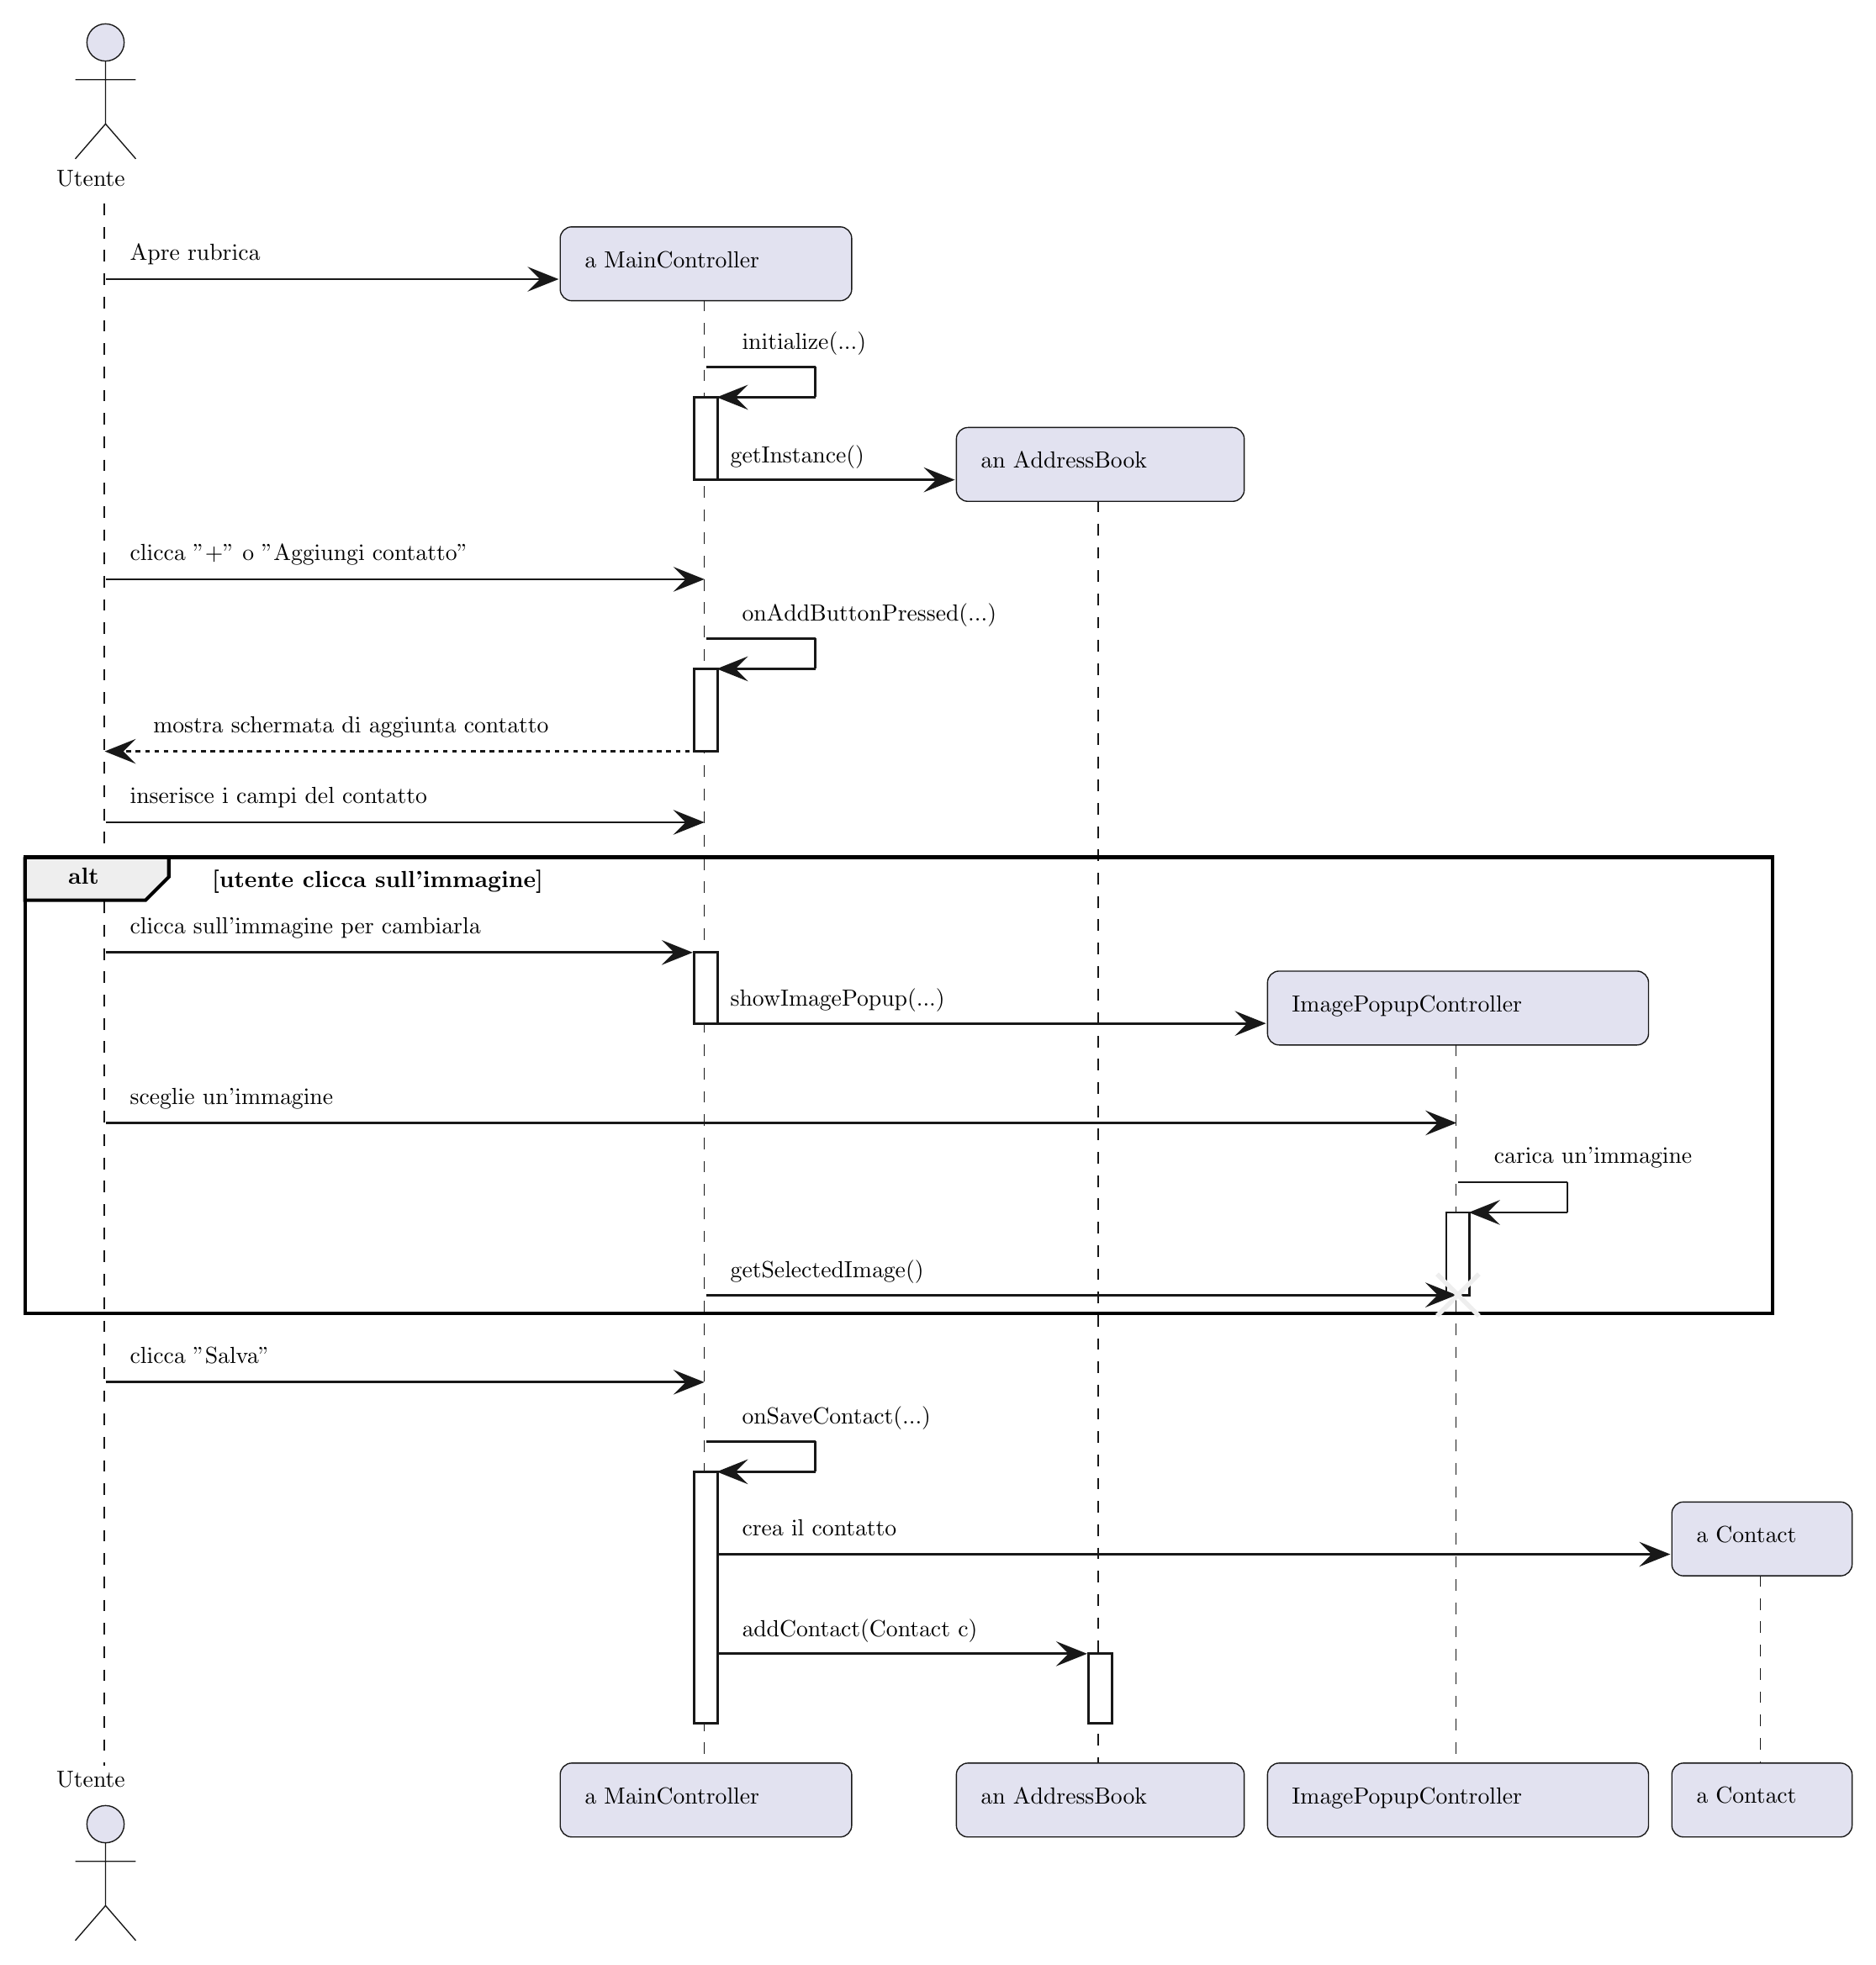
\begin{tikzpicture}[yscale=-1
,pstyle0/.style={color=plantucolor0001,fill=white,line width=1.0pt}
,pstyle1/.style={color=black,line width=1.5pt}
,pstyle2/.style={color=plantucolor0001,line width=0.5pt,dash pattern=on 5.0pt off 5.0pt}
,pstyle3/.style={color=plantucolor0001,fill=plantucolor0003,line width=0.5pt}
,pstyle4/.style={color=plantucolor0001,line width=0.5pt}
,pstyle5/.style={color=plantucolor0001,fill=plantucolor0001,line width=1.0pt}
,pstyle6/.style={color=plantucolor0001,line width=1.0pt}
,pstyle9/.style={color=plantucolor0005,line width=2.0pt}
]
\draw[pstyle0] (297.6157pt,165.9707pt) rectangle (307.6157pt,201.4492pt);
\draw[pstyle0] (297.6157pt,282.6738pt) rectangle (307.6157pt,318.1523pt);
\draw[pstyle0] (297.6157pt,404.5879pt) rectangle (307.6157pt,435.0664pt);
\draw[pstyle0] (297.6157pt,627.7266pt) rectangle (307.6157pt,735.9512pt);
\draw[pstyle0] (467.0763pt,705.9512pt) rectangle (477.0763pt,735.9512pt);
\draw[pstyle0] (620.8057pt,516.291pt) rectangle (630.8057pt,551.7695pt);
\draw[pstyle1] (10pt,363.6309pt) rectangle (761.0057pt,559.7695pt);
\draw[pstyle2] (44pt,82.7461pt) -- (44pt,753.9512pt);
\draw[pstyle2] (301.9816pt,124.1191pt) -- (301.9816pt,753.9512pt);
\draw[pstyle2] (471.2241pt,210.3438pt) -- (471.2241pt,753.9512pt);
\draw[pstyle2] (624.9285pt,443.9609pt) -- (624.9285pt,753.9512pt);
\draw[pstyle2] (755.6828pt,672.0996pt) -- (755.6828pt,753.9512pt);
\node at (20pt,65pt)[below right,color=black]{Utente};
\draw[pstyle3] (44.6pt,13.5pt) ellipse (8pt and 8pt);
\draw[pstyle4] (44.6pt,21.5pt) -- (44.6pt,48.5pt)(31.6pt,29.5pt) -- (57.6pt,29.5pt)(44.6pt,48.5pt) -- (31.6pt,63.5pt)(44.6pt,48.5pt) -- (57.6pt,63.5pt);
\node at (20pt,752.9512pt)[below right,color=black]{Utente};
\draw[pstyle3] (44.6pt,779.1973pt) ellipse (8pt and 8pt);
\draw[pstyle4] (44.6pt,787.1973pt) -- (44.6pt,814.1973pt)(31.6pt,795.1973pt) -- (57.6pt,795.1973pt)(44.6pt,814.1973pt) -- (31.6pt,829.1973pt)(44.6pt,814.1973pt) -- (57.6pt,829.1973pt);
\draw[pstyle3] (239.9816pt,757.9512pt) arc (180:270:5pt) -- (244.9816pt,752.9512pt) -- (360.2497pt,752.9512pt) arc (270:360:5pt) -- (365.2497pt,757.9512pt) -- (365.2497pt,779.6973pt) arc (0:90:5pt) -- (360.2497pt,784.6973pt) -- (244.9816pt,784.6973pt) arc (90:180:5pt) -- (239.9816pt,779.6973pt) -- cycle;
\node at (246.9816pt,759.9512pt)[below right,color=black]{a MainController};
\draw[pstyle3] (410.2241pt,757.9512pt) arc (180:270:5pt) -- (415.2241pt,752.9512pt) -- (528.9285pt,752.9512pt) arc (270:360:5pt) -- (533.9285pt,757.9512pt) -- (533.9285pt,779.6973pt) arc (0:90:5pt) -- (528.9285pt,784.6973pt) -- (415.2241pt,784.6973pt) arc (90:180:5pt) -- (410.2241pt,779.6973pt) -- cycle;
\node at (417.2241pt,759.9512pt)[below right,color=black]{an AddressBook};
\draw[pstyle3] (543.9285pt,757.9512pt) arc (180:270:5pt) -- (548.9285pt,752.9512pt) -- (702.6828pt,752.9512pt) arc (270:360:5pt) -- (707.6828pt,757.9512pt) -- (707.6828pt,779.6973pt) arc (0:90:5pt) -- (702.6828pt,784.6973pt) -- (548.9285pt,784.6973pt) arc (90:180:5pt) -- (543.9285pt,779.6973pt) -- cycle;
\node at (550.9285pt,759.9512pt)[below right,color=black]{ImagePopupController};
\draw[pstyle3] (717.6828pt,757.9512pt) arc (180:270:5pt) -- (722.6828pt,752.9512pt) -- (790.1495pt,752.9512pt) arc (270:360:5pt) -- (795.1495pt,757.9512pt) -- (795.1495pt,779.6973pt) arc (0:90:5pt) -- (790.1495pt,784.6973pt) -- (722.6828pt,784.6973pt) arc (90:180:5pt) -- (717.6828pt,779.6973pt) -- cycle;
\node at (724.6828pt,759.9512pt)[below right,color=black]{a Contact};
\draw[pstyle0] (297.6157pt,165.9707pt) rectangle (307.6157pt,201.4492pt);
\draw[pstyle0] (297.6157pt,282.6738pt) rectangle (307.6157pt,318.1523pt);
\draw[pstyle0] (297.6157pt,404.5879pt) rectangle (307.6157pt,435.0664pt);
\draw[pstyle0] (297.6157pt,627.7266pt) rectangle (307.6157pt,735.9512pt);
\draw[pstyle0] (467.0763pt,705.9512pt) rectangle (477.0763pt,735.9512pt);
\draw[pstyle0] (620.8057pt,516.291pt) rectangle (630.8057pt,551.7695pt);
\draw[pstyle5] (227.9816pt,111.2246pt) -- (237.9816pt,115.2246pt) -- (227.9816pt,119.2246pt) -- (231.9816pt,115.2246pt) -- cycle;
\draw[pstyle6] (44.6pt,115.2246pt) -- (233.9816pt,115.2246pt);
\node at (51.6pt,96.7461pt)[below right,color=black]{Apre rubrica};
\draw[pstyle3] (239.9816pt,97.7461pt) arc (180:270:5pt) -- (244.9816pt,92.7461pt) -- (360.2497pt,92.7461pt) arc (270:360:5pt) -- (365.2497pt,97.7461pt) -- (365.2497pt,119.4922pt) arc (0:90:5pt) -- (360.2497pt,124.4922pt) -- (244.9816pt,124.4922pt) arc (90:180:5pt) -- (239.9816pt,119.4922pt) -- cycle;
\node at (246.9816pt,99.7461pt)[below right,color=black]{a MainController};
\draw[pstyle6] (302.6157pt,152.9707pt) -- (349.6157pt,152.9707pt);
\draw[pstyle6] (349.6157pt,152.9707pt) -- (349.6157pt,165.9707pt);
\draw[pstyle6] (308.6157pt,165.9707pt) -- (349.6157pt,165.9707pt);
\draw[pstyle5] (318.6157pt,161.9707pt) -- (308.6157pt,165.9707pt) -- (318.6157pt,169.9707pt) -- (314.6157pt,165.9707pt) -- cycle;
\node at (314.6157pt,134.4922pt)[below right,color=black]{initialize(...)};
\draw[pstyle5] (398.2241pt,197.4492pt) -- (408.2241pt,201.4492pt) -- (398.2241pt,205.4492pt) -- (402.2241pt,201.4492pt) -- cycle;
\draw[pstyle6] (302.6157pt,201.4492pt) -- (404.2241pt,201.4492pt);
\node at (309.6157pt,182.9707pt)[below right,color=black]{getInstance()};
\draw[pstyle3] (410.2241pt,183.9707pt) arc (180:270:5pt) -- (415.2241pt,178.9707pt) -- (528.9285pt,178.9707pt) arc (270:360:5pt) -- (533.9285pt,183.9707pt) -- (533.9285pt,205.7168pt) arc (0:90:5pt) -- (528.9285pt,210.7168pt) -- (415.2241pt,210.7168pt) arc (90:180:5pt) -- (410.2241pt,205.7168pt) -- cycle;
\node at (417.2241pt,185.9707pt)[below right,color=black]{an AddressBook};
\draw[pstyle5] (290.6157pt,240.1953pt) -- (300.6157pt,244.1953pt) -- (290.6157pt,248.1953pt) -- (294.6157pt,244.1953pt) -- cycle;
\draw[pstyle6] (44.6pt,244.1953pt) -- (296.6157pt,244.1953pt);
\node at (51.6pt,225.7168pt)[below right,color=black]{clicca "+" o "Aggiungi contatto"};
\draw[pstyle6] (302.6157pt,269.6738pt) -- (349.6157pt,269.6738pt);
\draw[pstyle6] (349.6157pt,269.6738pt) -- (349.6157pt,282.6738pt);
\draw[pstyle6] (308.6157pt,282.6738pt) -- (349.6157pt,282.6738pt);
\draw[pstyle5] (318.6157pt,278.6738pt) -- (308.6157pt,282.6738pt) -- (318.6157pt,286.6738pt) -- (314.6157pt,282.6738pt) -- cycle;
\node at (314.6157pt,251.1953pt)[below right,color=black]{onAddButtonPressed(...)};
\draw[pstyle5] (55.6pt,314.1523pt) -- (45.6pt,318.1523pt) -- (55.6pt,322.1523pt) -- (51.6pt,318.1523pt) -- cycle;
\draw[color=plantucolor0001,line width=1.0pt,dash pattern=on 2.0pt off 2.0pt] (49.6pt,318.1523pt) -- (301.6157pt,318.1523pt);
\node at (61.6pt,299.6738pt)[below right,color=black]{mostra schermata di aggiunta contatto};
\draw[pstyle5] (290.6157pt,344.6309pt) -- (300.6157pt,348.6309pt) -- (290.6157pt,352.6309pt) -- (294.6157pt,348.6309pt) -- cycle;
\draw[pstyle6] (44.6pt,348.6309pt) -- (296.6157pt,348.6309pt);
\node at (51.6pt,330.1523pt)[below right,color=black]{inserisce i campi del contatto};
\draw[color=black,fill=plantucolor0004,line width=1.5pt] (10pt,363.6309pt) -- (71.8pt,363.6309pt) -- (71.8pt,372.1094pt) -- (61.8pt,382.1094pt) -- (10pt,382.1094pt) -- (10pt,363.6309pt);
\draw[pstyle1] (10pt,363.6309pt) rectangle (761.0057pt,559.7695pt);
\node at (25pt,364.6309pt)[below right,color=black]{\textbf{alt}};
\node at (86.8pt,365.6309pt)[below right,color=black]{\textbf{[utente clicca sull'immagine]}};
\draw[pstyle5] (285.6157pt,400.5879pt) -- (295.6157pt,404.5879pt) -- (285.6157pt,408.5879pt) -- (289.6157pt,404.5879pt) -- cycle;
\draw[pstyle6] (44.6pt,404.5879pt) -- (291.6157pt,404.5879pt);
\node at (51.6pt,386.1094pt)[below right,color=black]{clicca sull'immagine per cambiarla};
\draw[pstyle5] (531.9285pt,431.0664pt) -- (541.9285pt,435.0664pt) -- (531.9285pt,439.0664pt) -- (535.9285pt,435.0664pt) -- cycle;
\draw[pstyle6] (302.6157pt,435.0664pt) -- (537.9285pt,435.0664pt);
\node at (309.6157pt,416.5879pt)[below right,color=black]{showImagePopup(...)};
\draw[pstyle3] (543.9285pt,417.5879pt) arc (180:270:5pt) -- (548.9285pt,412.5879pt) -- (702.6828pt,412.5879pt) arc (270:360:5pt) -- (707.6828pt,417.5879pt) -- (707.6828pt,439.334pt) arc (0:90:5pt) -- (702.6828pt,444.334pt) -- (548.9285pt,444.334pt) arc (90:180:5pt) -- (543.9285pt,439.334pt) -- cycle;
\node at (550.9285pt,419.5879pt)[below right,color=black]{ImagePopupController};
\draw[pstyle5] (613.8057pt,473.8125pt) -- (623.8057pt,477.8125pt) -- (613.8057pt,481.8125pt) -- (617.8057pt,477.8125pt) -- cycle;
\draw[pstyle6] (44.6pt,477.8125pt) -- (619.8057pt,477.8125pt);
\node at (51.6pt,459.334pt)[below right,color=black]{sceglie un'immagine};
\draw[pstyle6] (625.8057pt,503.291pt) -- (672.8057pt,503.291pt);
\draw[pstyle6] (672.8057pt,503.291pt) -- (672.8057pt,516.291pt);
\draw[pstyle6] (631.8057pt,516.291pt) -- (672.8057pt,516.291pt);
\draw[pstyle5] (641.8057pt,512.291pt) -- (631.8057pt,516.291pt) -- (641.8057pt,520.291pt) -- (637.8057pt,516.291pt) -- cycle;
\node at (637.8057pt,484.8125pt)[below right,color=black]{carica un'immagine};
\draw[pstyle5] (613.8057pt,547.7695pt) -- (623.8057pt,551.7695pt) -- (613.8057pt,555.7695pt) -- (617.8057pt,551.7695pt) -- cycle;
\draw[pstyle6] (302.6157pt,551.7695pt) -- (619.8057pt,551.7695pt);
\node at (309.6157pt,533.291pt)[below right,color=black]{getSelectedImage()};
\draw[pstyle9] (616.8057pt,542.7695pt) -- (634.8057pt,560.7695pt);
\draw[pstyle9] (616.8057pt,560.7695pt) -- (634.8057pt,542.7695pt);
\draw[pstyle5] (290.6157pt,585.248pt) -- (300.6157pt,589.248pt) -- (290.6157pt,593.248pt) -- (294.6157pt,589.248pt) -- cycle;
\draw[pstyle6] (44.6pt,589.248pt) -- (296.6157pt,589.248pt);
\node at (51.6pt,570.7695pt)[below right,color=black]{clicca "Salva"};
\draw[pstyle6] (302.6157pt,614.7266pt) -- (349.6157pt,614.7266pt);
\draw[pstyle6] (349.6157pt,614.7266pt) -- (349.6157pt,627.7266pt);
\draw[pstyle6] (308.6157pt,627.7266pt) -- (349.6157pt,627.7266pt);
\draw[pstyle5] (318.6157pt,623.7266pt) -- (308.6157pt,627.7266pt) -- (318.6157pt,631.7266pt) -- (314.6157pt,627.7266pt) -- cycle;
\node at (314.6157pt,596.248pt)[below right,color=black]{onSaveContact(...)};
\draw[pstyle5] (705.6828pt,659.2051pt) -- (715.6828pt,663.2051pt) -- (705.6828pt,667.2051pt) -- (709.6828pt,663.2051pt) -- cycle;
\draw[pstyle6] (307.6157pt,663.2051pt) -- (711.6828pt,663.2051pt);
\node at (314.6157pt,644.7266pt)[below right,color=black]{crea il contatto};
\draw[pstyle3] (717.6828pt,645.7266pt) arc (180:270:5pt) -- (722.6828pt,640.7266pt) -- (790.1495pt,640.7266pt) arc (270:360:5pt) -- (795.1495pt,645.7266pt) -- (795.1495pt,667.4727pt) arc (0:90:5pt) -- (790.1495pt,672.4727pt) -- (722.6828pt,672.4727pt) arc (90:180:5pt) -- (717.6828pt,667.4727pt) -- cycle;
\node at (724.6828pt,647.7266pt)[below right,color=black]{a Contact};
\draw[pstyle5] (455.0763pt,701.9512pt) -- (465.0763pt,705.9512pt) -- (455.0763pt,709.9512pt) -- (459.0763pt,705.9512pt) -- cycle;
\draw[pstyle6] (307.6157pt,705.9512pt) -- (461.0763pt,705.9512pt);
\node at (314.6157pt,687.4727pt)[below right,color=black]{addContact(Contact c)};
\end{tikzpicture}
}
\end{adjustbox}

\begin{figure}[h]
\caption{Diagramma sequenza C1 - Aggiungere Contatto}
\label{fig:Diagramma sequenza C1 - Aggiungere Contatto}
\end{figure}

\newpage
\subsubsection{C2 C3 - Eliminare Modificare Contatto}
Il seguente diagramma di sequenza illustra l'esecuzione di entrambi i casi d'uso C2 e C3, tramite la sintassi \texttt{loop}, \texttt{break} e \texttt{alt}:
% generated by Plantuml 1.2024.3       
\definecolor{plantucolor0000}{RGB}{255,255,255}
\definecolor{plantucolor0001}{RGB}{24,24,24}
\definecolor{plantucolor0002}{RGB}{0,0,0}
\definecolor{plantucolor0003}{RGB}{226,226,240}
\definecolor{plantucolor0004}{RGB}{238,238,238}

\begin{adjustbox}{width=.84\paperwidth, center}
	\resizebox{\textwidth}{!}{
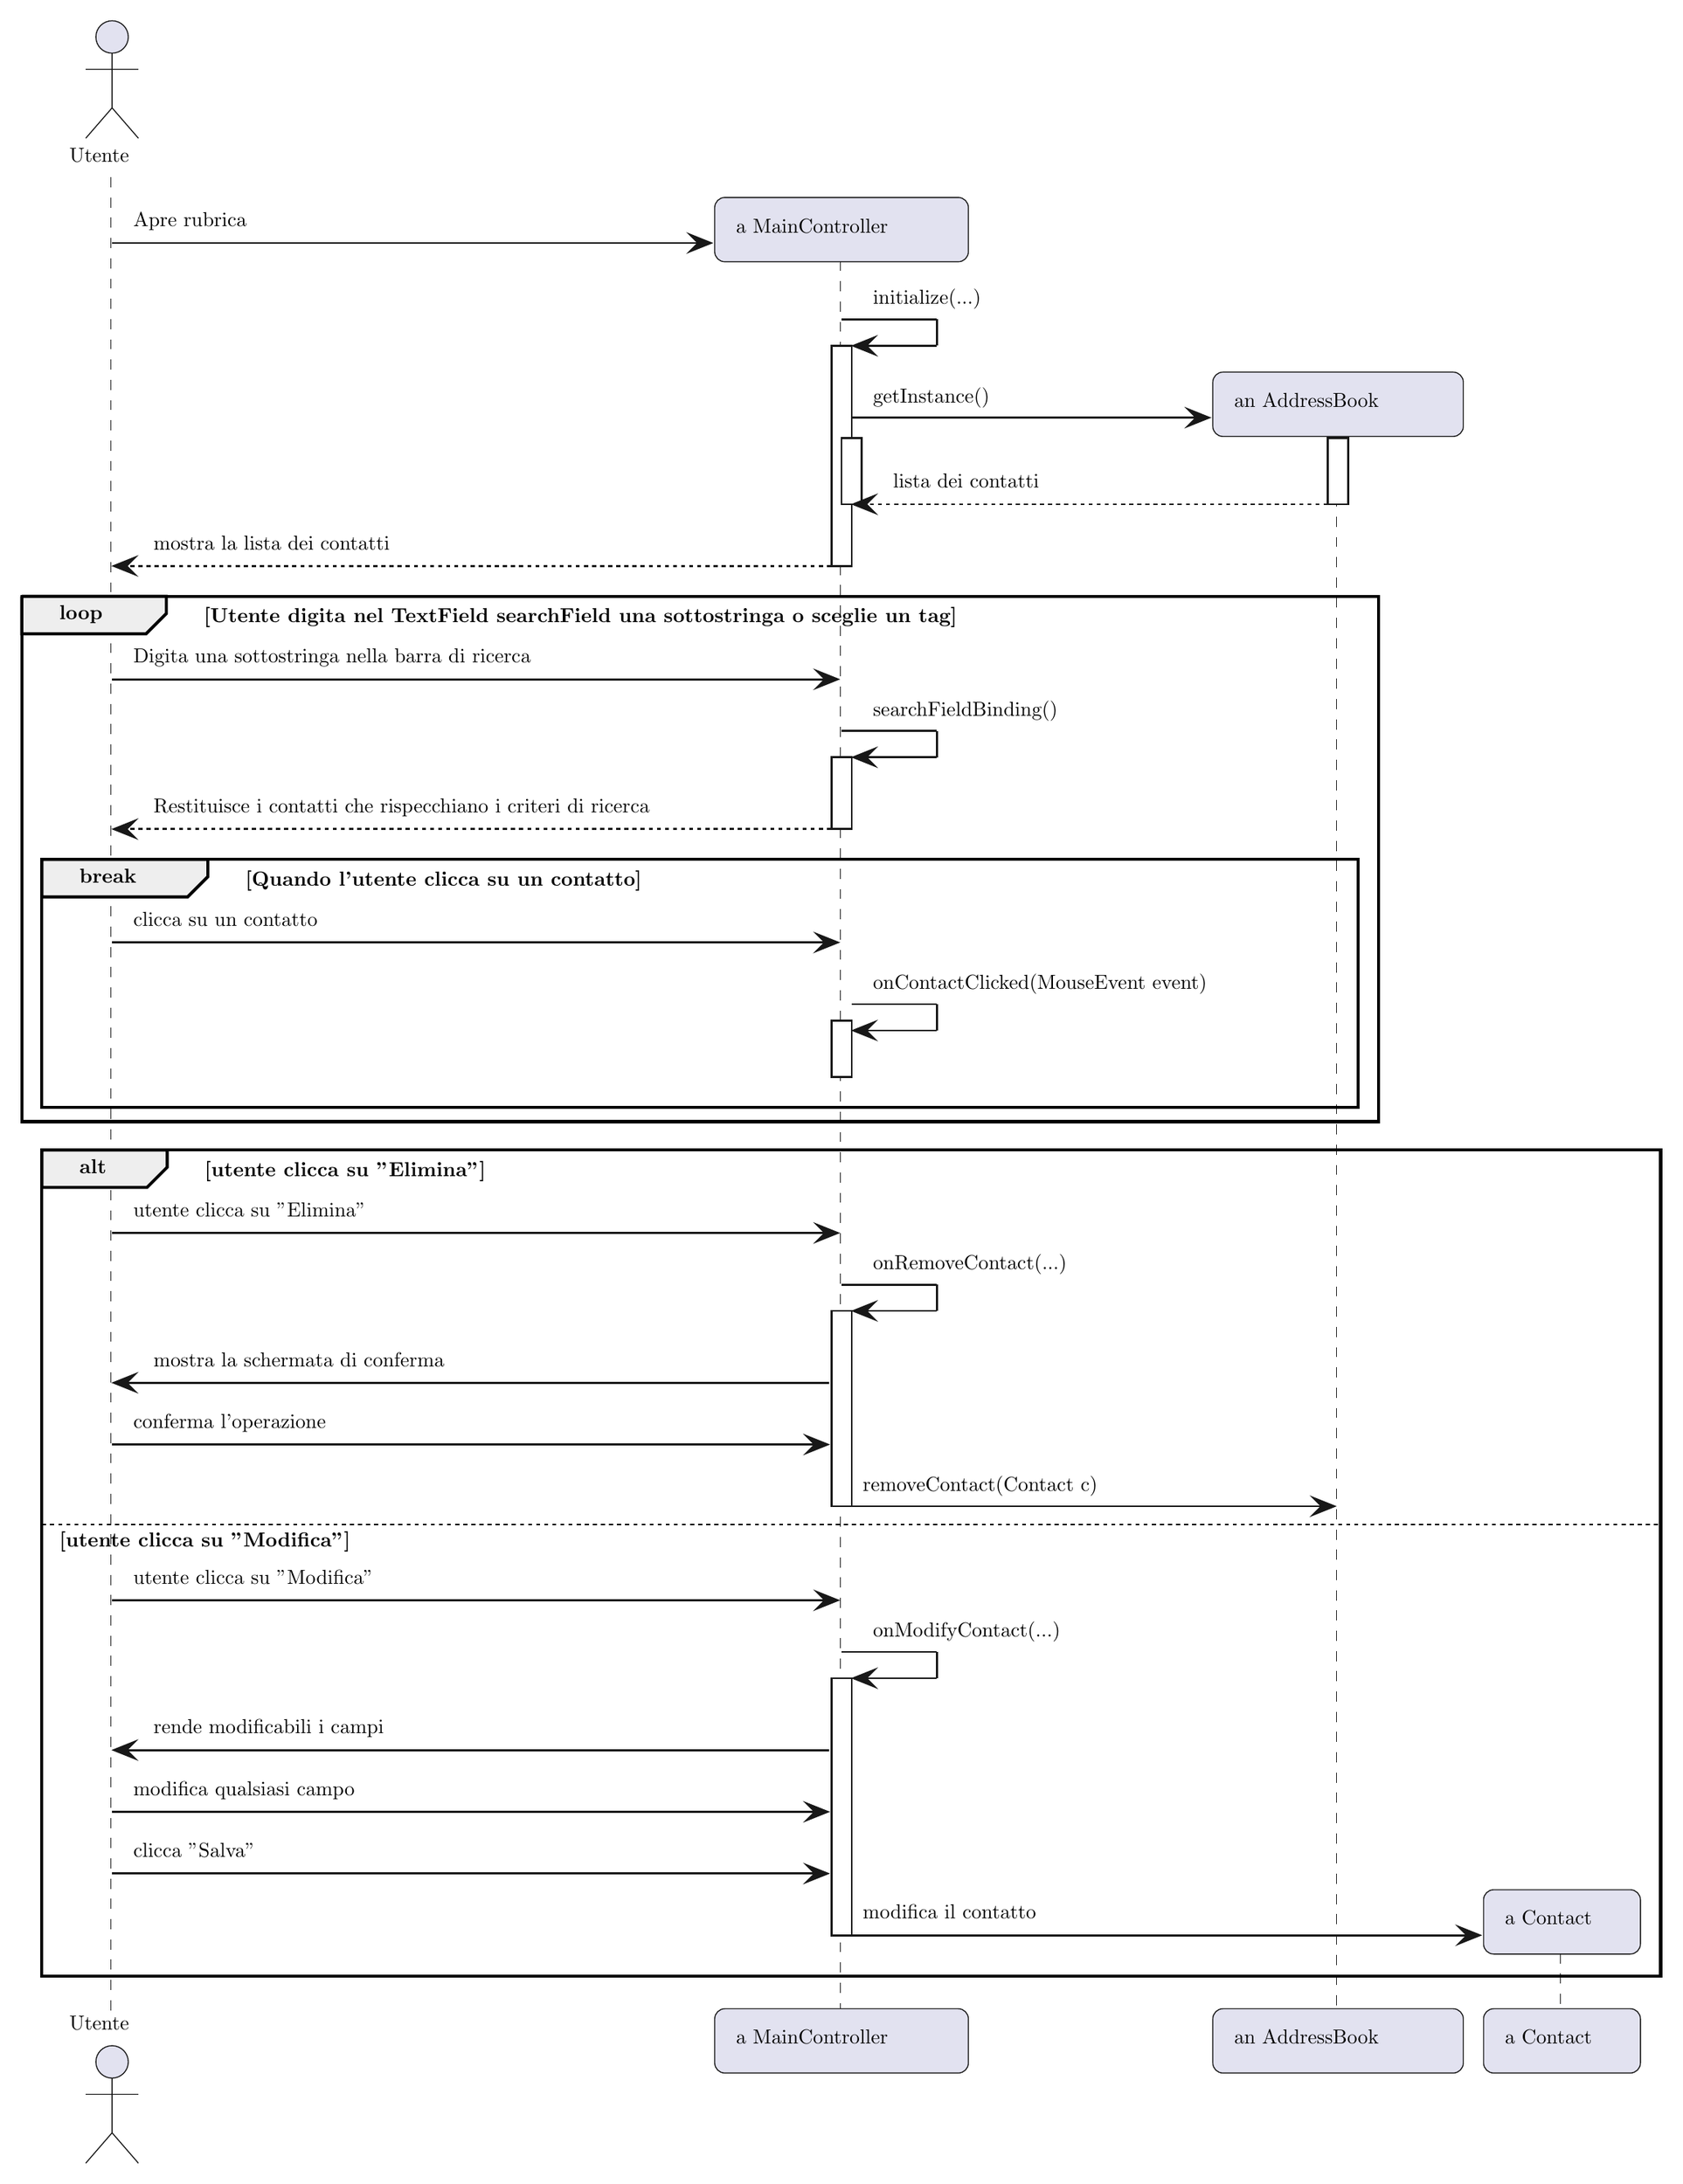
\begin{tikzpicture}[yscale=-1
,pstyle0/.style={color=plantucolor0001,fill=white,line width=1.0pt}
,pstyle1/.style={color=black,line width=1.5pt}
,pstyle2/.style={color=plantucolor0001,line width=0.5pt,dash pattern=on 5.0pt off 5.0pt}
,pstyle3/.style={color=plantucolor0001,fill=plantucolor0003,line width=0.5pt}
,pstyle4/.style={color=plantucolor0001,line width=0.5pt}
,pstyle5/.style={color=plantucolor0001,fill=plantucolor0001,line width=1.0pt}
,pstyle6/.style={color=plantucolor0001,line width=1.0pt}
,pstyle7/.style={color=plantucolor0001,line width=1.0pt,dash pattern=on 2.0pt off 2.0pt}
,pstyle8/.style={color=black,fill=plantucolor0004,line width=1.5pt}
]
\draw[pstyle0] (409.8219pt,165.9707pt) rectangle (419.8219pt,274.6738pt);
\draw[pstyle0] (414.8219pt,211.4492pt) rectangle (424.8219pt,244.1953pt);
\draw[pstyle0] (409.8219pt,369.1094pt) rectangle (419.8219pt,404.5879pt);
\draw[pstyle0] (409.8219pt,499.0234pt) rectangle (419.8219pt,527.0234pt);
\draw[pstyle0] (409.8219pt,642.459pt) rectangle (419.8219pt,738.8945pt);
\draw[pstyle0] (409.8219pt,823.7949pt) rectangle (419.8219pt,950.709pt);
\draw[pstyle0] (655.0081pt,211.4492pt) rectangle (665.0081pt,244.1953pt);
\draw[pstyle1] (10pt,289.6738pt) rectangle (680.0081pt,549.0234pt);
\draw[pstyle1] (20pt,419.5879pt) rectangle (670.0081pt,542.0234pt);
\draw[pstyle1] (20pt,563.0234pt) rectangle (819.327pt,970.9766pt);
\draw[pstyle2] (54pt,82.7461pt) -- (54pt,987.9766pt);
\draw[pstyle2] (414.1879pt,124.1191pt) -- (414.1879pt,987.9766pt);
\draw[pstyle2] (659.156pt,210.3438pt) -- (659.156pt,987.9766pt);
\draw[pstyle2] (769.8603pt,959.6035pt) -- (769.8603pt,987.9766pt);
\node at (30pt,65pt)[below right,color=black]{Utente};
\draw[pstyle3] (54.6pt,13.5pt) ellipse (8pt and 8pt);
\draw[pstyle4] (54.6pt,21.5pt) -- (54.6pt,48.5pt)(41.6pt,29.5pt) -- (67.6pt,29.5pt)(54.6pt,48.5pt) -- (41.6pt,63.5pt)(54.6pt,48.5pt) -- (67.6pt,63.5pt);
\node at (30pt,986.9766pt)[below right,color=black]{Utente};
\draw[pstyle3] (54.6pt,1013.2227pt) ellipse (8pt and 8pt);
\draw[pstyle4] (54.6pt,1021.2227pt) -- (54.6pt,1048.2227pt)(41.6pt,1029.2227pt) -- (67.6pt,1029.2227pt)(54.6pt,1048.2227pt) -- (41.6pt,1063.2227pt)(54.6pt,1048.2227pt) -- (67.6pt,1063.2227pt);
\draw[pstyle3] (352.1879pt,991.9766pt) arc (180:270:5pt) -- (357.1879pt,986.9766pt) -- (472.456pt,986.9766pt) arc (270:360:5pt) -- (477.456pt,991.9766pt) -- (477.456pt,1013.7227pt) arc (0:90:5pt) -- (472.456pt,1018.7227pt) -- (357.1879pt,1018.7227pt) arc (90:180:5pt) -- (352.1879pt,1013.7227pt) -- cycle;
\node at (359.1879pt,993.9766pt)[below right,color=black]{a MainController};
\draw[pstyle3] (598.156pt,991.9766pt) arc (180:270:5pt) -- (603.156pt,986.9766pt) -- (716.8603pt,986.9766pt) arc (270:360:5pt) -- (721.8603pt,991.9766pt) -- (721.8603pt,1013.7227pt) arc (0:90:5pt) -- (716.8603pt,1018.7227pt) -- (603.156pt,1018.7227pt) arc (90:180:5pt) -- (598.156pt,1013.7227pt) -- cycle;
\node at (605.156pt,993.9766pt)[below right,color=black]{an AddressBook};
\draw[pstyle3] (731.8603pt,991.9766pt) arc (180:270:5pt) -- (736.8603pt,986.9766pt) -- (804.327pt,986.9766pt) arc (270:360:5pt) -- (809.327pt,991.9766pt) -- (809.327pt,1013.7227pt) arc (0:90:5pt) -- (804.327pt,1018.7227pt) -- (736.8603pt,1018.7227pt) arc (90:180:5pt) -- (731.8603pt,1013.7227pt) -- cycle;
\node at (738.8603pt,993.9766pt)[below right,color=black]{a Contact};
\draw[pstyle0] (409.8219pt,165.9707pt) rectangle (419.8219pt,274.6738pt);
\draw[pstyle0] (414.8219pt,211.4492pt) rectangle (424.8219pt,244.1953pt);
\draw[pstyle0] (409.8219pt,369.1094pt) rectangle (419.8219pt,404.5879pt);
\draw[pstyle0] (409.8219pt,499.0234pt) rectangle (419.8219pt,527.0234pt);
\draw[pstyle0] (409.8219pt,642.459pt) rectangle (419.8219pt,738.8945pt);
\draw[pstyle0] (409.8219pt,823.7949pt) rectangle (419.8219pt,950.709pt);
\draw[pstyle0] (655.0081pt,211.4492pt) rectangle (665.0081pt,244.1953pt);
\draw[pstyle5] (340.1879pt,111.2246pt) -- (350.1879pt,115.2246pt) -- (340.1879pt,119.2246pt) -- (344.1879pt,115.2246pt) -- cycle;
\draw[pstyle6] (54.6pt,115.2246pt) -- (346.1879pt,115.2246pt);
\node at (61.6pt,96.7461pt)[below right,color=black]{Apre rubrica};
\draw[pstyle3] (352.1879pt,97.7461pt) arc (180:270:5pt) -- (357.1879pt,92.7461pt) -- (472.456pt,92.7461pt) arc (270:360:5pt) -- (477.456pt,97.7461pt) -- (477.456pt,119.4922pt) arc (0:90:5pt) -- (472.456pt,124.4922pt) -- (357.1879pt,124.4922pt) arc (90:180:5pt) -- (352.1879pt,119.4922pt) -- cycle;
\node at (359.1879pt,99.7461pt)[below right,color=black]{a MainController};
\draw[pstyle6] (414.8219pt,152.9707pt) -- (461.8219pt,152.9707pt);
\draw[pstyle6] (461.8219pt,152.9707pt) -- (461.8219pt,165.9707pt);
\draw[pstyle6] (420.8219pt,165.9707pt) -- (461.8219pt,165.9707pt);
\draw[pstyle5] (430.8219pt,161.9707pt) -- (420.8219pt,165.9707pt) -- (430.8219pt,169.9707pt) -- (426.8219pt,165.9707pt) -- cycle;
\node at (426.8219pt,134.4922pt)[below right,color=black]{initialize(...)};
\draw[pstyle5] (586.156pt,197.4492pt) -- (596.156pt,201.4492pt) -- (586.156pt,205.4492pt) -- (590.156pt,201.4492pt) -- cycle;
\draw[pstyle6] (419.8219pt,201.4492pt) -- (592.156pt,201.4492pt);
\node at (426.8219pt,182.9707pt)[below right,color=black]{getInstance()};
\draw[pstyle3] (598.156pt,183.9707pt) arc (180:270:5pt) -- (603.156pt,178.9707pt) -- (716.8603pt,178.9707pt) arc (270:360:5pt) -- (721.8603pt,183.9707pt) -- (721.8603pt,205.7168pt) arc (0:90:5pt) -- (716.8603pt,210.7168pt) -- (603.156pt,210.7168pt) arc (90:180:5pt) -- (598.156pt,205.7168pt) -- cycle;
\node at (605.156pt,185.9707pt)[below right,color=black]{an AddressBook};
\draw[pstyle5] (430.8219pt,240.1953pt) -- (420.8219pt,244.1953pt) -- (430.8219pt,248.1953pt) -- (426.8219pt,244.1953pt) -- cycle;
\draw[pstyle7] (424.8219pt,244.1953pt) -- (659.0081pt,244.1953pt);
\node at (436.8219pt,225.7168pt)[below right,color=black]{lista dei contatti};
\draw[pstyle5] (65.6pt,270.6738pt) -- (55.6pt,274.6738pt) -- (65.6pt,278.6738pt) -- (61.6pt,274.6738pt) -- cycle;
\draw[pstyle7] (59.6pt,274.6738pt) -- (413.8219pt,274.6738pt);
\node at (71.6pt,256.1953pt)[below right,color=black]{mostra la lista dei contatti};
\draw[pstyle8] (10pt,289.6738pt) -- (81.4pt,289.6738pt) -- (81.4pt,298.1523pt) -- (71.4pt,308.1523pt) -- (10pt,308.1523pt) -- (10pt,289.6738pt);
\draw[pstyle1] (10pt,289.6738pt) rectangle (680.0081pt,549.0234pt);
\node at (25pt,290.6738pt)[below right,color=black]{\textbf{loop}};
\node at (96.4pt,291.6738pt)[below right,color=black]{\textbf{[Utente digita nel TextField searchField una sottostringa o sceglie un tag]}};
\draw[pstyle5] (402.8219pt,326.6309pt) -- (412.8219pt,330.6309pt) -- (402.8219pt,334.6309pt) -- (406.8219pt,330.6309pt) -- cycle;
\draw[pstyle6] (54.6pt,330.6309pt) -- (408.8219pt,330.6309pt);
\node at (61.6pt,312.1523pt)[below right,color=black]{Digita una sottostringa nella barra di ricerca};
\draw[pstyle6] (414.8219pt,356.1094pt) -- (461.8219pt,356.1094pt);
\draw[pstyle6] (461.8219pt,356.1094pt) -- (461.8219pt,369.1094pt);
\draw[pstyle6] (420.8219pt,369.1094pt) -- (461.8219pt,369.1094pt);
\draw[pstyle5] (430.8219pt,365.1094pt) -- (420.8219pt,369.1094pt) -- (430.8219pt,373.1094pt) -- (426.8219pt,369.1094pt) -- cycle;
\node at (426.8219pt,337.6309pt)[below right,color=black]{searchFieldBinding()};
\draw[pstyle5] (65.6pt,400.5879pt) -- (55.6pt,404.5879pt) -- (65.6pt,408.5879pt) -- (61.6pt,404.5879pt) -- cycle;
\draw[pstyle7] (59.6pt,404.5879pt) -- (413.8219pt,404.5879pt);
\node at (71.6pt,386.1094pt)[below right,color=black]{Restituisce i contatti che rispecchiano i criteri di ricerca};
\draw[pstyle8] (20pt,419.5879pt) -- (101.9pt,419.5879pt) -- (101.9pt,428.0664pt) -- (91.9pt,438.0664pt) -- (20pt,438.0664pt) -- (20pt,419.5879pt);
\draw[pstyle1] (20pt,419.5879pt) rectangle (670.0081pt,542.0234pt);
\node at (35pt,420.5879pt)[below right,color=black]{\textbf{break}};
\node at (116.9pt,421.5879pt)[below right,color=black]{\textbf{[Quando l'utente clicca su un contatto]}};
\draw[pstyle5] (402.8219pt,456.5449pt) -- (412.8219pt,460.5449pt) -- (402.8219pt,464.5449pt) -- (406.8219pt,460.5449pt) -- cycle;
\draw[pstyle6] (54.6pt,460.5449pt) -- (408.8219pt,460.5449pt);
\node at (61.6pt,442.0664pt)[below right,color=black]{clicca su un contatto};
\draw[pstyle6] (419.8219pt,491.0234pt) -- (461.8219pt,491.0234pt);
\draw[pstyle6] (461.8219pt,491.0234pt) -- (461.8219pt,504.0234pt);
\draw[pstyle6] (420.8219pt,504.0234pt) -- (461.8219pt,504.0234pt);
\draw[pstyle5] (430.8219pt,500.0234pt) -- (420.8219pt,504.0234pt) -- (430.8219pt,508.0234pt) -- (426.8219pt,504.0234pt) -- cycle;
\node at (426.8219pt,472.5449pt)[below right,color=black]{onContactClicked(MouseEvent event)};
\draw[pstyle8] (20pt,563.0234pt) -- (81.8pt,563.0234pt) -- (81.8pt,571.502pt) -- (71.8pt,581.502pt) -- (20pt,581.502pt) -- (20pt,563.0234pt);
\draw[pstyle1] (20pt,563.0234pt) rectangle (819.327pt,970.9766pt);
\node at (35pt,564.0234pt)[below right,color=black]{\textbf{alt}};
\node at (96.8pt,565.0234pt)[below right,color=black]{\textbf{[utente clicca su "Elimina"]}};
\draw[pstyle5] (402.8219pt,599.9805pt) -- (412.8219pt,603.9805pt) -- (402.8219pt,607.9805pt) -- (406.8219pt,603.9805pt) -- cycle;
\draw[pstyle6] (54.6pt,603.9805pt) -- (408.8219pt,603.9805pt);
\node at (61.6pt,585.502pt)[below right,color=black]{utente clicca su "Elimina"};
\draw[pstyle6] (414.8219pt,629.459pt) -- (461.8219pt,629.459pt);
\draw[pstyle6] (461.8219pt,629.459pt) -- (461.8219pt,642.459pt);
\draw[pstyle6] (420.8219pt,642.459pt) -- (461.8219pt,642.459pt);
\draw[pstyle5] (430.8219pt,638.459pt) -- (420.8219pt,642.459pt) -- (430.8219pt,646.459pt) -- (426.8219pt,642.459pt) -- cycle;
\node at (426.8219pt,610.9805pt)[below right,color=black]{onRemoveContact(...)};
\draw[pstyle5] (65.6pt,673.9375pt) -- (55.6pt,677.9375pt) -- (65.6pt,681.9375pt) -- (61.6pt,677.9375pt) -- cycle;
\draw[pstyle6] (59.6pt,677.9375pt) -- (408.8219pt,677.9375pt);
\node at (71.6pt,659.459pt)[below right,color=black]{mostra la schermata di conferma};
\draw[pstyle5] (397.8219pt,704.416pt) -- (407.8219pt,708.416pt) -- (397.8219pt,712.416pt) -- (401.8219pt,708.416pt) -- cycle;
\draw[pstyle6] (54.6pt,708.416pt) -- (403.8219pt,708.416pt);
\node at (61.6pt,689.9375pt)[below right,color=black]{conferma l'operazione};
\draw[pstyle5] (648.0081pt,734.8945pt) -- (658.0081pt,738.8945pt) -- (648.0081pt,742.8945pt) -- (652.0081pt,738.8945pt) -- cycle;
\draw[pstyle6] (414.8219pt,738.8945pt) -- (654.0081pt,738.8945pt);
\node at (421.8219pt,720.416pt)[below right,color=black]{removeContact(Contact c)};
\draw[color=black,line width=1.0pt,dash pattern=on 2.0pt off 2.0pt] (20pt,747.8945pt) -- (819.327pt,747.8945pt);
\node at (25pt,747.8945pt)[below right,color=black]{\textbf{[utente clicca su "Modifica"]}};
\draw[pstyle5] (402.8219pt,781.3164pt) -- (412.8219pt,785.3164pt) -- (402.8219pt,789.3164pt) -- (406.8219pt,785.3164pt) -- cycle;
\draw[pstyle6] (54.6pt,785.3164pt) -- (408.8219pt,785.3164pt);
\node at (61.6pt,766.8379pt)[below right,color=black]{utente clicca su "Modifica"};
\draw[pstyle6] (414.8219pt,810.7949pt) -- (461.8219pt,810.7949pt);
\draw[pstyle6] (461.8219pt,810.7949pt) -- (461.8219pt,823.7949pt);
\draw[pstyle6] (420.8219pt,823.7949pt) -- (461.8219pt,823.7949pt);
\draw[pstyle5] (430.8219pt,819.7949pt) -- (420.8219pt,823.7949pt) -- (430.8219pt,827.7949pt) -- (426.8219pt,823.7949pt) -- cycle;
\node at (426.8219pt,792.3164pt)[below right,color=black]{onModifyContact(...)};
\draw[pstyle5] (65.6pt,855.2734pt) -- (55.6pt,859.2734pt) -- (65.6pt,863.2734pt) -- (61.6pt,859.2734pt) -- cycle;
\draw[pstyle6] (59.6pt,859.2734pt) -- (408.8219pt,859.2734pt);
\node at (71.6pt,840.7949pt)[below right,color=black]{rende modificabili i campi};
\draw[pstyle5] (397.8219pt,885.752pt) -- (407.8219pt,889.752pt) -- (397.8219pt,893.752pt) -- (401.8219pt,889.752pt) -- cycle;
\draw[pstyle6] (54.6pt,889.752pt) -- (403.8219pt,889.752pt);
\node at (61.6pt,871.2734pt)[below right,color=black]{modifica qualsiasi campo};
\draw[pstyle5] (397.8219pt,916.2305pt) -- (407.8219pt,920.2305pt) -- (397.8219pt,924.2305pt) -- (401.8219pt,920.2305pt) -- cycle;
\draw[pstyle6] (54.6pt,920.2305pt) -- (403.8219pt,920.2305pt);
\node at (61.6pt,901.752pt)[below right,color=black]{clicca "Salva"};
\draw[pstyle5] (719.8603pt,946.709pt) -- (729.8603pt,950.709pt) -- (719.8603pt,954.709pt) -- (723.8603pt,950.709pt) -- cycle;
\draw[pstyle6] (414.8219pt,950.709pt) -- (725.8603pt,950.709pt);
\node at (421.8219pt,932.2305pt)[below right,color=black]{modifica il contatto};
\draw[pstyle3] (731.8603pt,933.2305pt) arc (180:270:5pt) -- (736.8603pt,928.2305pt) -- (804.327pt,928.2305pt) arc (270:360:5pt) -- (809.327pt,933.2305pt) -- (809.327pt,954.9766pt) arc (0:90:5pt) -- (804.327pt,959.9766pt) -- (736.8603pt,959.9766pt) arc (90:180:5pt) -- (731.8603pt,954.9766pt) -- cycle;
\node at (738.8603pt,935.2305pt)[below right,color=black]{a Contact};
\end{tikzpicture}
}
\end{adjustbox}
\begin{figure}[h]
\caption{Diagramma sequenza C2 C3 - Eliminare Modificare Contatto}
\label{fig:Diagramma sequenza C2 C3 - Eliminare Modificare Contatto}
\end{figure}

\newpage
\subsubsection{C5 - Importare rubrica}
Il seguente diagramma di sequenza illustra l'esecuzione del caso d'uso C5:
% generated by Plantuml 1.2024.3       
\definecolor{plantucolor0000}{RGB}{255,255,255}
\definecolor{plantucolor0001}{RGB}{24,24,24}
\definecolor{plantucolor0002}{RGB}{0,0,0}
\definecolor{plantucolor0003}{RGB}{226,226,240}
\definecolor{plantucolor0004}{RGB}{238,238,238}
\definecolor{plantucolor0005}{RGB}{168,0,54}

\begin{adjustbox}{width=.9\paperwidth, center}
	\resizebox{\textwidth}{!}{
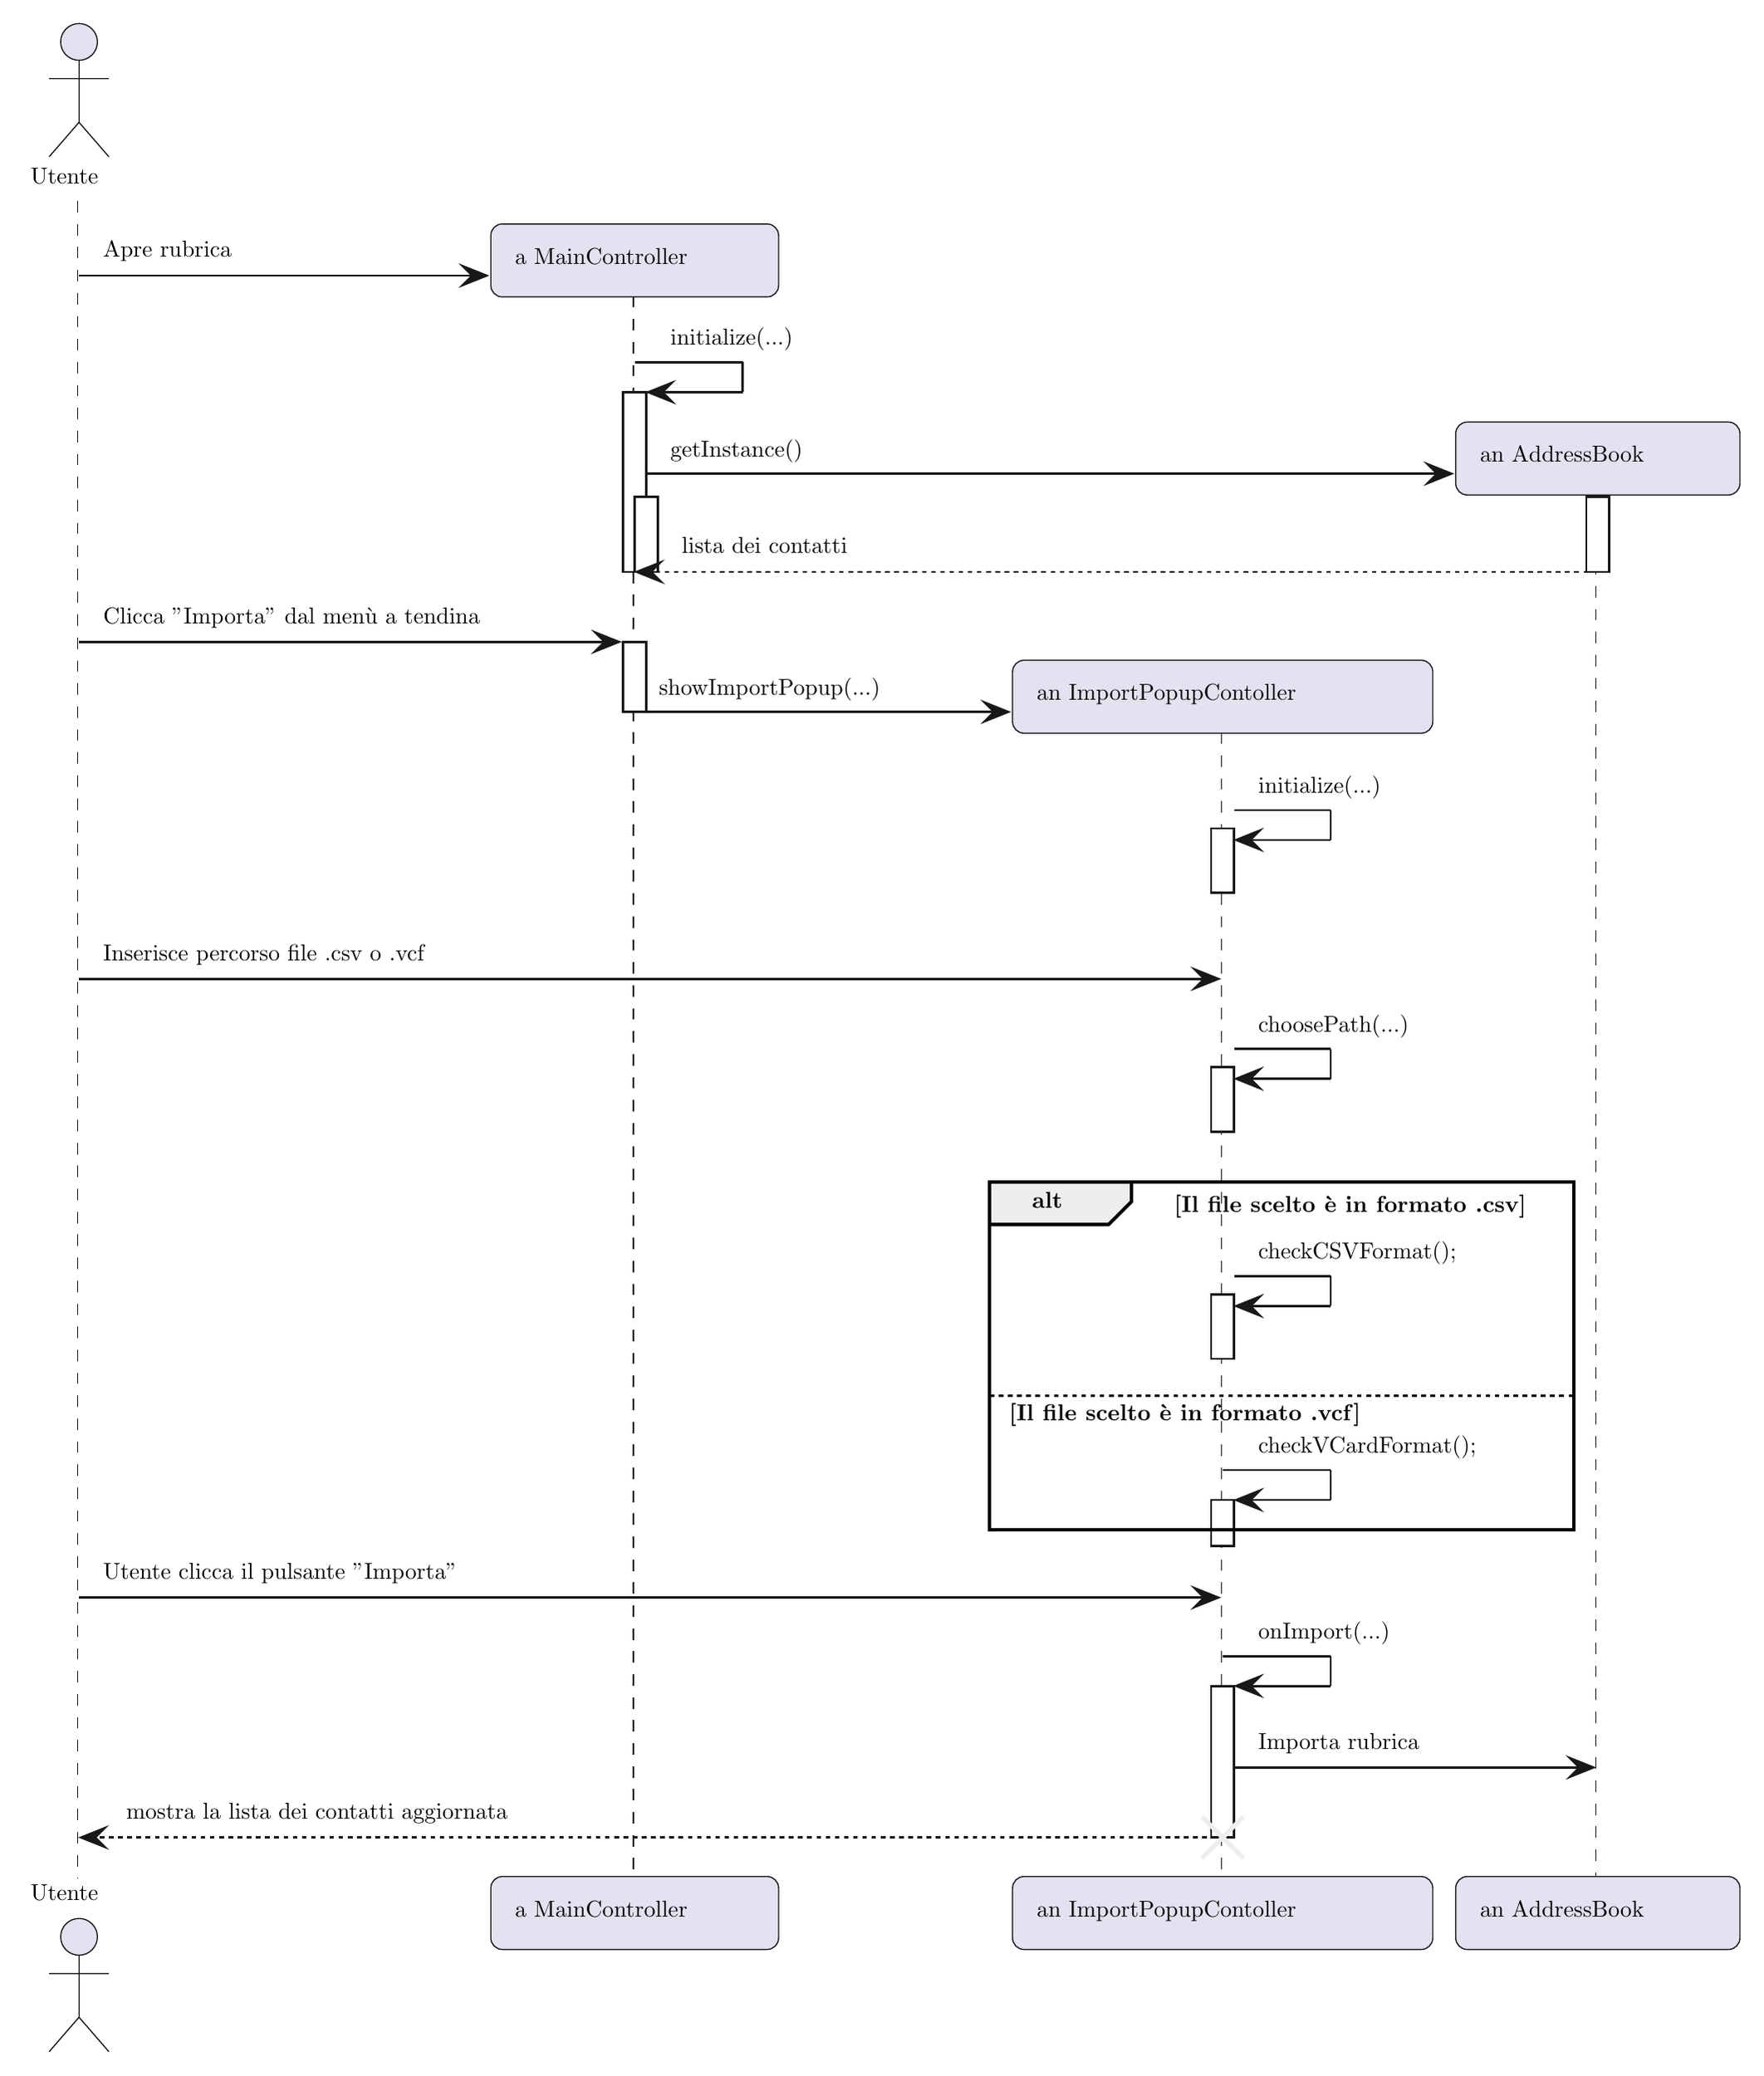
\begin{tikzpicture}[yscale=-1
,pstyle0/.style={color=plantucolor0001,fill=white,line width=1.0pt}
,pstyle1/.style={color=black,line width=1.5pt}
,pstyle2/.style={color=plantucolor0001,line width=0.5pt,dash pattern=on 5.0pt off 5.0pt}
,pstyle3/.style={color=plantucolor0001,fill=plantucolor0003,line width=0.5pt}
,pstyle4/.style={color=plantucolor0001,line width=0.5pt}
,pstyle5/.style={color=plantucolor0001,fill=plantucolor0001,line width=1.0pt}
,pstyle6/.style={color=plantucolor0001,line width=1.0pt}
,pstyle7/.style={color=plantucolor0001,line width=1.0pt,dash pattern=on 2.0pt off 2.0pt}
,pstyle10/.style={color=plantucolor0005,line width=2.0pt}
]
\draw[pstyle0] (266.4911pt,165.9707pt) rectangle (276.4911pt,244.1953pt);
\draw[pstyle0] (271.4911pt,211.4492pt) rectangle (281.4911pt,244.1953pt);
\draw[pstyle0] (266.4911pt,274.6738pt) rectangle (276.4911pt,305.1523pt);
\draw[pstyle0] (522.4243pt,355.8984pt) rectangle (532.4243pt,383.8984pt);
\draw[pstyle0] (522.4243pt,459.8555pt) rectangle (532.4243pt,487.8555pt);
\draw[pstyle0] (522.4243pt,558.8125pt) rectangle (532.4243pt,586.8125pt);
\draw[pstyle0] (522.4243pt,648.2344pt) rectangle (532.4243pt,668.2344pt);
\draw[pstyle0] (522.4243pt,729.1914pt) rectangle (532.4243pt,795.1484pt);
\draw[pstyle0] (685.7338pt,211.4492pt) rectangle (695.7338pt,244.1953pt);
\draw[pstyle1] (425.967pt,509.8555pt) rectangle (680.334pt,661.2344pt);
\draw[pstyle2] (29pt,82.7461pt) -- (29pt,813.1484pt);
\draw[pstyle2] (270.8571pt,124.1191pt) -- (270.8571pt,813.1484pt);
\draw[pstyle2] (526.967pt,314.0469pt) -- (526.967pt,813.1484pt);
\draw[pstyle2] (689.8816pt,210.3438pt) -- (689.8816pt,813.1484pt);
\node at (5pt,65pt)[below right,color=black]{Utente};
\draw[pstyle3] (29.6pt,13.5pt) ellipse (8pt and 8pt);
\draw[pstyle4] (29.6pt,21.5pt) -- (29.6pt,48.5pt)(16.6pt,29.5pt) -- (42.6pt,29.5pt)(29.6pt,48.5pt) -- (16.6pt,63.5pt)(29.6pt,48.5pt) -- (42.6pt,63.5pt);
\node at (5pt,812.1484pt)[below right,color=black]{Utente};
\draw[pstyle3] (29.6pt,838.3945pt) ellipse (8pt and 8pt);
\draw[pstyle4] (29.6pt,846.3945pt) -- (29.6pt,873.3945pt)(16.6pt,854.3945pt) -- (42.6pt,854.3945pt)(29.6pt,873.3945pt) -- (16.6pt,888.3945pt)(29.6pt,873.3945pt) -- (42.6pt,888.3945pt);
\draw[pstyle3] (208.8571pt,817.1484pt) arc (180:270:5pt) -- (213.8571pt,812.1484pt) -- (329.1251pt,812.1484pt) arc (270:360:5pt) -- (334.1251pt,817.1484pt) -- (334.1251pt,838.8945pt) arc (0:90:5pt) -- (329.1251pt,843.8945pt) -- (213.8571pt,843.8945pt) arc (90:180:5pt) -- (208.8571pt,838.8945pt) -- cycle;
\node at (215.8571pt,819.1484pt)[below right,color=black]{a MainController};
\draw[pstyle3] (435.967pt,817.1484pt) arc (180:270:5pt) -- (440.967pt,812.1484pt) -- (613.8816pt,812.1484pt) arc (270:360:5pt) -- (618.8816pt,817.1484pt) -- (618.8816pt,838.8945pt) arc (0:90:5pt) -- (613.8816pt,843.8945pt) -- (440.967pt,843.8945pt) arc (90:180:5pt) -- (435.967pt,838.8945pt) -- cycle;
\node at (442.967pt,819.1484pt)[below right,color=black]{an ImportPopupContoller};
\draw[pstyle3] (628.8816pt,817.1484pt) arc (180:270:5pt) -- (633.8816pt,812.1484pt) -- (747.586pt,812.1484pt) arc (270:360:5pt) -- (752.586pt,817.1484pt) -- (752.586pt,838.8945pt) arc (0:90:5pt) -- (747.586pt,843.8945pt) -- (633.8816pt,843.8945pt) arc (90:180:5pt) -- (628.8816pt,838.8945pt) -- cycle;
\node at (635.8816pt,819.1484pt)[below right,color=black]{an AddressBook};
\draw[pstyle0] (266.4911pt,165.9707pt) rectangle (276.4911pt,244.1953pt);
\draw[pstyle0] (271.4911pt,211.4492pt) rectangle (281.4911pt,244.1953pt);
\draw[pstyle0] (266.4911pt,274.6738pt) rectangle (276.4911pt,305.1523pt);
\draw[pstyle0] (522.4243pt,355.8984pt) rectangle (532.4243pt,383.8984pt);
\draw[pstyle0] (522.4243pt,459.8555pt) rectangle (532.4243pt,487.8555pt);
\draw[pstyle0] (522.4243pt,558.8125pt) rectangle (532.4243pt,586.8125pt);
\draw[pstyle0] (522.4243pt,648.2344pt) rectangle (532.4243pt,668.2344pt);
\draw[pstyle0] (522.4243pt,729.1914pt) rectangle (532.4243pt,795.1484pt);
\draw[pstyle0] (685.7338pt,211.4492pt) rectangle (695.7338pt,244.1953pt);
\draw[pstyle5] (196.8571pt,111.2246pt) -- (206.8571pt,115.2246pt) -- (196.8571pt,119.2246pt) -- (200.8571pt,115.2246pt) -- cycle;
\draw[pstyle6] (29.6pt,115.2246pt) -- (202.8571pt,115.2246pt);
\node at (36.6pt,96.7461pt)[below right,color=black]{Apre rubrica};
\draw[pstyle3] (208.8571pt,97.7461pt) arc (180:270:5pt) -- (213.8571pt,92.7461pt) -- (329.1251pt,92.7461pt) arc (270:360:5pt) -- (334.1251pt,97.7461pt) -- (334.1251pt,119.4922pt) arc (0:90:5pt) -- (329.1251pt,124.4922pt) -- (213.8571pt,124.4922pt) arc (90:180:5pt) -- (208.8571pt,119.4922pt) -- cycle;
\node at (215.8571pt,99.7461pt)[below right,color=black]{a MainController};
\draw[pstyle6] (271.4911pt,152.9707pt) -- (318.4911pt,152.9707pt);
\draw[pstyle6] (318.4911pt,152.9707pt) -- (318.4911pt,165.9707pt);
\draw[pstyle6] (277.4911pt,165.9707pt) -- (318.4911pt,165.9707pt);
\draw[pstyle5] (287.4911pt,161.9707pt) -- (277.4911pt,165.9707pt) -- (287.4911pt,169.9707pt) -- (283.4911pt,165.9707pt) -- cycle;
\node at (283.4911pt,134.4922pt)[below right,color=black]{initialize(...)};
\draw[pstyle5] (616.8816pt,197.4492pt) -- (626.8816pt,201.4492pt) -- (616.8816pt,205.4492pt) -- (620.8816pt,201.4492pt) -- cycle;
\draw[pstyle6] (276.4911pt,201.4492pt) -- (622.8816pt,201.4492pt);
\node at (283.4911pt,182.9707pt)[below right,color=black]{getInstance()};
\draw[pstyle3] (628.8816pt,183.9707pt) arc (180:270:5pt) -- (633.8816pt,178.9707pt) -- (747.586pt,178.9707pt) arc (270:360:5pt) -- (752.586pt,183.9707pt) -- (752.586pt,205.7168pt) arc (0:90:5pt) -- (747.586pt,210.7168pt) -- (633.8816pt,210.7168pt) arc (90:180:5pt) -- (628.8816pt,205.7168pt) -- cycle;
\node at (635.8816pt,185.9707pt)[below right,color=black]{an AddressBook};
\draw[pstyle5] (282.4911pt,240.1953pt) -- (272.4911pt,244.1953pt) -- (282.4911pt,248.1953pt) -- (278.4911pt,244.1953pt) -- cycle;
\draw[pstyle7] (276.4911pt,244.1953pt) -- (689.7338pt,244.1953pt);
\node at (288.4911pt,225.7168pt)[below right,color=black]{lista dei contatti};
\draw[pstyle5] (254.4911pt,270.6738pt) -- (264.4911pt,274.6738pt) -- (254.4911pt,278.6738pt) -- (258.4911pt,274.6738pt) -- cycle;
\draw[pstyle6] (29.6pt,274.6738pt) -- (260.4911pt,274.6738pt);
\node at (36.6pt,256.1953pt)[below right,color=black]{Clicca "Importa" dal menù a tendina};
\draw[pstyle5] (423.967pt,301.1523pt) -- (433.967pt,305.1523pt) -- (423.967pt,309.1523pt) -- (427.967pt,305.1523pt) -- cycle;
\draw[pstyle6] (271.4911pt,305.1523pt) -- (429.967pt,305.1523pt);
\node at (278.4911pt,286.6738pt)[below right,color=black]{showImportPopup(...)};
\draw[pstyle3] (435.967pt,287.6738pt) arc (180:270:5pt) -- (440.967pt,282.6738pt) -- (613.8816pt,282.6738pt) arc (270:360:5pt) -- (618.8816pt,287.6738pt) -- (618.8816pt,309.4199pt) arc (0:90:5pt) -- (613.8816pt,314.4199pt) -- (440.967pt,314.4199pt) arc (90:180:5pt) -- (435.967pt,309.4199pt) -- cycle;
\node at (442.967pt,289.6738pt)[below right,color=black]{an ImportPopupContoller};
\draw[pstyle6] (532.4243pt,347.8984pt) -- (574.4243pt,347.8984pt);
\draw[pstyle6] (574.4243pt,347.8984pt) -- (574.4243pt,360.8984pt);
\draw[pstyle6] (533.4243pt,360.8984pt) -- (574.4243pt,360.8984pt);
\draw[pstyle5] (543.4243pt,356.8984pt) -- (533.4243pt,360.8984pt) -- (543.4243pt,364.8984pt) -- (539.4243pt,360.8984pt) -- cycle;
\node at (539.4243pt,329.4199pt)[below right,color=black]{initialize(...)};
\draw[pstyle5] (515.4243pt,417.377pt) -- (525.4243pt,421.377pt) -- (515.4243pt,425.377pt) -- (519.4243pt,421.377pt) -- cycle;
\draw[pstyle6] (29.6pt,421.377pt) -- (521.4243pt,421.377pt);
\node at (36.6pt,402.8984pt)[below right,color=black]{Inserisce percorso file .csv o .vcf};
\draw[pstyle6] (532.4243pt,451.8555pt) -- (574.4243pt,451.8555pt);
\draw[pstyle6] (574.4243pt,451.8555pt) -- (574.4243pt,464.8555pt);
\draw[pstyle6] (533.4243pt,464.8555pt) -- (574.4243pt,464.8555pt);
\draw[pstyle5] (543.4243pt,460.8555pt) -- (533.4243pt,464.8555pt) -- (543.4243pt,468.8555pt) -- (539.4243pt,464.8555pt) -- cycle;
\node at (539.4243pt,433.377pt)[below right,color=black]{choosePath(...)};
\draw[color=black,fill=plantucolor0004,line width=1.5pt] (425.967pt,509.8555pt) -- (487.767pt,509.8555pt) -- (487.767pt,518.334pt) -- (477.767pt,528.334pt) -- (425.967pt,528.334pt) -- (425.967pt,509.8555pt);
\draw[pstyle1] (425.967pt,509.8555pt) rectangle (680.334pt,661.2344pt);
\node at (440.967pt,510.8555pt)[below right,color=black]{\textbf{alt}};
\node at (502.767pt,511.8555pt)[below right,color=black]{\textbf{[Il file scelto è in formato .csv]}};
\draw[pstyle6] (532.4243pt,550.8125pt) -- (574.4243pt,550.8125pt);
\draw[pstyle6] (574.4243pt,550.8125pt) -- (574.4243pt,563.8125pt);
\draw[pstyle6] (533.4243pt,563.8125pt) -- (574.4243pt,563.8125pt);
\draw[pstyle5] (543.4243pt,559.8125pt) -- (533.4243pt,563.8125pt) -- (543.4243pt,567.8125pt) -- (539.4243pt,563.8125pt) -- cycle;
\node at (539.4243pt,532.334pt)[below right,color=black]{checkCSVFormat();};
\draw[color=black,line width=1.0pt,dash pattern=on 2.0pt off 2.0pt] (425.967pt,602.8125pt) -- (680.334pt,602.8125pt);
\node at (430.967pt,602.8125pt)[below right,color=black]{\textbf{[Il file scelto è in formato .vcf]}};
\draw[pstyle6] (527.4243pt,635.2344pt) -- (574.4243pt,635.2344pt);
\draw[pstyle6] (574.4243pt,635.2344pt) -- (574.4243pt,648.2344pt);
\draw[pstyle6] (533.4243pt,648.2344pt) -- (574.4243pt,648.2344pt);
\draw[pstyle5] (543.4243pt,644.2344pt) -- (533.4243pt,648.2344pt) -- (543.4243pt,652.2344pt) -- (539.4243pt,648.2344pt) -- cycle;
\node at (539.4243pt,616.7559pt)[below right,color=black]{checkVCardFormat();};
\draw[pstyle5] (515.4243pt,686.7129pt) -- (525.4243pt,690.7129pt) -- (515.4243pt,694.7129pt) -- (519.4243pt,690.7129pt) -- cycle;
\draw[pstyle6] (29.6pt,690.7129pt) -- (521.4243pt,690.7129pt);
\node at (36.6pt,672.2344pt)[below right,color=black]{Utente clicca il pulsante "Importa"};
\draw[pstyle6] (527.4243pt,716.1914pt) -- (574.4243pt,716.1914pt);
\draw[pstyle6] (574.4243pt,716.1914pt) -- (574.4243pt,729.1914pt);
\draw[pstyle6] (533.4243pt,729.1914pt) -- (574.4243pt,729.1914pt);
\draw[pstyle5] (543.4243pt,725.1914pt) -- (533.4243pt,729.1914pt) -- (543.4243pt,733.1914pt) -- (539.4243pt,729.1914pt) -- cycle;
\node at (539.4243pt,697.7129pt)[below right,color=black]{onImport(...)};
\draw[pstyle5] (678.7338pt,760.6699pt) -- (688.7338pt,764.6699pt) -- (678.7338pt,768.6699pt) -- (682.7338pt,764.6699pt) -- cycle;
\draw[pstyle6] (532.4243pt,764.6699pt) -- (684.7338pt,764.6699pt);
\node at (539.4243pt,746.1914pt)[below right,color=black]{Importa rubrica};
\draw[pstyle5] (40.6pt,791.1484pt) -- (30.6pt,795.1484pt) -- (40.6pt,799.1484pt) -- (36.6pt,795.1484pt) -- cycle;
\draw[pstyle7] (34.6pt,795.1484pt) -- (526.4243pt,795.1484pt);
\node at (46.6pt,776.6699pt)[below right,color=black]{mostra la lista dei contatti aggiornata};
\draw[pstyle10] (518.4243pt,786.1484pt) -- (536.4243pt,804.1484pt);
\draw[pstyle10] (518.4243pt,804.1484pt) -- (536.4243pt,786.1484pt);
\end{tikzpicture}
}
\end{adjustbox}

\begin{figure}[h]
	\caption{Diagramma sequenza C5 - Importare rubrica}
	\label{fig:Diagramma sequenza C5 - Importare rubrica}
\end{figure}

\newpage
\subsubsection{C6 - Esportare rubrica}
Il seguente diagramma di sequenza illustra l'esecuzione del caso d'uso C6:
% generated by Plantuml 1.2024.3       
\definecolor{plantucolor0000}{RGB}{255,255,255}
\definecolor{plantucolor0001}{RGB}{24,24,24}
\definecolor{plantucolor0002}{RGB}{0,0,0}
\definecolor{plantucolor0003}{RGB}{226,226,240}
\definecolor{plantucolor0004}{RGB}{238,238,238}
\definecolor{plantucolor0005}{RGB}{168,0,54}

\begin{adjustbox}{width=.7\paperwidth, center}
	\resizebox{\textwidth}{!}{
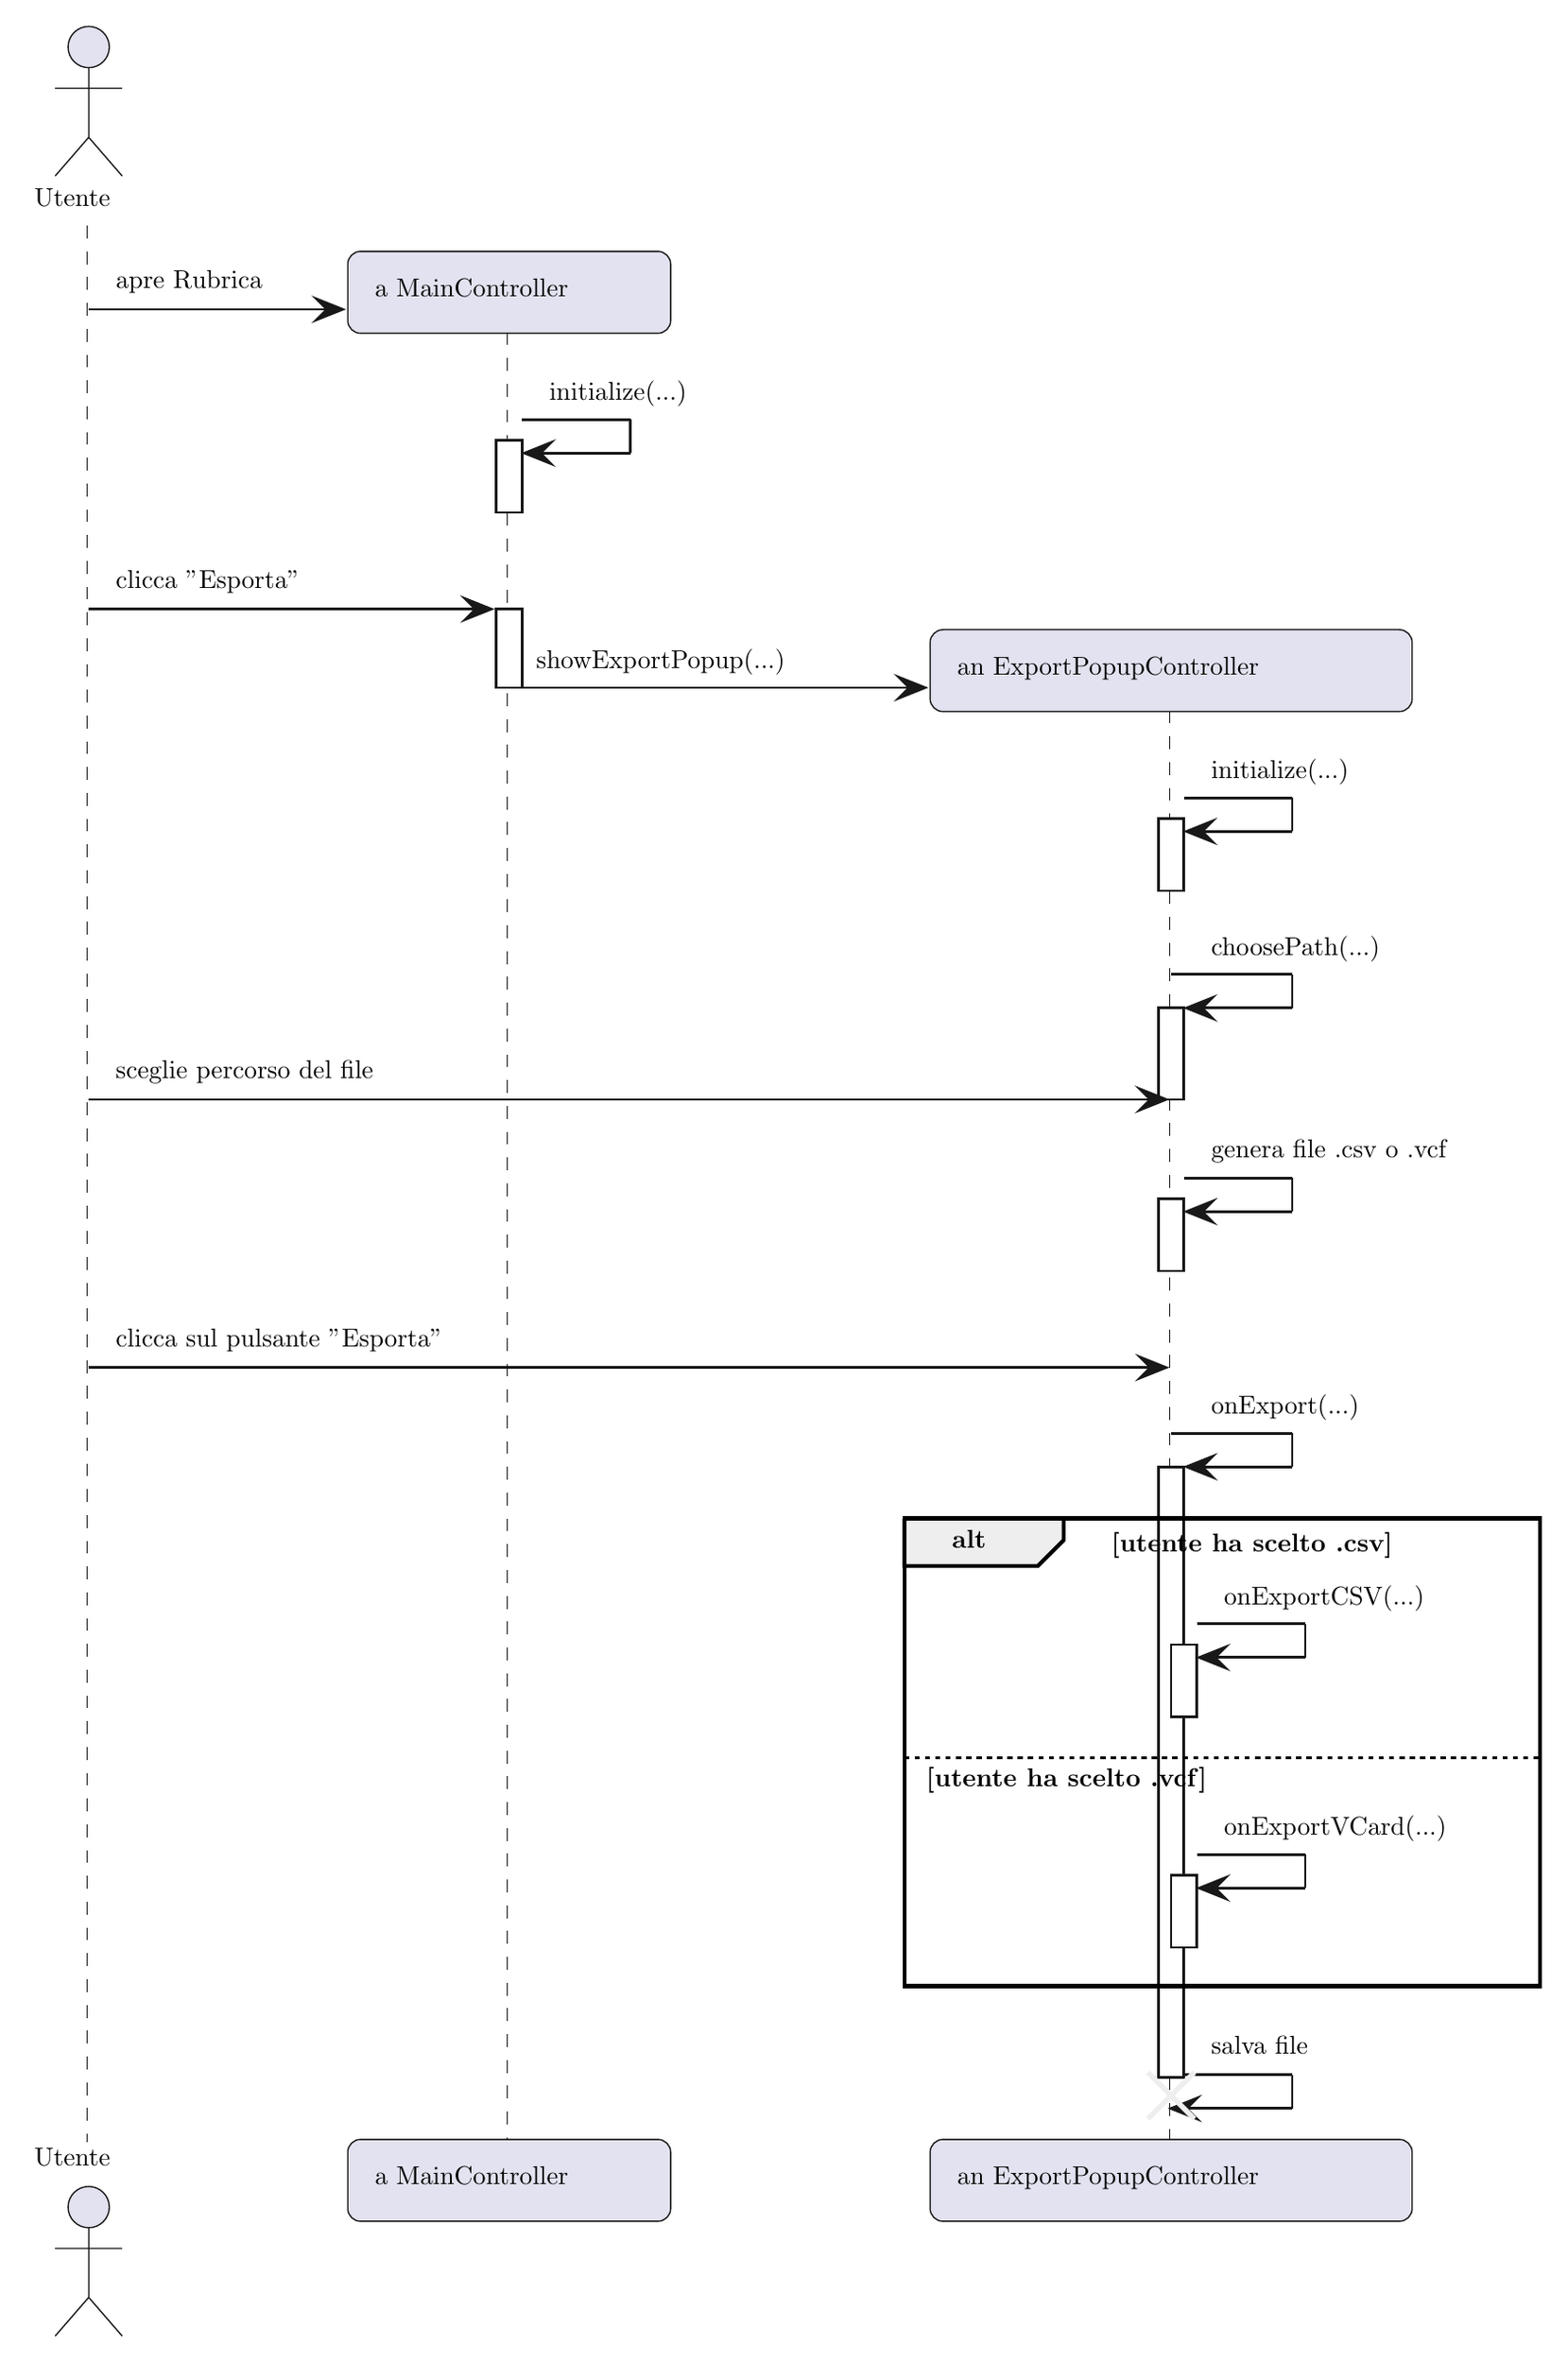
\begin{tikzpicture}[yscale=-1
,pstyle0/.style={color=plantucolor0001,fill=white,line width=1.0pt}
,pstyle1/.style={color=black,line width=1.5pt}
,pstyle2/.style={color=plantucolor0001,line width=0.5pt,dash pattern=on 5.0pt off 5.0pt}
,pstyle3/.style={color=plantucolor0001,fill=plantucolor0003,line width=0.5pt}
,pstyle4/.style={color=plantucolor0001,line width=0.5pt}
,pstyle5/.style={color=plantucolor0001,fill=plantucolor0001,line width=1.0pt}
,pstyle6/.style={color=plantucolor0001,line width=1.0pt}
,pstyle9/.style={color=plantucolor0005,line width=2.0pt}
]
\draw[pstyle0] (187.6937pt,165.9707pt) rectangle (197.6937pt,193.9707pt);
\draw[pstyle0] (187.6937pt,231.4492pt) rectangle (197.6937pt,261.9277pt);
\draw[pstyle0] (444.4229pt,312.6738pt) rectangle (454.4229pt,340.6738pt);
\draw[pstyle0] (444.4229pt,386.1523pt) rectangle (454.4229pt,421.6309pt);
\draw[pstyle0] (444.4229pt,460.1094pt) rectangle (454.4229pt,488.1094pt);
\draw[pstyle0] (444.4229pt,564.0664pt) rectangle (454.4229pt,800.9238pt);
\draw[pstyle0] (449.4229pt,633.0234pt) rectangle (459.4229pt,661.0234pt);
\draw[pstyle0] (449.4229pt,722.4453pt) rectangle (459.4229pt,750.4453pt);
\draw[pstyle1] (345.9372pt,584.0664pt) rectangle (592.5535pt,765.4453pt);
\draw[pstyle2] (29pt,82.7461pt) -- (29pt,825.9238pt);
\draw[pstyle2] (192.0597pt,124.1191pt) -- (192.0597pt,825.9238pt);
\draw[pstyle2] (448.9372pt,270.8223pt) -- (448.9372pt,825.9238pt);
\node at (5pt,65pt)[below right,color=black]{Utente};
\draw[pstyle3] (29.6pt,13.5pt) ellipse (8pt and 8pt);
\draw[pstyle4] (29.6pt,21.5pt) -- (29.6pt,48.5pt)(16.6pt,29.5pt) -- (42.6pt,29.5pt)(29.6pt,48.5pt) -- (16.6pt,63.5pt)(29.6pt,48.5pt) -- (42.6pt,63.5pt);
\node at (5pt,824.9238pt)[below right,color=black]{Utente};
\draw[pstyle3] (29.6pt,851.1699pt) ellipse (8pt and 8pt);
\draw[pstyle4] (29.6pt,859.1699pt) -- (29.6pt,886.1699pt)(16.6pt,867.1699pt) -- (42.6pt,867.1699pt)(29.6pt,886.1699pt) -- (16.6pt,901.1699pt)(29.6pt,886.1699pt) -- (42.6pt,901.1699pt);
\draw[pstyle3] (130.0597pt,829.9238pt) arc (180:270:5pt) -- (135.0597pt,824.9238pt) -- (250.3278pt,824.9238pt) arc (270:360:5pt) -- (255.3278pt,829.9238pt) -- (255.3278pt,851.6699pt) arc (0:90:5pt) -- (250.3278pt,856.6699pt) -- (135.0597pt,856.6699pt) arc (90:180:5pt) -- (130.0597pt,851.6699pt) -- cycle;
\node at (137.0597pt,831.9238pt)[below right,color=black]{a MainController};
\draw[pstyle3] (355.9372pt,829.9238pt) arc (180:270:5pt) -- (360.9372pt,824.9238pt) -- (537.9087pt,824.9238pt) arc (270:360:5pt) -- (542.9087pt,829.9238pt) -- (542.9087pt,851.6699pt) arc (0:90:5pt) -- (537.9087pt,856.6699pt) -- (360.9372pt,856.6699pt) arc (90:180:5pt) -- (355.9372pt,851.6699pt) -- cycle;
\node at (362.9372pt,831.9238pt)[below right,color=black]{an ExportPopupController};
\draw[pstyle0] (187.6937pt,165.9707pt) rectangle (197.6937pt,193.9707pt);
\draw[pstyle0] (187.6937pt,231.4492pt) rectangle (197.6937pt,261.9277pt);
\draw[pstyle0] (444.4229pt,312.6738pt) rectangle (454.4229pt,340.6738pt);
\draw[pstyle0] (444.4229pt,386.1523pt) rectangle (454.4229pt,421.6309pt);
\draw[pstyle0] (444.4229pt,460.1094pt) rectangle (454.4229pt,488.1094pt);
\draw[pstyle0] (444.4229pt,564.0664pt) rectangle (454.4229pt,800.9238pt);
\draw[pstyle0] (449.4229pt,633.0234pt) rectangle (459.4229pt,661.0234pt);
\draw[pstyle0] (449.4229pt,722.4453pt) rectangle (459.4229pt,750.4453pt);
\draw[pstyle5] (118.0597pt,111.2246pt) -- (128.0597pt,115.2246pt) -- (118.0597pt,119.2246pt) -- (122.0597pt,115.2246pt) -- cycle;
\draw[pstyle6] (29.6pt,115.2246pt) -- (124.0597pt,115.2246pt);
\node at (36.6pt,96.7461pt)[below right,color=black]{apre Rubrica};
\draw[pstyle3] (130.0597pt,97.7461pt) arc (180:270:5pt) -- (135.0597pt,92.7461pt) -- (250.3278pt,92.7461pt) arc (270:360:5pt) -- (255.3278pt,97.7461pt) -- (255.3278pt,119.4922pt) arc (0:90:5pt) -- (250.3278pt,124.4922pt) -- (135.0597pt,124.4922pt) arc (90:180:5pt) -- (130.0597pt,119.4922pt) -- cycle;
\node at (137.0597pt,99.7461pt)[below right,color=black]{a MainController};
\draw[pstyle6] (197.6937pt,157.9707pt) -- (239.6937pt,157.9707pt);
\draw[pstyle6] (239.6937pt,157.9707pt) -- (239.6937pt,170.9707pt);
\draw[pstyle6] (198.6937pt,170.9707pt) -- (239.6937pt,170.9707pt);
\draw[pstyle5] (208.6937pt,166.9707pt) -- (198.6937pt,170.9707pt) -- (208.6937pt,174.9707pt) -- (204.6937pt,170.9707pt) -- cycle;
\node at (204.6937pt,139.4922pt)[below right,color=black]{initialize(...)};
\draw[pstyle5] (175.6937pt,227.4492pt) -- (185.6937pt,231.4492pt) -- (175.6937pt,235.4492pt) -- (179.6937pt,231.4492pt) -- cycle;
\draw[pstyle6] (29.6pt,231.4492pt) -- (181.6937pt,231.4492pt);
\node at (36.6pt,212.9707pt)[below right,color=black]{clicca "Esporta"};
\draw[pstyle5] (343.9372pt,257.9277pt) -- (353.9372pt,261.9277pt) -- (343.9372pt,265.9277pt) -- (347.9372pt,261.9277pt) -- cycle;
\draw[pstyle6] (192.6937pt,261.9277pt) -- (349.9372pt,261.9277pt);
\node at (199.6937pt,243.4492pt)[below right,color=black]{showExportPopup(...)};
\draw[pstyle3] (355.9372pt,244.4492pt) arc (180:270:5pt) -- (360.9372pt,239.4492pt) -- (537.9087pt,239.4492pt) arc (270:360:5pt) -- (542.9087pt,244.4492pt) -- (542.9087pt,266.1953pt) arc (0:90:5pt) -- (537.9087pt,271.1953pt) -- (360.9372pt,271.1953pt) arc (90:180:5pt) -- (355.9372pt,266.1953pt) -- cycle;
\node at (362.9372pt,246.4492pt)[below right,color=black]{an ExportPopupController};
\draw[pstyle6] (454.4229pt,304.6738pt) -- (496.4229pt,304.6738pt);
\draw[pstyle6] (496.4229pt,304.6738pt) -- (496.4229pt,317.6738pt);
\draw[pstyle6] (455.4229pt,317.6738pt) -- (496.4229pt,317.6738pt);
\draw[pstyle5] (465.4229pt,313.6738pt) -- (455.4229pt,317.6738pt) -- (465.4229pt,321.6738pt) -- (461.4229pt,317.6738pt) -- cycle;
\node at (461.4229pt,286.1953pt)[below right,color=black]{initialize(...)};
\draw[pstyle6] (449.4229pt,373.1523pt) -- (496.4229pt,373.1523pt);
\draw[pstyle6] (496.4229pt,373.1523pt) -- (496.4229pt,386.1523pt);
\draw[pstyle6] (455.4229pt,386.1523pt) -- (496.4229pt,386.1523pt);
\draw[pstyle5] (465.4229pt,382.1523pt) -- (455.4229pt,386.1523pt) -- (465.4229pt,390.1523pt) -- (461.4229pt,386.1523pt) -- cycle;
\node at (461.4229pt,354.6738pt)[below right,color=black]{choosePath(...)};
\draw[pstyle5] (437.4229pt,417.6309pt) -- (447.4229pt,421.6309pt) -- (437.4229pt,425.6309pt) -- (441.4229pt,421.6309pt) -- cycle;
\draw[pstyle6] (29.6pt,421.6309pt) -- (443.4229pt,421.6309pt);
\node at (36.6pt,403.1523pt)[below right,color=black]{sceglie percorso del file};
\draw[pstyle6] (454.4229pt,452.1094pt) -- (496.4229pt,452.1094pt);
\draw[pstyle6] (496.4229pt,452.1094pt) -- (496.4229pt,465.1094pt);
\draw[pstyle6] (455.4229pt,465.1094pt) -- (496.4229pt,465.1094pt);
\draw[pstyle5] (465.4229pt,461.1094pt) -- (455.4229pt,465.1094pt) -- (465.4229pt,469.1094pt) -- (461.4229pt,465.1094pt) -- cycle;
\node at (461.4229pt,433.6309pt)[below right,color=black]{genera file .csv o .vcf};
\draw[pstyle5] (437.4229pt,521.5879pt) -- (447.4229pt,525.5879pt) -- (437.4229pt,529.5879pt) -- (441.4229pt,525.5879pt) -- cycle;
\draw[pstyle6] (29.6pt,525.5879pt) -- (443.4229pt,525.5879pt);
\node at (36.6pt,507.1094pt)[below right,color=black]{clicca sul pulsante "Esporta"};
\draw[pstyle6] (449.4229pt,551.0664pt) -- (496.4229pt,551.0664pt);
\draw[pstyle6] (496.4229pt,551.0664pt) -- (496.4229pt,564.0664pt);
\draw[pstyle6] (455.4229pt,564.0664pt) -- (496.4229pt,564.0664pt);
\draw[pstyle5] (465.4229pt,560.0664pt) -- (455.4229pt,564.0664pt) -- (465.4229pt,568.0664pt) -- (461.4229pt,564.0664pt) -- cycle;
\node at (461.4229pt,532.5879pt)[below right,color=black]{onExport(...)};
\draw[color=black,fill=plantucolor0004,line width=1.5pt] (345.9372pt,584.0664pt) -- (407.7372pt,584.0664pt) -- (407.7372pt,592.5449pt) -- (397.7372pt,602.5449pt) -- (345.9372pt,602.5449pt) -- (345.9372pt,584.0664pt);
\draw[pstyle1] (345.9372pt,584.0664pt) rectangle (592.5535pt,765.4453pt);
\node at (360.9372pt,585.0664pt)[below right,color=black]{\textbf{alt}};
\node at (422.7372pt,586.0664pt)[below right,color=black]{\textbf{[utente ha scelto .csv]}};
\draw[pstyle6] (459.4229pt,625.0234pt) -- (501.4229pt,625.0234pt);
\draw[pstyle6] (501.4229pt,625.0234pt) -- (501.4229pt,638.0234pt);
\draw[pstyle6] (460.4229pt,638.0234pt) -- (501.4229pt,638.0234pt);
\draw[pstyle5] (470.4229pt,634.0234pt) -- (460.4229pt,638.0234pt) -- (470.4229pt,642.0234pt) -- (466.4229pt,638.0234pt) -- cycle;
\node at (466.4229pt,606.5449pt)[below right,color=black]{onExportCSV(...)};
\draw[color=black,line width=1.0pt,dash pattern=on 2.0pt off 2.0pt] (345.9372pt,677.0234pt) -- (592.5535pt,677.0234pt);
\node at (350.9372pt,677.0234pt)[below right,color=black]{\textbf{[utente ha scelto .vcf]}};
\draw[pstyle6] (459.4229pt,714.4453pt) -- (501.4229pt,714.4453pt);
\draw[pstyle6] (501.4229pt,714.4453pt) -- (501.4229pt,727.4453pt);
\draw[pstyle6] (460.4229pt,727.4453pt) -- (501.4229pt,727.4453pt);
\draw[pstyle5] (470.4229pt,723.4453pt) -- (460.4229pt,727.4453pt) -- (470.4229pt,731.4453pt) -- (466.4229pt,727.4453pt) -- cycle;
\node at (466.4229pt,695.9668pt)[below right,color=black]{onExportVCard(...)};
\draw[pstyle6] (454.4229pt,799.9238pt) -- (496.4229pt,799.9238pt);
\draw[pstyle6] (496.4229pt,799.9238pt) -- (496.4229pt,812.9238pt);
\draw[pstyle6] (449.4229pt,812.9238pt) -- (496.4229pt,812.9238pt);
\draw[pstyle5] (459.4229pt,808.9238pt) -- (449.4229pt,812.9238pt) -- (459.4229pt,816.9238pt) -- (455.4229pt,812.9238pt) -- cycle;
\node at (461.4229pt,781.4453pt)[below right,color=black]{salva file};
\draw[pstyle9] (440.4229pt,798.9238pt) -- (458.4229pt,816.9238pt);
\draw[pstyle9] (440.4229pt,816.9238pt) -- (458.4229pt,798.9238pt);
\end{tikzpicture}
}
\end{adjustbox}

\begin{figure}[h]
	\caption{Diagramma sequenza C6 - Esportare rubrica}
	\label{fig:Diagramma sequenza C6 - Esportare rubrica}
\end{figure}

\newpage
\subsubsection{C8 - Salvare rubrica}
Il seguente diagramma di sequenza illustra l'esecuzione del caso d'uso C8:
% generated by Plantuml 1.2024.3       
\definecolor{plantucolor0000}{RGB}{255,255,255}
\definecolor{plantucolor0001}{RGB}{24,24,24}
\definecolor{plantucolor0002}{RGB}{0,0,0}
\definecolor{plantucolor0003}{RGB}{226,226,240}
\definecolor{plantucolor0004}{RGB}{254,255,221}
\definecolor{plantucolor0005}{RGB}{238,238,238}

\begin{adjustbox}{width=.9\paperwidth, center}
	\resizebox{\textwidth}{!}{
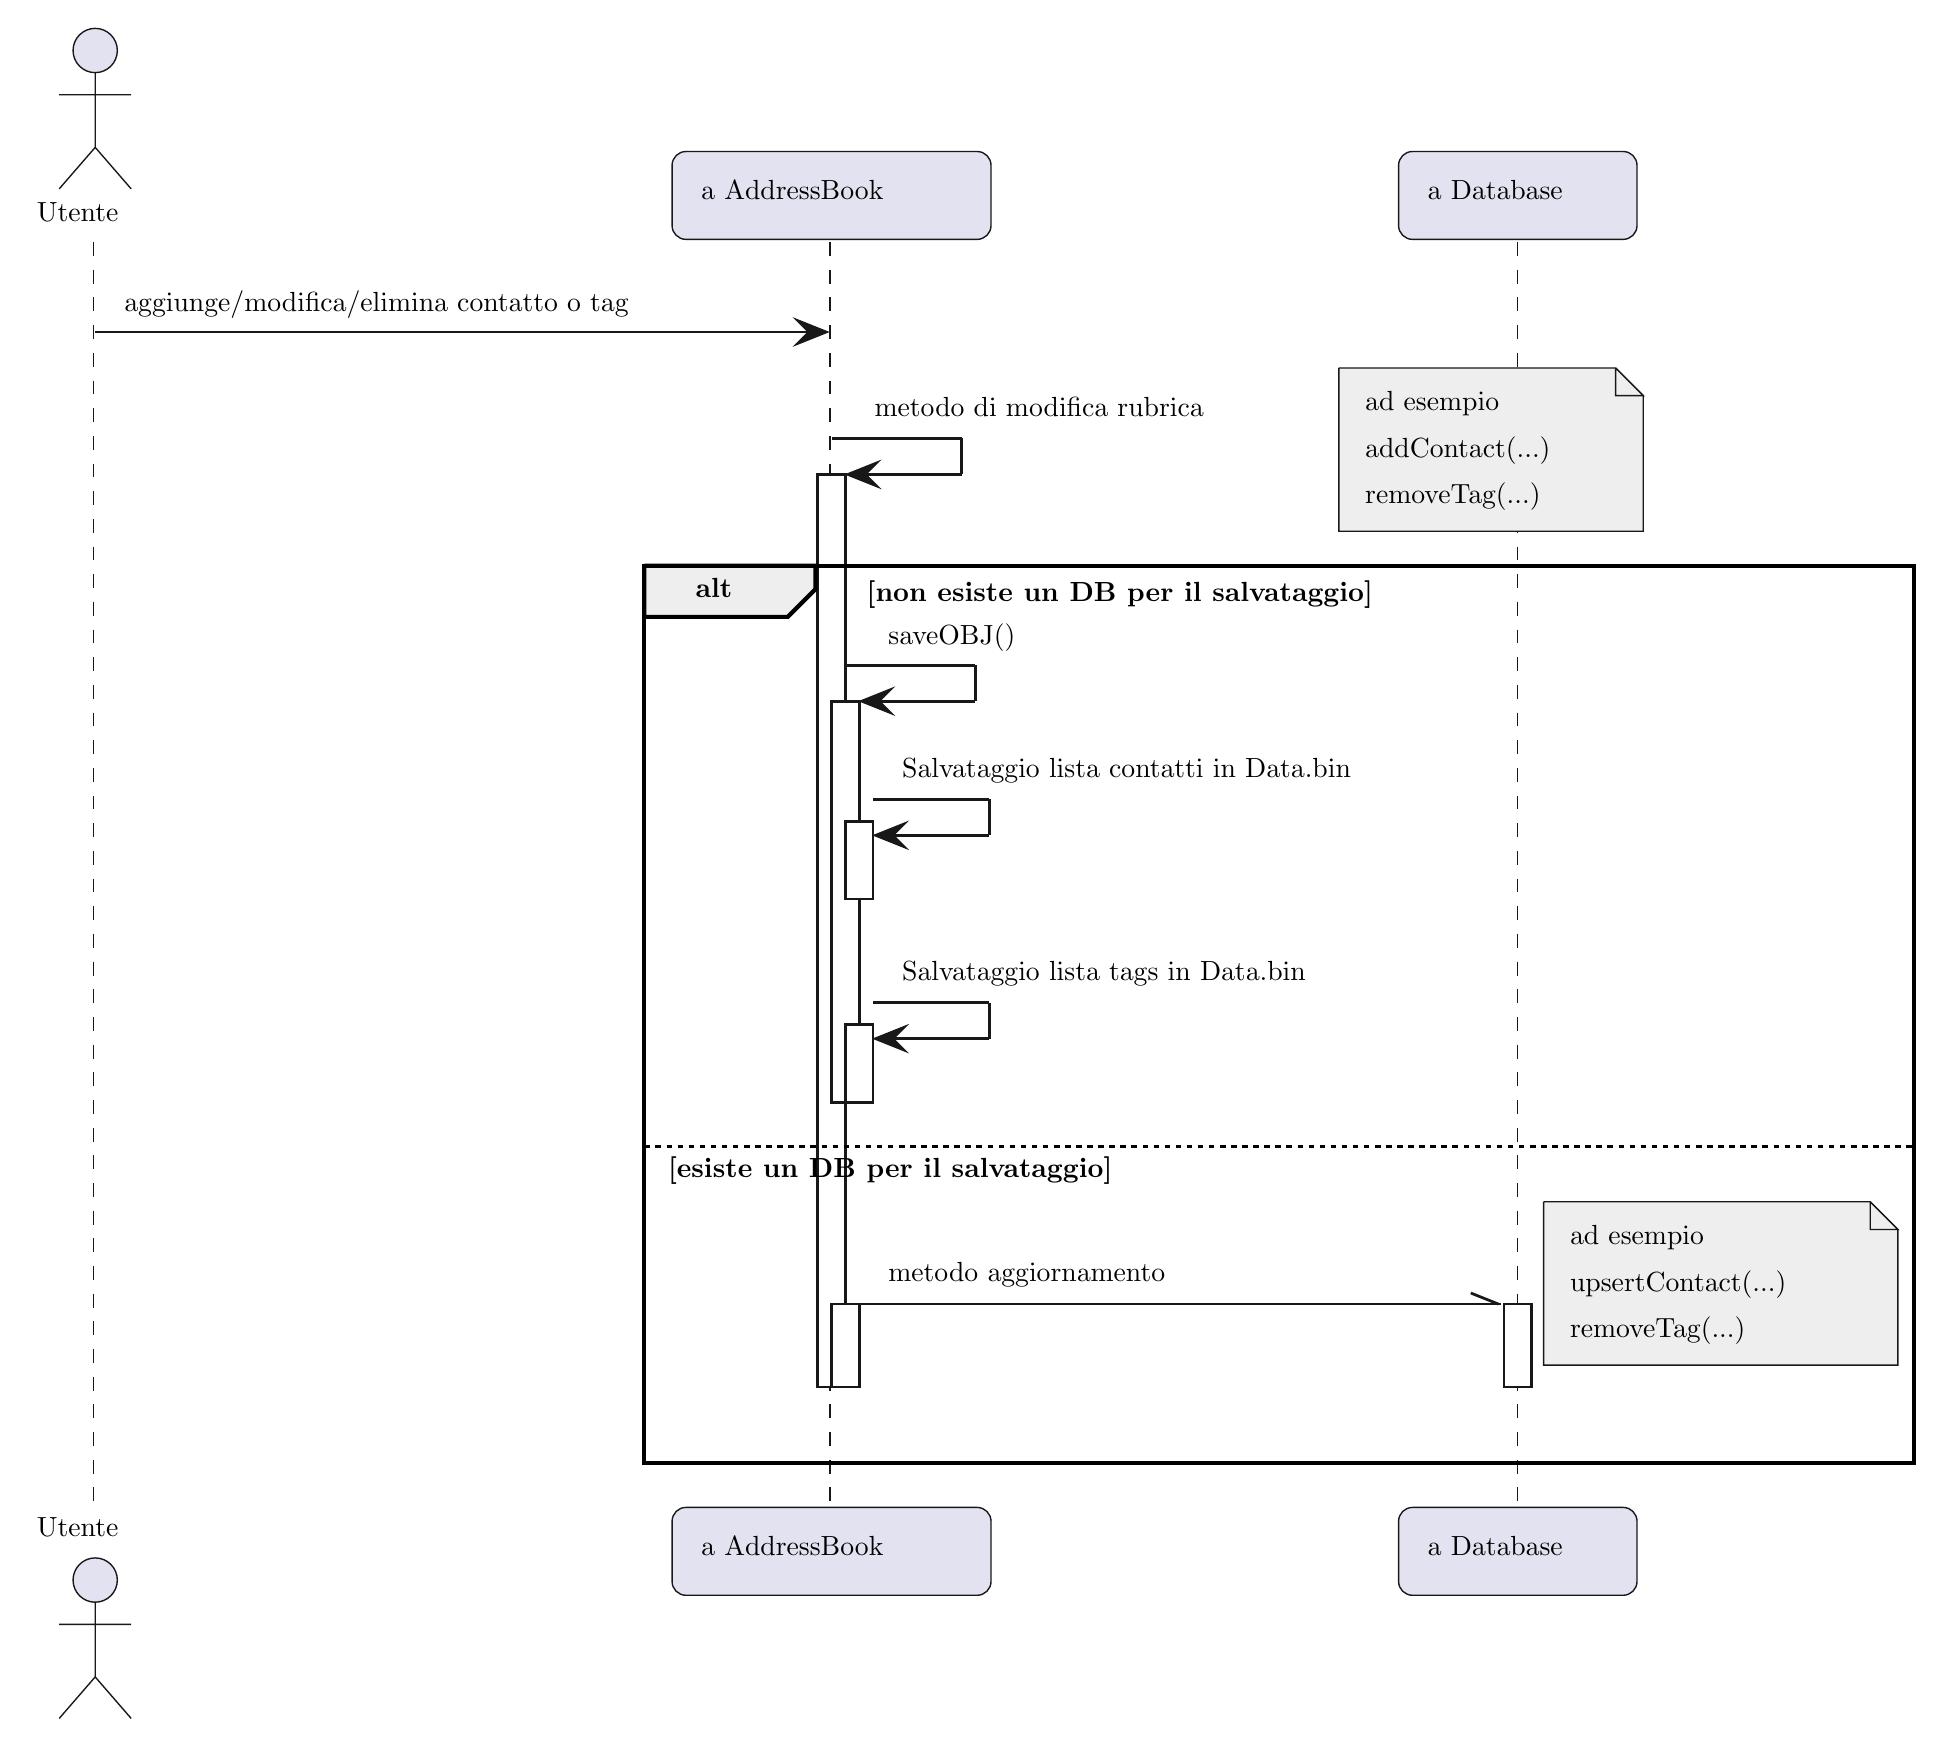
\begin{tikzpicture}[yscale=-1
,pstyle0/.style={color=plantucolor0001,fill=white,line width=1.0pt}
,pstyle1/.style={color=black,line width=1.5pt}
,pstyle2/.style={color=plantucolor0001,line width=0.5pt,dash pattern=on 5.0pt off 5.0pt}
,pstyle3/.style={color=plantucolor0001,fill=plantucolor0003,line width=0.5pt}
,pstyle4/.style={color=plantucolor0001,line width=0.5pt}
,pstyle5/.style={color=plantucolor0001,fill=plantucolor0001,line width=1.0pt}
,pstyle6/.style={color=plantucolor0001,line width=1.0pt}
,pstyle7/.style={color=plantucolor0001,fill=plantucolor0004,line width=0.5pt}
]
\draw[pstyle0] (290.6771pt,166.6816pt) rectangle (300.6771pt,496.4746pt);
\draw[pstyle0] (295.6771pt,248.6172pt) rectangle (305.6771pt,393.5742pt);
\draw[pstyle0] (300.6771pt,292.0957pt) rectangle (310.6771pt,320.0957pt);
\draw[pstyle0] (300.6771pt,365.5742pt) rectangle (310.6771pt,393.5742pt);
\draw[pstyle0] (295.6771pt,466.4746pt) rectangle (305.6771pt,496.4746pt);
\draw[pstyle0] (538.6553pt,466.4746pt) rectangle (548.6553pt,496.4746pt);
\draw[pstyle1] (228.0535pt,199.6602pt) rectangle (686.7392pt,523.9531pt);
\draw[pstyle2] (29pt,82.7461pt) -- (29pt,540.9531pt);
\draw[pstyle2] (295.0535pt,82.7461pt) -- (295.0535pt,540.9531pt);
\draw[pstyle2] (543.5799pt,82.7461pt) -- (543.5799pt,540.9531pt);
\node at (5pt,65pt)[below right,color=black]{Utente};
\draw[pstyle3] (29.6pt,13.5pt) ellipse (8pt and 8pt);
\draw[pstyle4] (29.6pt,21.5pt) -- (29.6pt,48.5pt)(16.6pt,29.5pt) -- (42.6pt,29.5pt)(29.6pt,48.5pt) -- (16.6pt,63.5pt)(29.6pt,48.5pt) -- (42.6pt,63.5pt);
\node at (5pt,539.9531pt)[below right,color=black]{Utente};
\draw[pstyle3] (29.6pt,566.1992pt) ellipse (8pt and 8pt);
\draw[pstyle4] (29.6pt,574.1992pt) -- (29.6pt,601.1992pt)(16.6pt,582.1992pt) -- (42.6pt,582.1992pt)(29.6pt,601.1992pt) -- (16.6pt,616.1992pt)(29.6pt,601.1992pt) -- (42.6pt,616.1992pt);
\draw[pstyle3] (238.0535pt,55pt) arc (180:270:5pt) -- (243.0535pt,50pt) -- (348.3006pt,50pt) arc (270:360:5pt) -- (353.3006pt,55pt) -- (353.3006pt,76.7461pt) arc (0:90:5pt) -- (348.3006pt,81.7461pt) -- (243.0535pt,81.7461pt) arc (90:180:5pt) -- (238.0535pt,76.7461pt) -- cycle;
\node at (245.0535pt,57pt)[below right,color=black]{a AddressBook};
\draw[pstyle3] (238.0535pt,544.9531pt) arc (180:270:5pt) -- (243.0535pt,539.9531pt) -- (348.3006pt,539.9531pt) arc (270:360:5pt) -- (353.3006pt,544.9531pt) -- (353.3006pt,566.6992pt) arc (0:90:5pt) -- (348.3006pt,571.6992pt) -- (243.0535pt,571.6992pt) arc (90:180:5pt) -- (238.0535pt,566.6992pt) -- cycle;
\node at (245.0535pt,546.9531pt)[below right,color=black]{a AddressBook};
\draw[pstyle3] (500.5799pt,55pt) arc (180:270:5pt) -- (505.5799pt,50pt) -- (581.7307pt,50pt) arc (270:360:5pt) -- (586.7307pt,55pt) -- (586.7307pt,76.7461pt) arc (0:90:5pt) -- (581.7307pt,81.7461pt) -- (505.5799pt,81.7461pt) arc (90:180:5pt) -- (500.5799pt,76.7461pt) -- cycle;
\node at (507.5799pt,57pt)[below right,color=black]{a Database};
\draw[pstyle3] (500.5799pt,544.9531pt) arc (180:270:5pt) -- (505.5799pt,539.9531pt) -- (581.7307pt,539.9531pt) arc (270:360:5pt) -- (586.7307pt,544.9531pt) -- (586.7307pt,566.6992pt) arc (0:90:5pt) -- (581.7307pt,571.6992pt) -- (505.5799pt,571.6992pt) arc (90:180:5pt) -- (500.5799pt,566.6992pt) -- cycle;
\node at (507.5799pt,546.9531pt)[below right,color=black]{a Database};
\draw[pstyle0] (290.6771pt,166.6816pt) rectangle (300.6771pt,496.4746pt);
\draw[pstyle0] (295.6771pt,248.6172pt) rectangle (305.6771pt,393.5742pt);
\draw[pstyle0] (300.6771pt,292.0957pt) rectangle (310.6771pt,320.0957pt);
\draw[pstyle0] (300.6771pt,365.5742pt) rectangle (310.6771pt,393.5742pt);
\draw[pstyle0] (295.6771pt,466.4746pt) rectangle (305.6771pt,496.4746pt);
\draw[pstyle0] (538.6553pt,466.4746pt) rectangle (548.6553pt,496.4746pt);
\draw[pstyle5] (283.6771pt,111.2246pt) -- (293.6771pt,115.2246pt) -- (283.6771pt,119.2246pt) -- (287.6771pt,115.2246pt) -- cycle;
\draw[pstyle6] (29.6pt,115.2246pt) -- (289.6771pt,115.2246pt);
\node at (36.6pt,96.7461pt)[below right,color=black]{aggiunge/modifica/elimina contatto o tag};
\draw[pstyle6] (295.6771pt,153.6816pt) -- (342.6771pt,153.6816pt);
\draw[pstyle6] (342.6771pt,153.6816pt) -- (342.6771pt,166.6816pt);
\draw[pstyle6] (301.6771pt,166.6816pt) -- (342.6771pt,166.6816pt);
\draw[pstyle5] (311.6771pt,162.6816pt) -- (301.6771pt,166.6816pt) -- (311.6771pt,170.6816pt) -- (307.6771pt,166.6816pt) -- cycle;
\node at (307.6771pt,135.2031pt)[below right,color=black]{metodo di modifica rubrica};
\draw[pstyle7] (478.9801pt,128.2246pt) -- (478.9801pt,187.2246pt) -- (588.9801pt,187.2246pt) -- (588.9801pt,138.2246pt) -- (578.9801pt,128.2246pt) -- (478.9801pt,128.2246pt);
\draw[pstyle7] (578.9801pt,128.2246pt) -- (578.9801pt,138.2246pt) -- (588.9801pt,138.2246pt) -- (578.9801pt,128.2246pt);
\node at (484.9801pt,133.2246pt)[below right,color=black]{ad esempio};
\node at (484.9801pt,149.7031pt)[below right,color=black]{addContact(...)};
\node at (484.9801pt,166.1816pt)[below right,color=black]{removeTag(...)};
\draw[color=black,fill=plantucolor0005,line width=1.5pt] (228.0535pt,199.6602pt) -- (289.8535pt,199.6602pt) -- (289.8535pt,208.1387pt) -- (279.8535pt,218.1387pt) -- (228.0535pt,218.1387pt) -- (228.0535pt,199.6602pt);
\draw[pstyle1] (228.0535pt,199.6602pt) rectangle (686.7392pt,523.9531pt);
\node at (243.0535pt,200.6602pt)[below right,color=black]{\textbf{alt}};
\node at (304.8535pt,201.6602pt)[below right,color=black]{\textbf{[non esiste un DB per il salvataggio]}};
\draw[pstyle6] (300.6771pt,235.6172pt) -- (347.6771pt,235.6172pt);
\draw[pstyle6] (347.6771pt,235.6172pt) -- (347.6771pt,248.6172pt);
\draw[pstyle6] (306.6771pt,248.6172pt) -- (347.6771pt,248.6172pt);
\draw[pstyle5] (316.6771pt,244.6172pt) -- (306.6771pt,248.6172pt) -- (316.6771pt,252.6172pt) -- (312.6771pt,248.6172pt) -- cycle;
\node at (312.6771pt,217.1387pt)[below right,color=black]{saveOBJ()};
\draw[pstyle6] (310.6771pt,284.0957pt) -- (352.6771pt,284.0957pt);
\draw[pstyle6] (352.6771pt,284.0957pt) -- (352.6771pt,297.0957pt);
\draw[pstyle6] (311.6771pt,297.0957pt) -- (352.6771pt,297.0957pt);
\draw[pstyle5] (321.6771pt,293.0957pt) -- (311.6771pt,297.0957pt) -- (321.6771pt,301.0957pt) -- (317.6771pt,297.0957pt) -- cycle;
\node at (317.6771pt,265.6172pt)[below right,color=black]{Salvataggio lista contatti in Data.bin};
\draw[pstyle6] (310.6771pt,357.5742pt) -- (352.6771pt,357.5742pt);
\draw[pstyle6] (352.6771pt,357.5742pt) -- (352.6771pt,370.5742pt);
\draw[pstyle6] (311.6771pt,370.5742pt) -- (352.6771pt,370.5742pt);
\draw[pstyle5] (321.6771pt,366.5742pt) -- (311.6771pt,370.5742pt) -- (321.6771pt,374.5742pt) -- (317.6771pt,370.5742pt) -- cycle;
\node at (317.6771pt,339.0957pt)[below right,color=black]{Salvataggio lista tags in Data.bin};
\draw[color=black,line width=1.0pt,dash pattern=on 2.0pt off 2.0pt] (228.0535pt,409.5742pt) -- (686.7392pt,409.5742pt);
\node at (233.0535pt,409.5742pt)[below right,color=black]{\textbf{[esiste un DB per il salvataggio]}};
\draw[pstyle6] (536.6553pt,466.4746pt) -- (526.6553pt,462.4746pt);
\draw[pstyle6] (305.6771pt,466.4746pt) -- (537.6553pt,466.4746pt);
\node at (312.6771pt,447.9961pt)[below right,color=black]{metodo aggiornamento};
\draw[pstyle7] (553pt,429.5176pt) -- (553pt,488.5176pt) -- (681pt,488.5176pt) -- (681pt,439.5176pt) -- (671pt,429.5176pt) -- (553pt,429.5176pt);
\draw[pstyle7] (671pt,429.5176pt) -- (671pt,439.5176pt) -- (681pt,439.5176pt) -- (671pt,429.5176pt);
\node at (559pt,434.5176pt)[below right,color=black]{ad esempio};
\node at (559pt,450.9961pt)[below right,color=black]{upsertContact(...)};
\node at (559pt,467.4746pt)[below right,color=black]{removeTag(...)};
\end{tikzpicture}
}
\end{adjustbox}

\begin{figure}[h]
	\caption{Diagramma sequenza C8 - Salvare rubrica}
	\label{fig:Diagramma sequenza C8 - Salvare rubrica}
\end{figure}

\newpage
\subsubsection{Aggiunta DB}
Il seguente diagramma di sequenza illustra il flusso di operazioni attraverso cui l'utente aggiunge un link a un Database, consentendo il salvataggio dei dati nel DB anziché in locale.:
% generated by Plantuml 1.2024.3       
\definecolor{plantucolor0000}{RGB}{255,255,255}
\definecolor{plantucolor0001}{RGB}{24,24,24}
\definecolor{plantucolor0002}{RGB}{0,0,0}
\definecolor{plantucolor0003}{RGB}{226,226,240}
\definecolor{plantucolor0004}{RGB}{254,255,221}
\definecolor{plantucolor0005}{RGB}{238,238,238}
\definecolor{plantucolor0006}{RGB}{168,0,54}

\begin{adjustbox}{width=.9\paperwidth, center}
	\resizebox{\textwidth}{!}{
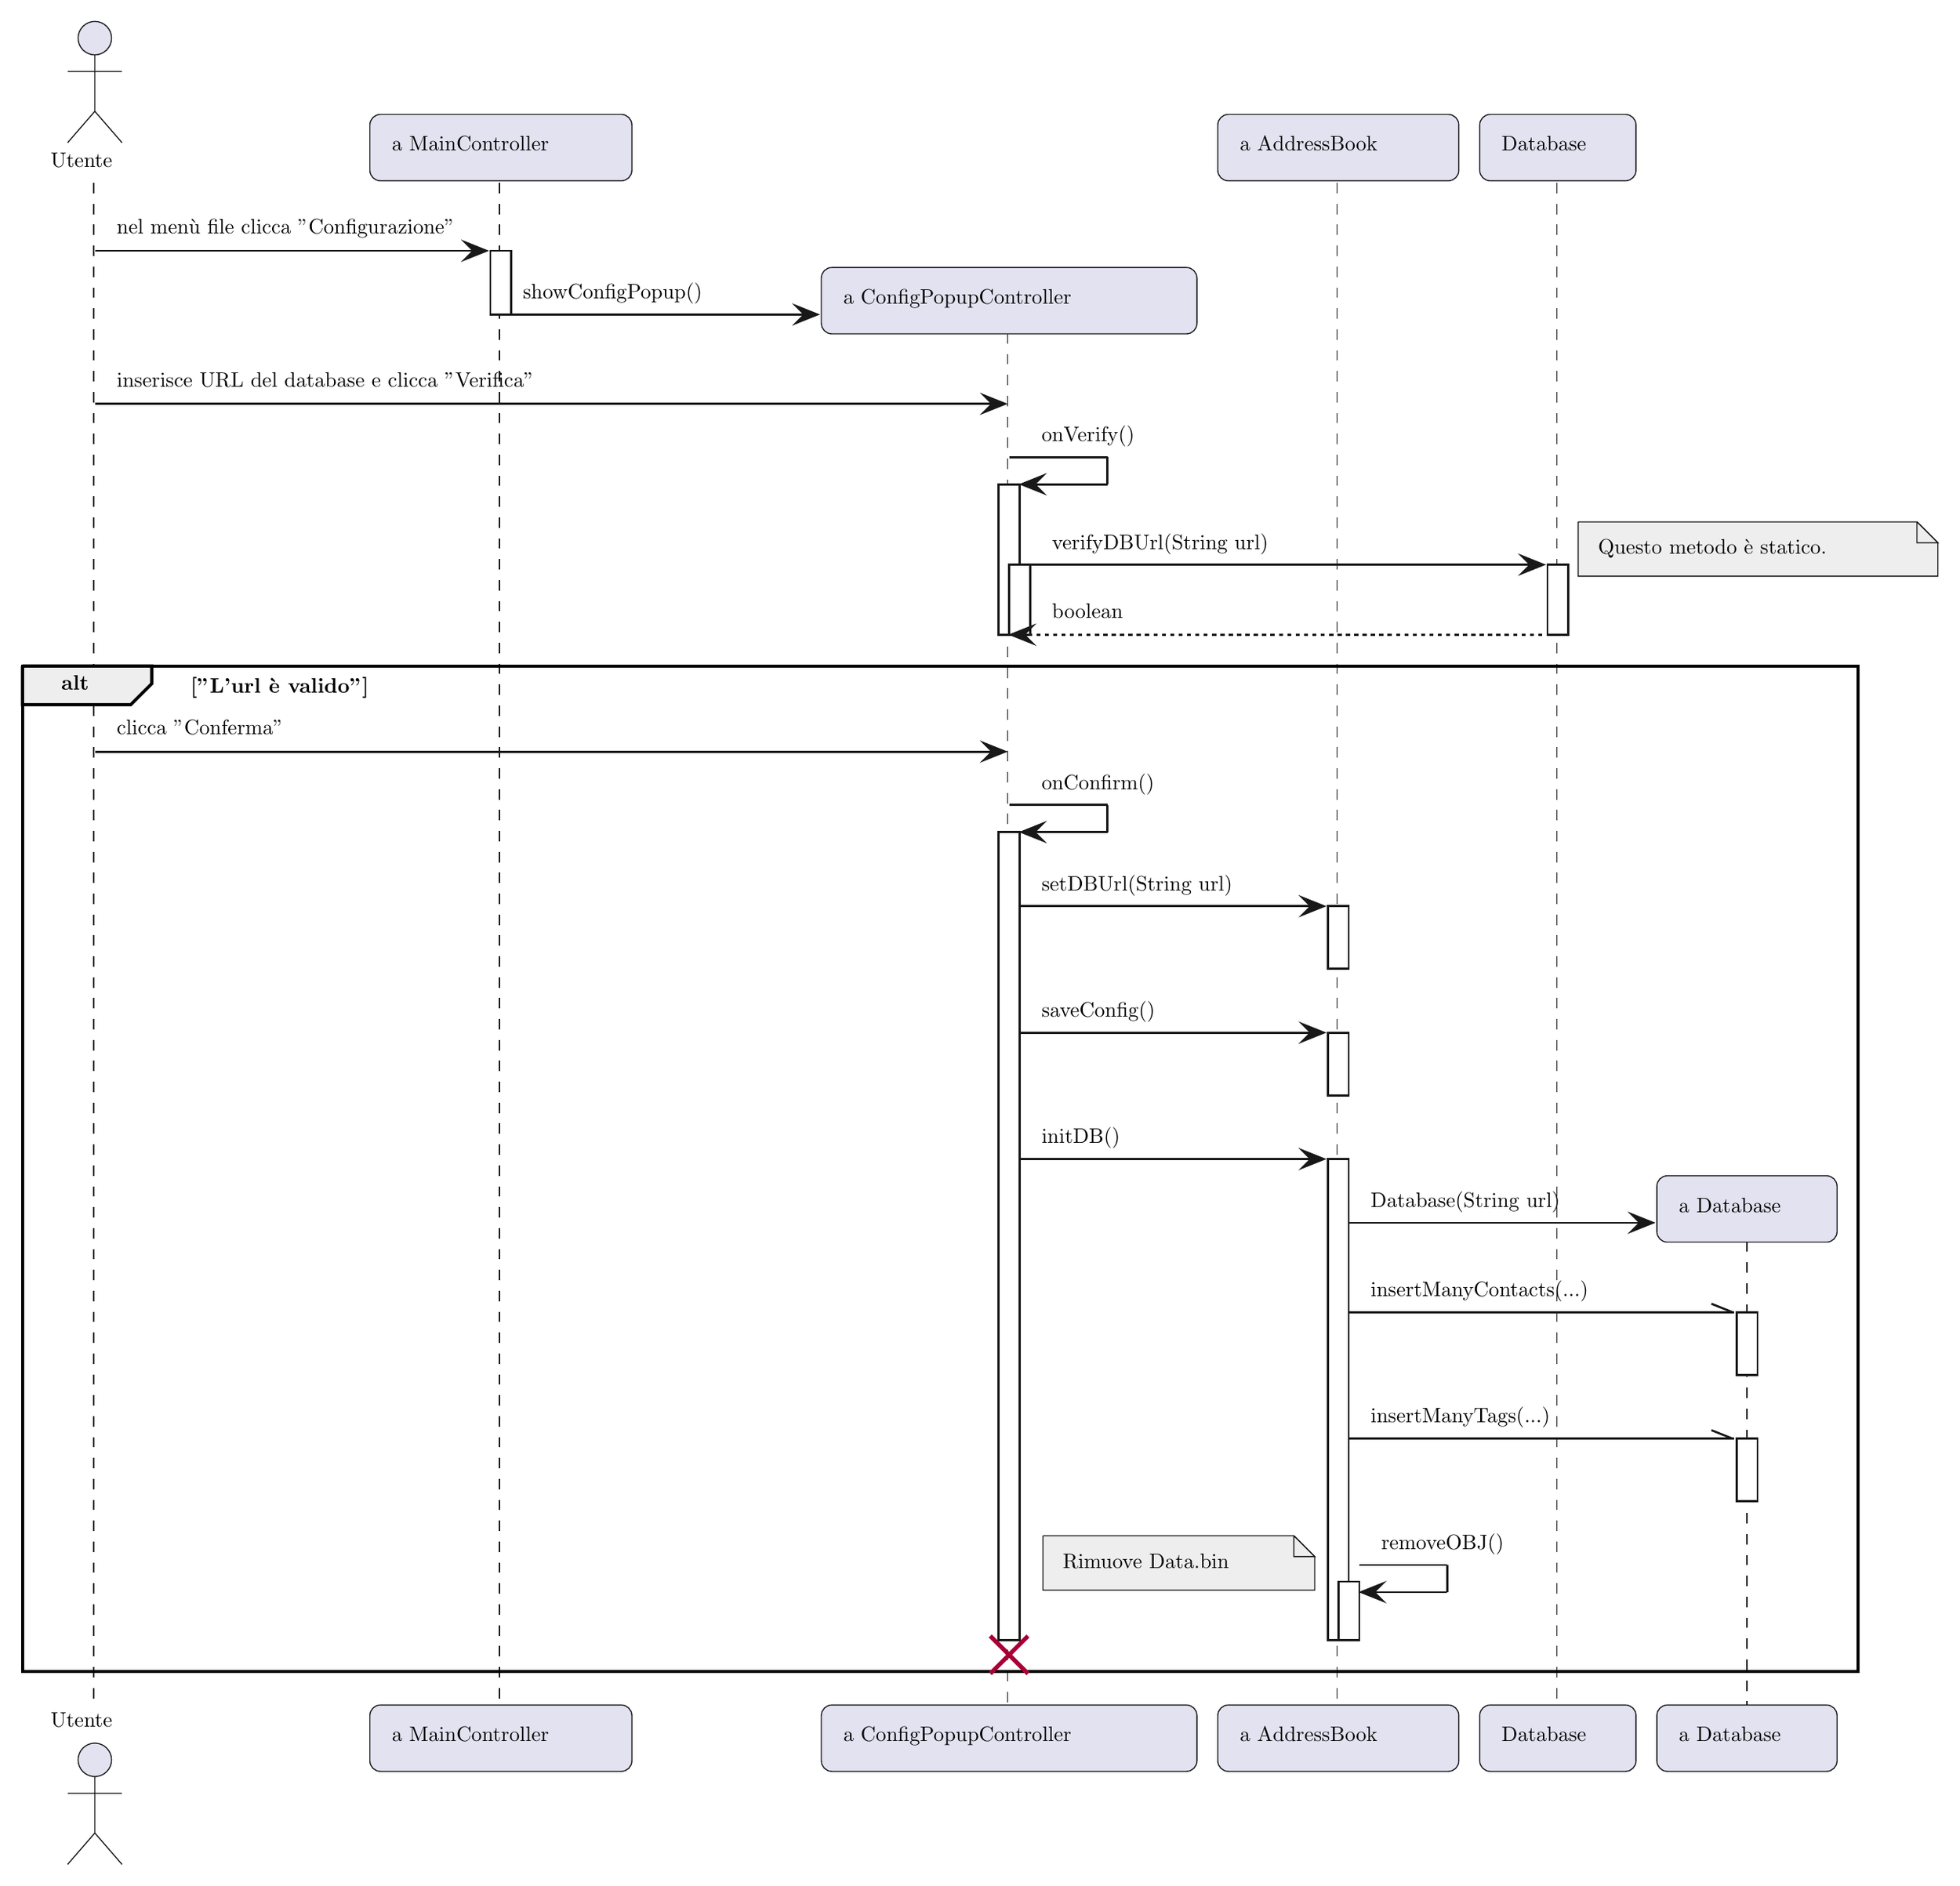
\begin{tikzpicture}[yscale=-1
,pstyle0/.style={color=plantucolor0001,fill=white,line width=1.0pt}
,pstyle1/.style={color=black,line width=1.5pt}
,pstyle2/.style={color=plantucolor0001,line width=0.5pt,dash pattern=on 5.0pt off 5.0pt}
,pstyle3/.style={color=plantucolor0001,fill=plantucolor0003,line width=0.5pt}
,pstyle4/.style={color=plantucolor0001,line width=0.5pt}
,pstyle5/.style={color=plantucolor0001,fill=plantucolor0001,line width=1.0pt}
,pstyle6/.style={color=plantucolor0001,line width=1.0pt}
,pstyle7/.style={color=plantucolor0001,fill=plantucolor0004,line width=0.5pt}
,pstyle10/.style={color=plantucolor0006,line width=2.0pt}
]
\draw[pstyle0] (233.7801pt,115.2246pt) rectangle (243.7801pt,145.7031pt);
\draw[pstyle0] (476.8468pt,226.9277pt) rectangle (486.8468pt,298.8848pt);
\draw[pstyle0] (481.8468pt,265.4063pt) rectangle (491.8468pt,298.8848pt);
\draw[pstyle0] (476.8468pt,393.3203pt) rectangle (486.8468pt,779.9375pt);
\draw[pstyle0] (634.2703pt,428.7988pt) rectangle (644.2703pt,458.7988pt);
\draw[pstyle0] (634.2703pt,489.2773pt) rectangle (644.2703pt,519.2773pt);
\draw[pstyle0] (634.2703pt,549.7559pt) rectangle (644.2703pt,779.9375pt);
\draw[pstyle0] (639.2703pt,751.9375pt) rectangle (649.2703pt,779.9375pt);
\draw[pstyle0] (739.2586pt,265.4063pt) rectangle (749.2586pt,298.8848pt);
\draw[pstyle0] (829.6987pt,622.9805pt) rectangle (839.6987pt,652.9805pt);
\draw[pstyle0] (829.6987pt,683.459pt) rectangle (839.6987pt,713.459pt);
\draw[pstyle1] (10pt,313.8848pt) rectangle (887.7741pt,794.9375pt);
\draw[pstyle2] (44pt,82.7461pt) -- (44pt,811.9375pt);
\draw[pstyle2] (238.1461pt,82.7461pt) -- (238.1461pt,811.9375pt);
\draw[pstyle2] (481.0468pt,154.5977pt) -- (481.0468pt,811.9375pt);
\draw[pstyle2] (638.6468pt,82.7461pt) -- (638.6468pt,811.9375pt);
\draw[pstyle2] (743.8939pt,82.7461pt) -- (743.8939pt,811.9375pt);
\draw[pstyle2] (834.6233pt,589.1289pt) -- (834.6233pt,811.9375pt);
\node at (20pt,65pt)[below right,color=black]{Utente};
\draw[pstyle3] (44.6pt,13.5pt) ellipse (8pt and 8pt);
\draw[pstyle4] (44.6pt,21.5pt) -- (44.6pt,48.5pt)(31.6pt,29.5pt) -- (57.6pt,29.5pt)(44.6pt,48.5pt) -- (31.6pt,63.5pt)(44.6pt,48.5pt) -- (57.6pt,63.5pt);
\node at (20pt,810.9375pt)[below right,color=black]{Utente};
\draw[pstyle3] (44.6pt,837.1836pt) ellipse (8pt and 8pt);
\draw[pstyle4] (44.6pt,845.1836pt) -- (44.6pt,872.1836pt)(31.6pt,853.1836pt) -- (57.6pt,853.1836pt)(44.6pt,872.1836pt) -- (31.6pt,887.1836pt)(44.6pt,872.1836pt) -- (57.6pt,887.1836pt);
\draw[pstyle3] (176.1461pt,55pt) arc (180:270:5pt) -- (181.1461pt,50pt) -- (296.4142pt,50pt) arc (270:360:5pt) -- (301.4142pt,55pt) -- (301.4142pt,76.7461pt) arc (0:90:5pt) -- (296.4142pt,81.7461pt) -- (181.1461pt,81.7461pt) arc (90:180:5pt) -- (176.1461pt,76.7461pt) -- cycle;
\node at (183.1461pt,57pt)[below right,color=black]{a MainController};
\draw[pstyle3] (176.1461pt,815.9375pt) arc (180:270:5pt) -- (181.1461pt,810.9375pt) -- (296.4142pt,810.9375pt) arc (270:360:5pt) -- (301.4142pt,815.9375pt) -- (301.4142pt,837.6836pt) arc (0:90:5pt) -- (296.4142pt,842.6836pt) -- (181.1461pt,842.6836pt) arc (90:180:5pt) -- (176.1461pt,837.6836pt) -- cycle;
\node at (183.1461pt,817.9375pt)[below right,color=black]{a MainController};
\draw[pstyle3] (392.0468pt,815.9375pt) arc (180:270:5pt) -- (397.0468pt,810.9375pt) -- (566.6468pt,810.9375pt) arc (270:360:5pt) -- (571.6468pt,815.9375pt) -- (571.6468pt,837.6836pt) arc (0:90:5pt) -- (566.6468pt,842.6836pt) -- (397.0468pt,842.6836pt) arc (90:180:5pt) -- (392.0468pt,837.6836pt) -- cycle;
\node at (399.0468pt,817.9375pt)[below right,color=black]{a ConfigPopupController};
\draw[pstyle3] (581.6468pt,55pt) arc (180:270:5pt) -- (586.6468pt,50pt) -- (691.8939pt,50pt) arc (270:360:5pt) -- (696.8939pt,55pt) -- (696.8939pt,76.7461pt) arc (0:90:5pt) -- (691.8939pt,81.7461pt) -- (586.6468pt,81.7461pt) arc (90:180:5pt) -- (581.6468pt,76.7461pt) -- cycle;
\node at (588.6468pt,57pt)[below right,color=black]{a AddressBook};
\draw[pstyle3] (581.6468pt,815.9375pt) arc (180:270:5pt) -- (586.6468pt,810.9375pt) -- (691.8939pt,810.9375pt) arc (270:360:5pt) -- (696.8939pt,815.9375pt) -- (696.8939pt,837.6836pt) arc (0:90:5pt) -- (691.8939pt,842.6836pt) -- (586.6468pt,842.6836pt) arc (90:180:5pt) -- (581.6468pt,837.6836pt) -- cycle;
\node at (588.6468pt,817.9375pt)[below right,color=black]{a AddressBook};
\draw[pstyle3] (706.8939pt,55pt) arc (180:270:5pt) -- (711.8939pt,50pt) -- (776.6233pt,50pt) arc (270:360:5pt) -- (781.6233pt,55pt) -- (781.6233pt,76.7461pt) arc (0:90:5pt) -- (776.6233pt,81.7461pt) -- (711.8939pt,81.7461pt) arc (90:180:5pt) -- (706.8939pt,76.7461pt) -- cycle;
\node at (713.8939pt,57pt)[below right,color=black]{Database};
\draw[pstyle3] (706.8939pt,815.9375pt) arc (180:270:5pt) -- (711.8939pt,810.9375pt) -- (776.6233pt,810.9375pt) arc (270:360:5pt) -- (781.6233pt,815.9375pt) -- (781.6233pt,837.6836pt) arc (0:90:5pt) -- (776.6233pt,842.6836pt) -- (711.8939pt,842.6836pt) arc (90:180:5pt) -- (706.8939pt,837.6836pt) -- cycle;
\node at (713.8939pt,817.9375pt)[below right,color=black]{Database};
\draw[pstyle3] (791.6233pt,815.9375pt) arc (180:270:5pt) -- (796.6233pt,810.9375pt) -- (872.7741pt,810.9375pt) arc (270:360:5pt) -- (877.7741pt,815.9375pt) -- (877.7741pt,837.6836pt) arc (0:90:5pt) -- (872.7741pt,842.6836pt) -- (796.6233pt,842.6836pt) arc (90:180:5pt) -- (791.6233pt,837.6836pt) -- cycle;
\node at (798.6233pt,817.9375pt)[below right,color=black]{a Database};
\draw[pstyle0] (233.7801pt,115.2246pt) rectangle (243.7801pt,145.7031pt);
\draw[pstyle0] (476.8468pt,226.9277pt) rectangle (486.8468pt,298.8848pt);
\draw[pstyle0] (481.8468pt,265.4063pt) rectangle (491.8468pt,298.8848pt);
\draw[pstyle0] (476.8468pt,393.3203pt) rectangle (486.8468pt,779.9375pt);
\draw[pstyle0] (634.2703pt,428.7988pt) rectangle (644.2703pt,458.7988pt);
\draw[pstyle0] (634.2703pt,489.2773pt) rectangle (644.2703pt,519.2773pt);
\draw[pstyle0] (634.2703pt,549.7559pt) rectangle (644.2703pt,779.9375pt);
\draw[pstyle0] (639.2703pt,751.9375pt) rectangle (649.2703pt,779.9375pt);
\draw[pstyle0] (739.2586pt,265.4063pt) rectangle (749.2586pt,298.8848pt);
\draw[pstyle0] (829.6987pt,622.9805pt) rectangle (839.6987pt,652.9805pt);
\draw[pstyle0] (829.6987pt,683.459pt) rectangle (839.6987pt,713.459pt);
\draw[pstyle5] (221.7801pt,111.2246pt) -- (231.7801pt,115.2246pt) -- (221.7801pt,119.2246pt) -- (225.7801pt,115.2246pt) -- cycle;
\draw[pstyle6] (44.6pt,115.2246pt) -- (227.7801pt,115.2246pt);
\node at (51.6pt,96.7461pt)[below right,color=black]{nel menù file clicca "Configurazione"};
\draw[pstyle5] (380.0468pt,141.7031pt) -- (390.0468pt,145.7031pt) -- (380.0468pt,149.7031pt) -- (384.0468pt,145.7031pt) -- cycle;
\draw[pstyle6] (238.7801pt,145.7031pt) -- (386.0468pt,145.7031pt);
\node at (245.7801pt,127.2246pt)[below right,color=black]{showConfigPopup()};
\draw[pstyle3] (392.0468pt,128.2246pt) arc (180:270:5pt) -- (397.0468pt,123.2246pt) -- (566.6468pt,123.2246pt) arc (270:360:5pt) -- (571.6468pt,128.2246pt) -- (571.6468pt,149.9707pt) arc (0:90:5pt) -- (566.6468pt,154.9707pt) -- (397.0468pt,154.9707pt) arc (90:180:5pt) -- (392.0468pt,149.9707pt) -- cycle;
\node at (399.0468pt,130.2246pt)[below right,color=black]{a ConfigPopupController};
\draw[pstyle5] (469.8468pt,184.4492pt) -- (479.8468pt,188.4492pt) -- (469.8468pt,192.4492pt) -- (473.8468pt,188.4492pt) -- cycle;
\draw[pstyle6] (44.6pt,188.4492pt) -- (475.8468pt,188.4492pt);
\node at (51.6pt,169.9707pt)[below right,color=black]{inserisce URL del database e clicca "Verifica"};
\draw[pstyle6] (481.8468pt,213.9277pt) -- (528.8468pt,213.9277pt);
\draw[pstyle6] (528.8468pt,213.9277pt) -- (528.8468pt,226.9277pt);
\draw[pstyle6] (487.8468pt,226.9277pt) -- (528.8468pt,226.9277pt);
\draw[pstyle5] (497.8468pt,222.9277pt) -- (487.8468pt,226.9277pt) -- (497.8468pt,230.9277pt) -- (493.8468pt,226.9277pt) -- cycle;
\node at (493.8468pt,195.4492pt)[below right,color=black]{onVerify()};
\draw[pstyle5] (727.2586pt,261.4063pt) -- (737.2586pt,265.4063pt) -- (727.2586pt,269.4063pt) -- (731.2586pt,265.4063pt) -- cycle;
\draw[pstyle6] (491.8468pt,265.4063pt) -- (733.2586pt,265.4063pt);
\node at (498.8468pt,246.9277pt)[below right,color=black]{verifyDBUrl(String url)};
\draw[pstyle7] (754pt,244.9277pt) -- (754pt,270.9277pt) -- (926pt,270.9277pt) -- (926pt,254.9277pt) -- (916pt,244.9277pt) -- (754pt,244.9277pt);
\draw[pstyle7] (916pt,244.9277pt) -- (916pt,254.9277pt) -- (926pt,254.9277pt) -- (916pt,244.9277pt);
\node at (760pt,249.9277pt)[below right,color=black]{Questo metodo è statico.};
\draw[pstyle5] (492.8468pt,294.8848pt) -- (482.8468pt,298.8848pt) -- (492.8468pt,302.8848pt) -- (488.8468pt,298.8848pt) -- cycle;
\draw[color=plantucolor0001,line width=1.0pt,dash pattern=on 2.0pt off 2.0pt] (486.8468pt,298.8848pt) -- (743.2586pt,298.8848pt);
\node at (498.8468pt,280.4063pt)[below right,color=black]{boolean};
\draw[color=black,fill=plantucolor0005,line width=1.5pt] (10pt,313.8848pt) -- (71.8pt,313.8848pt) -- (71.8pt,322.3633pt) -- (61.8pt,332.3633pt) -- (10pt,332.3633pt) -- (10pt,313.8848pt);
\draw[pstyle1] (10pt,313.8848pt) rectangle (887.7741pt,794.9375pt);
\node at (25pt,314.8848pt)[below right,color=black]{\textbf{alt}};
\node at (86.8pt,315.8848pt)[below right,color=black]{\textbf{["L'url è valido"]}};
\draw[pstyle5] (469.8468pt,350.8418pt) -- (479.8468pt,354.8418pt) -- (469.8468pt,358.8418pt) -- (473.8468pt,354.8418pt) -- cycle;
\draw[pstyle6] (44.6pt,354.8418pt) -- (475.8468pt,354.8418pt);
\node at (51.6pt,336.3633pt)[below right,color=black]{clicca "Conferma"};
\draw[pstyle6] (481.8468pt,380.3203pt) -- (528.8468pt,380.3203pt);
\draw[pstyle6] (528.8468pt,380.3203pt) -- (528.8468pt,393.3203pt);
\draw[pstyle6] (487.8468pt,393.3203pt) -- (528.8468pt,393.3203pt);
\draw[pstyle5] (497.8468pt,389.3203pt) -- (487.8468pt,393.3203pt) -- (497.8468pt,397.3203pt) -- (493.8468pt,393.3203pt) -- cycle;
\node at (493.8468pt,361.8418pt)[below right,color=black]{onConfirm()};
\draw[pstyle5] (622.2703pt,424.7988pt) -- (632.2703pt,428.7988pt) -- (622.2703pt,432.7988pt) -- (626.2703pt,428.7988pt) -- cycle;
\draw[pstyle6] (486.8468pt,428.7988pt) -- (628.2703pt,428.7988pt);
\node at (493.8468pt,410.3203pt)[below right,color=black]{setDBUrl(String url)};
\draw[pstyle5] (622.2703pt,485.2773pt) -- (632.2703pt,489.2773pt) -- (622.2703pt,493.2773pt) -- (626.2703pt,489.2773pt) -- cycle;
\draw[pstyle6] (486.8468pt,489.2773pt) -- (628.2703pt,489.2773pt);
\node at (493.8468pt,470.7988pt)[below right,color=black]{saveConfig()};
\draw[pstyle5] (622.2703pt,545.7559pt) -- (632.2703pt,549.7559pt) -- (622.2703pt,553.7559pt) -- (626.2703pt,549.7559pt) -- cycle;
\draw[pstyle6] (486.8468pt,549.7559pt) -- (628.2703pt,549.7559pt);
\node at (493.8468pt,531.2773pt)[below right,color=black]{initDB()};
\draw[pstyle5] (779.6233pt,576.2344pt) -- (789.6233pt,580.2344pt) -- (779.6233pt,584.2344pt) -- (783.6233pt,580.2344pt) -- cycle;
\draw[pstyle6] (644.2703pt,580.2344pt) -- (785.6233pt,580.2344pt);
\node at (651.2703pt,561.7559pt)[below right,color=black]{Database(String url)};
\draw[pstyle3] (791.6233pt,562.7559pt) arc (180:270:5pt) -- (796.6233pt,557.7559pt) -- (872.7741pt,557.7559pt) arc (270:360:5pt) -- (877.7741pt,562.7559pt) -- (877.7741pt,584.502pt) arc (0:90:5pt) -- (872.7741pt,589.502pt) -- (796.6233pt,589.502pt) arc (90:180:5pt) -- (791.6233pt,584.502pt) -- cycle;
\node at (798.6233pt,564.7559pt)[below right,color=black]{a Database};
\draw[pstyle6] (827.6987pt,622.9805pt) -- (817.6987pt,618.9805pt);
\draw[pstyle6] (644.2703pt,622.9805pt) -- (828.6987pt,622.9805pt);
\node at (651.2703pt,604.502pt)[below right,color=black]{insertManyContacts(...)};
\draw[pstyle6] (827.6987pt,683.459pt) -- (817.6987pt,679.459pt);
\draw[pstyle6] (644.2703pt,683.459pt) -- (828.6987pt,683.459pt);
\node at (651.2703pt,664.9805pt)[below right,color=black]{insertManyTags(...)};
\draw[pstyle6] (649.2703pt,743.9375pt) -- (691.2703pt,743.9375pt);
\draw[pstyle6] (691.2703pt,743.9375pt) -- (691.2703pt,756.9375pt);
\draw[pstyle6] (650.2703pt,756.9375pt) -- (691.2703pt,756.9375pt);
\draw[pstyle5] (660.2703pt,752.9375pt) -- (650.2703pt,756.9375pt) -- (660.2703pt,760.9375pt) -- (656.2703pt,756.9375pt) -- cycle;
\node at (656.2703pt,725.459pt)[below right,color=black]{removeOBJ()};
\draw[pstyle7] (498pt,729.959pt) -- (498pt,755.959pt) -- (628pt,755.959pt) -- (628pt,739.959pt) -- (618pt,729.959pt) -- (498pt,729.959pt);
\draw[pstyle7] (618pt,729.959pt) -- (618pt,739.959pt) -- (628pt,739.959pt) -- (618pt,729.959pt);
\node at (504pt,734.959pt)[below right,color=black]{Rimuove Data.bin};
\draw[pstyle10] (472.8468pt,777.9375pt) -- (490.8468pt,795.9375pt);
\draw[pstyle10] (472.8468pt,795.9375pt) -- (490.8468pt,777.9375pt);
\end{tikzpicture}
}
\end{adjustbox}

\begin{figure}[h]
	\caption{Diagramma sequenza Aggiunta DB}
	\label{fig:Diagramma sequenza Aggiunta DB}
\end{figure}

\newpage
\subsubsection{Inizializzazione rubrica}
Il seguente diagramma di sequenza illustra il flusso di operazioni eseguito quando l'utente apre l'applicazione, durante la fase di inizializzazione, permettendogli di recuperare tutti i contatti della sessione precedente, attraverso il DB o il file \texttt{Data.bin}:
% generated by Plantuml 1.2024.3       
\definecolor{plantucolor0000}{RGB}{255,255,255}
\definecolor{plantucolor0001}{RGB}{24,24,24}
\definecolor{plantucolor0002}{RGB}{0,0,0}
\definecolor{plantucolor0003}{RGB}{226,226,240}
\definecolor{plantucolor0004}{RGB}{238,238,238}

\begin{adjustbox}{width=.82\paperwidth, center}
	\resizebox{\textwidth}{!}{
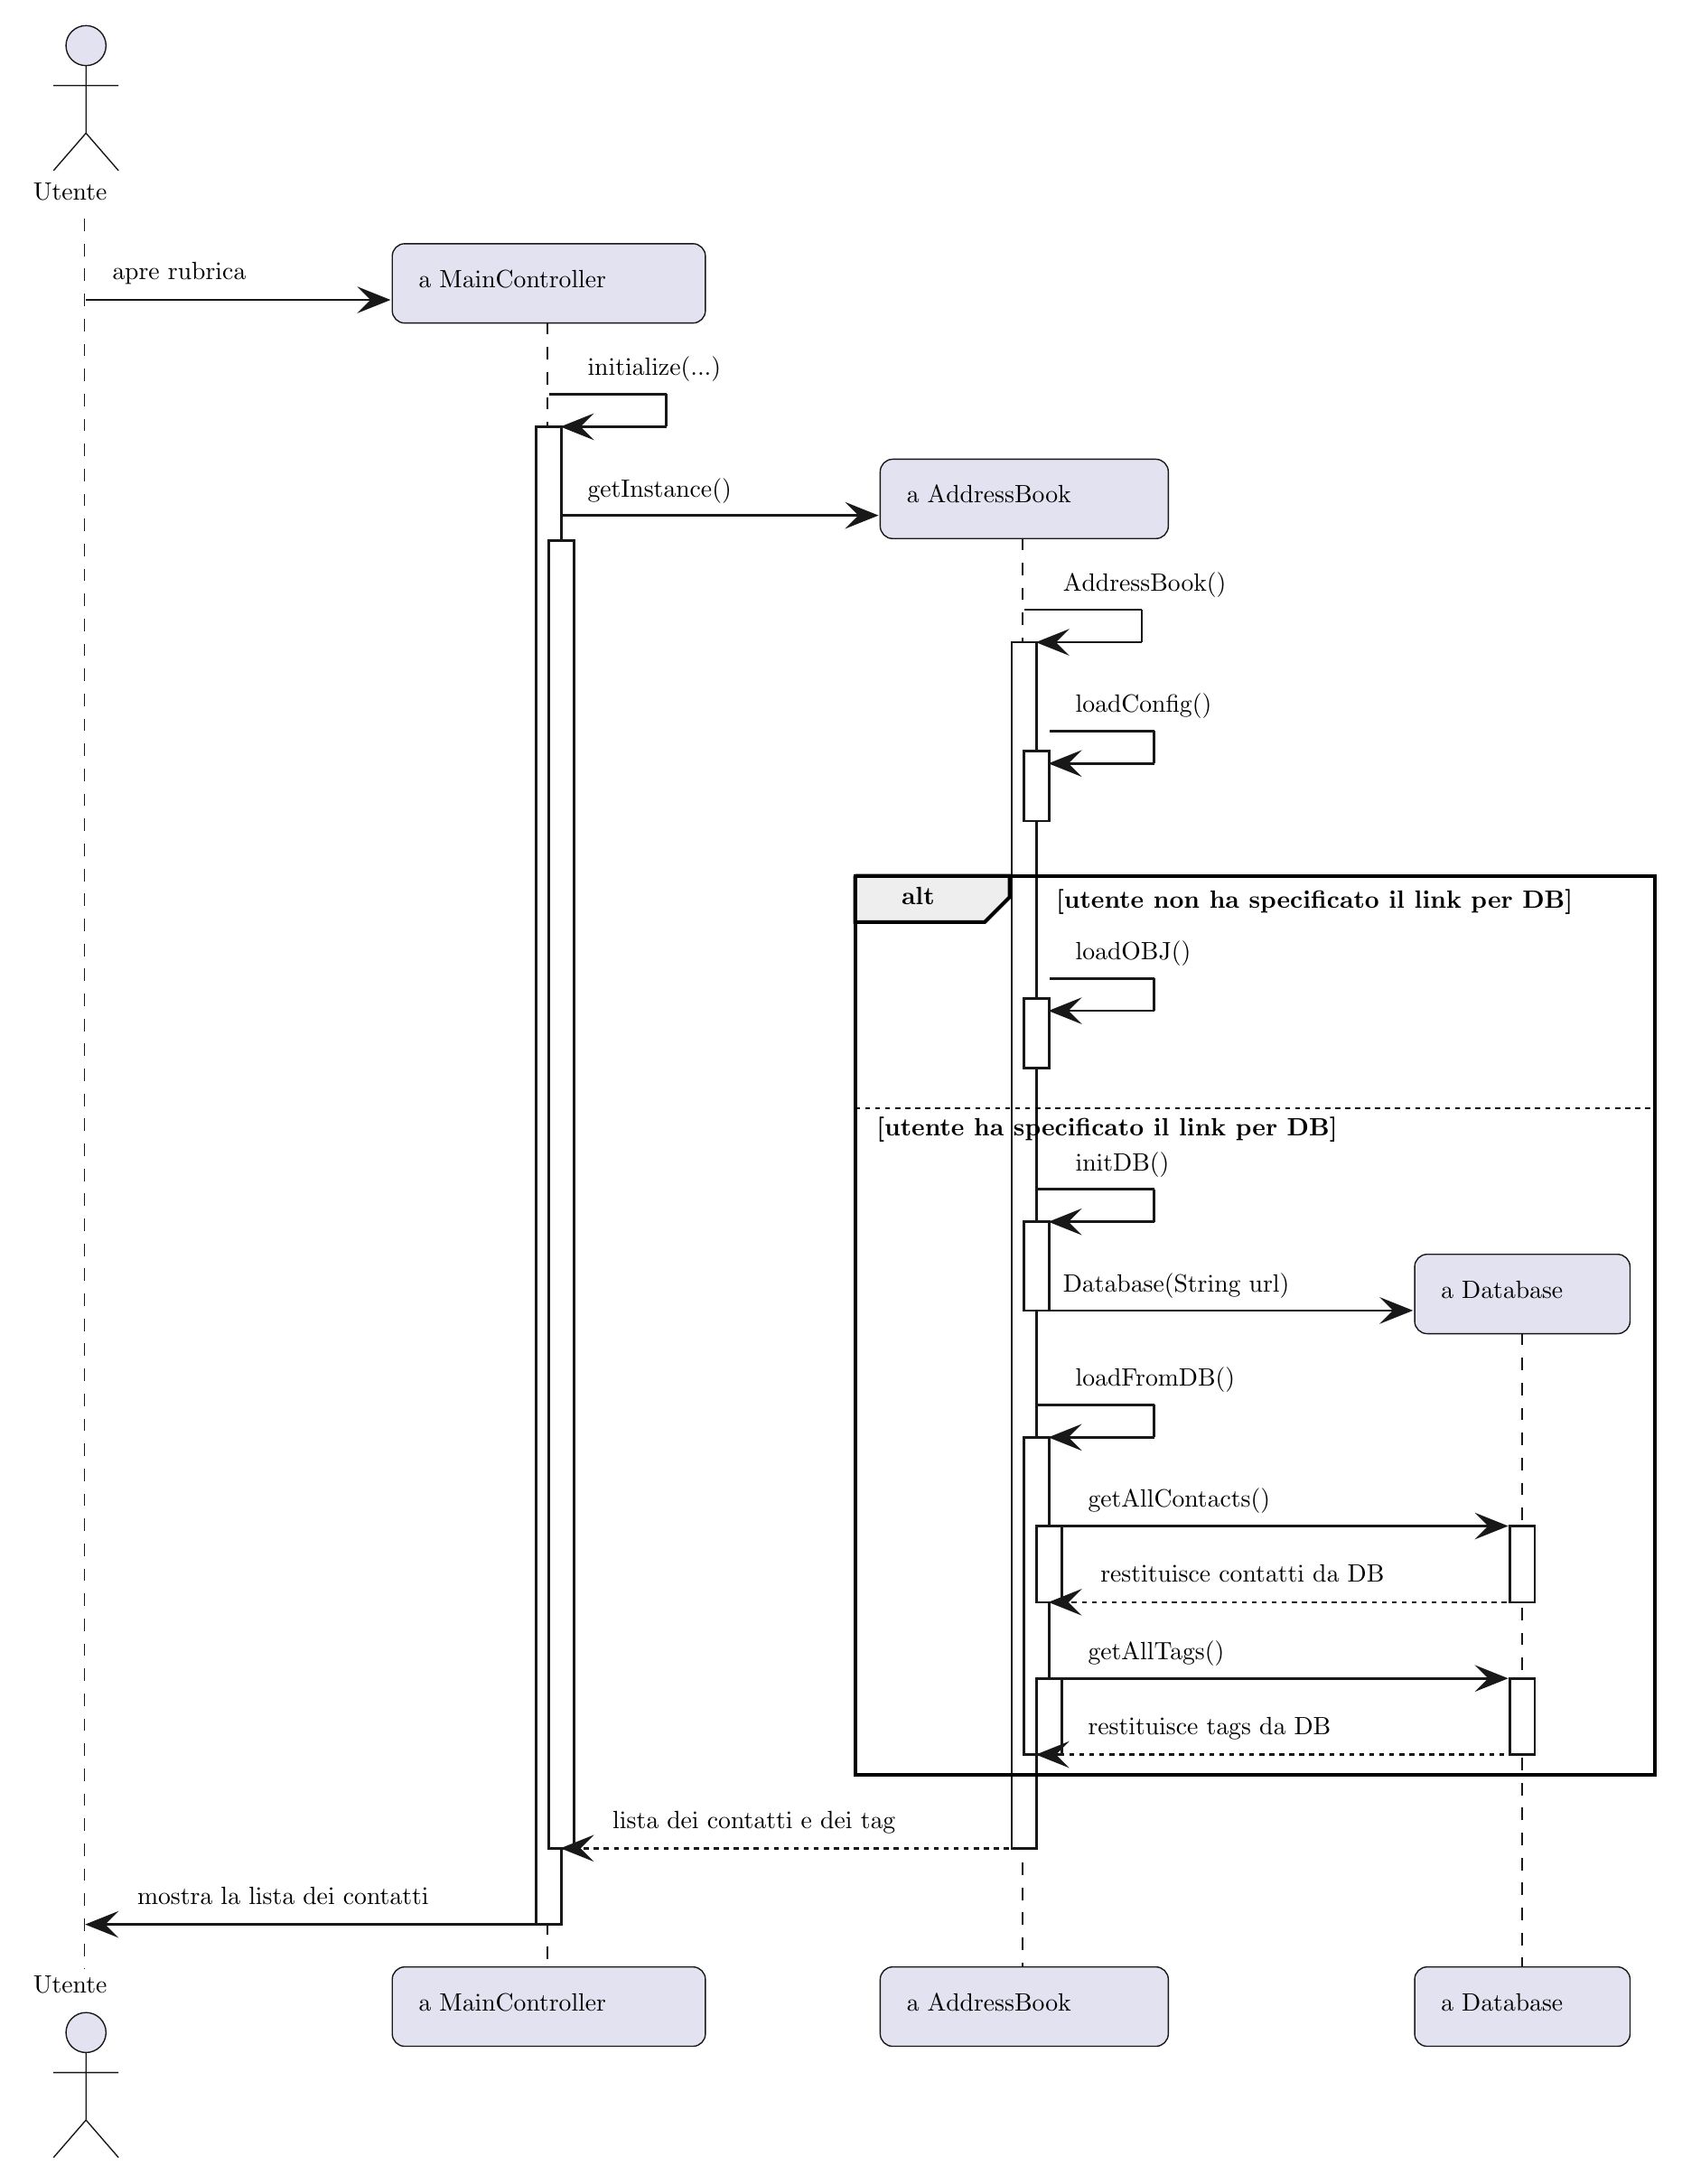
\begin{tikzpicture}[yscale=-1
,pstyle0/.style={color=plantucolor0001,fill=white,line width=1.0pt}
,pstyle1/.style={color=black,line width=1.5pt}
,pstyle2/.style={color=plantucolor0001,line width=0.5pt,dash pattern=on 5.0pt off 5.0pt}
,pstyle3/.style={color=plantucolor0001,fill=plantucolor0003,line width=0.5pt}
,pstyle4/.style={color=plantucolor0001,line width=0.5pt}
,pstyle5/.style={color=plantucolor0001,fill=plantucolor0001,line width=1.0pt}
,pstyle6/.style={color=plantucolor0001,line width=1.0pt}
,pstyle9/.style={color=plantucolor0001,line width=1.0pt,dash pattern=on 2.0pt off 2.0pt}
]
\draw[pstyle0] (209.7412pt,165.9707pt) rectangle (219.7412pt,765.1484pt);
\draw[pstyle0] (214.7412pt,211.4492pt) rectangle (224.7412pt,734.6699pt);
\draw[pstyle0] (399.9201pt,252.1953pt) rectangle (409.9201pt,734.6699pt);
\draw[pstyle0] (404.9201pt,295.6738pt) rectangle (414.9201pt,323.6738pt);
\draw[pstyle0] (404.9201pt,394.6309pt) rectangle (414.9201pt,422.6309pt);
\draw[pstyle0] (404.9201pt,484.0527pt) rectangle (414.9201pt,519.5313pt);
\draw[pstyle0] (404.9201pt,570.2773pt) rectangle (414.9201pt,697.1914pt);
\draw[pstyle0] (409.9201pt,605.7559pt) rectangle (419.9201pt,636.2344pt);
\draw[pstyle0] (409.9201pt,666.7129pt) rectangle (419.9201pt,697.1914pt);
\draw[pstyle0] (599.1646pt,605.7559pt) rectangle (609.1646pt,636.2344pt);
\draw[pstyle0] (599.1646pt,666.7129pt) rectangle (609.1646pt,697.1914pt);
\draw[pstyle1] (337.2966pt,345.6738pt) rectangle (657.24pt,705.1914pt);
\draw[pstyle2] (29pt,82.7461pt) -- (29pt,783.1484pt);
\draw[pstyle2] (214.1071pt,124.1191pt) -- (214.1071pt,783.1484pt);
\draw[pstyle2] (404.2966pt,210.3438pt) -- (404.2966pt,783.1484pt);
\draw[pstyle2] (604.0892pt,528.4258pt) -- (604.0892pt,783.1484pt);
\node at (5pt,65pt)[below right,color=black]{Utente};
\draw[pstyle3] (29.6pt,13.5pt) ellipse (8pt and 8pt);
\draw[pstyle4] (29.6pt,21.5pt) -- (29.6pt,48.5pt)(16.6pt,29.5pt) -- (42.6pt,29.5pt)(29.6pt,48.5pt) -- (16.6pt,63.5pt)(29.6pt,48.5pt) -- (42.6pt,63.5pt);
\node at (5pt,782.1484pt)[below right,color=black]{Utente};
\draw[pstyle3] (29.6pt,808.3945pt) ellipse (8pt and 8pt);
\draw[pstyle4] (29.6pt,816.3945pt) -- (29.6pt,843.3945pt)(16.6pt,824.3945pt) -- (42.6pt,824.3945pt)(29.6pt,843.3945pt) -- (16.6pt,858.3945pt)(29.6pt,843.3945pt) -- (42.6pt,858.3945pt);
\draw[pstyle3] (152.1071pt,787.1484pt) arc (180:270:5pt) -- (157.1071pt,782.1484pt) -- (272.3752pt,782.1484pt) arc (270:360:5pt) -- (277.3752pt,787.1484pt) -- (277.3752pt,808.8945pt) arc (0:90:5pt) -- (272.3752pt,813.8945pt) -- (157.1071pt,813.8945pt) arc (90:180:5pt) -- (152.1071pt,808.8945pt) -- cycle;
\node at (159.1071pt,789.1484pt)[below right,color=black]{a MainController};
\draw[pstyle3] (347.2966pt,787.1484pt) arc (180:270:5pt) -- (352.2966pt,782.1484pt) -- (457.5437pt,782.1484pt) arc (270:360:5pt) -- (462.5437pt,787.1484pt) -- (462.5437pt,808.8945pt) arc (0:90:5pt) -- (457.5437pt,813.8945pt) -- (352.2966pt,813.8945pt) arc (90:180:5pt) -- (347.2966pt,808.8945pt) -- cycle;
\node at (354.2966pt,789.1484pt)[below right,color=black]{a AddressBook};
\draw[pstyle3] (561.0892pt,787.1484pt) arc (180:270:5pt) -- (566.0892pt,782.1484pt) -- (642.24pt,782.1484pt) arc (270:360:5pt) -- (647.24pt,787.1484pt) -- (647.24pt,808.8945pt) arc (0:90:5pt) -- (642.24pt,813.8945pt) -- (566.0892pt,813.8945pt) arc (90:180:5pt) -- (561.0892pt,808.8945pt) -- cycle;
\node at (568.0892pt,789.1484pt)[below right,color=black]{a Database};
\draw[pstyle0] (209.7412pt,165.9707pt) rectangle (219.7412pt,765.1484pt);
\draw[pstyle0] (214.7412pt,211.4492pt) rectangle (224.7412pt,734.6699pt);
\draw[pstyle0] (399.9201pt,252.1953pt) rectangle (409.9201pt,734.6699pt);
\draw[pstyle0] (404.9201pt,295.6738pt) rectangle (414.9201pt,323.6738pt);
\draw[pstyle0] (404.9201pt,394.6309pt) rectangle (414.9201pt,422.6309pt);
\draw[pstyle0] (404.9201pt,484.0527pt) rectangle (414.9201pt,519.5313pt);
\draw[pstyle0] (404.9201pt,570.2773pt) rectangle (414.9201pt,697.1914pt);
\draw[pstyle0] (409.9201pt,605.7559pt) rectangle (419.9201pt,636.2344pt);
\draw[pstyle0] (409.9201pt,666.7129pt) rectangle (419.9201pt,697.1914pt);
\draw[pstyle0] (599.1646pt,605.7559pt) rectangle (609.1646pt,636.2344pt);
\draw[pstyle0] (599.1646pt,666.7129pt) rectangle (609.1646pt,697.1914pt);
\draw[pstyle5] (140.1071pt,111.2246pt) -- (150.1071pt,115.2246pt) -- (140.1071pt,119.2246pt) -- (144.1071pt,115.2246pt) -- cycle;
\draw[pstyle6] (29.6pt,115.2246pt) -- (146.1071pt,115.2246pt);
\node at (36.6pt,96.7461pt)[below right,color=black]{apre rubrica};
\draw[pstyle3] (152.1071pt,97.7461pt) arc (180:270:5pt) -- (157.1071pt,92.7461pt) -- (272.3752pt,92.7461pt) arc (270:360:5pt) -- (277.3752pt,97.7461pt) -- (277.3752pt,119.4922pt) arc (0:90:5pt) -- (272.3752pt,124.4922pt) -- (157.1071pt,124.4922pt) arc (90:180:5pt) -- (152.1071pt,119.4922pt) -- cycle;
\node at (159.1071pt,99.7461pt)[below right,color=black]{a MainController};
\draw[pstyle6] (214.7412pt,152.9707pt) -- (261.7412pt,152.9707pt);
\draw[pstyle6] (261.7412pt,152.9707pt) -- (261.7412pt,165.9707pt);
\draw[pstyle6] (220.7412pt,165.9707pt) -- (261.7412pt,165.9707pt);
\draw[pstyle5] (230.7412pt,161.9707pt) -- (220.7412pt,165.9707pt) -- (230.7412pt,169.9707pt) -- (226.7412pt,165.9707pt) -- cycle;
\node at (226.7412pt,134.4922pt)[below right,color=black]{initialize(...)};
\draw[pstyle5] (335.2966pt,197.4492pt) -- (345.2966pt,201.4492pt) -- (335.2966pt,205.4492pt) -- (339.2966pt,201.4492pt) -- cycle;
\draw[pstyle6] (219.7412pt,201.4492pt) -- (341.2966pt,201.4492pt);
\node at (226.7412pt,182.9707pt)[below right,color=black]{getInstance()};
\draw[pstyle3] (347.2966pt,183.9707pt) arc (180:270:5pt) -- (352.2966pt,178.9707pt) -- (457.5437pt,178.9707pt) arc (270:360:5pt) -- (462.5437pt,183.9707pt) -- (462.5437pt,205.7168pt) arc (0:90:5pt) -- (457.5437pt,210.7168pt) -- (352.2966pt,210.7168pt) arc (90:180:5pt) -- (347.2966pt,205.7168pt) -- cycle;
\node at (354.2966pt,185.9707pt)[below right,color=black]{a AddressBook};
\draw[pstyle6] (404.9201pt,239.1953pt) -- (451.9201pt,239.1953pt);
\draw[pstyle6] (451.9201pt,239.1953pt) -- (451.9201pt,252.1953pt);
\draw[pstyle6] (410.9201pt,252.1953pt) -- (451.9201pt,252.1953pt);
\draw[pstyle5] (420.9201pt,248.1953pt) -- (410.9201pt,252.1953pt) -- (420.9201pt,256.1953pt) -- (416.9201pt,252.1953pt) -- cycle;
\node at (416.9201pt,220.7168pt)[below right,color=black]{AddressBook()};
\draw[pstyle6] (414.9201pt,287.6738pt) -- (456.9201pt,287.6738pt);
\draw[pstyle6] (456.9201pt,287.6738pt) -- (456.9201pt,300.6738pt);
\draw[pstyle6] (415.9201pt,300.6738pt) -- (456.9201pt,300.6738pt);
\draw[pstyle5] (425.9201pt,296.6738pt) -- (415.9201pt,300.6738pt) -- (425.9201pt,304.6738pt) -- (421.9201pt,300.6738pt) -- cycle;
\node at (421.9201pt,269.1953pt)[below right,color=black]{loadConfig()};
\draw[color=black,fill=plantucolor0004,line width=1.5pt] (337.2966pt,345.6738pt) -- (399.0966pt,345.6738pt) -- (399.0966pt,354.1523pt) -- (389.0966pt,364.1523pt) -- (337.2966pt,364.1523pt) -- (337.2966pt,345.6738pt);
\draw[pstyle1] (337.2966pt,345.6738pt) rectangle (657.24pt,705.1914pt);
\node at (352.2966pt,346.6738pt)[below right,color=black]{\textbf{alt}};
\node at (414.0966pt,347.6738pt)[below right,color=black]{\textbf{[utente non ha specificato il link per DB]}};
\draw[pstyle6] (414.9201pt,386.6309pt) -- (456.9201pt,386.6309pt);
\draw[pstyle6] (456.9201pt,386.6309pt) -- (456.9201pt,399.6309pt);
\draw[pstyle6] (415.9201pt,399.6309pt) -- (456.9201pt,399.6309pt);
\draw[pstyle5] (425.9201pt,395.6309pt) -- (415.9201pt,399.6309pt) -- (425.9201pt,403.6309pt) -- (421.9201pt,399.6309pt) -- cycle;
\node at (421.9201pt,368.1523pt)[below right,color=black]{loadOBJ()};
\draw[color=black,line width=1.0pt,dash pattern=on 2.0pt off 2.0pt] (337.2966pt,438.6309pt) -- (657.24pt,438.6309pt);
\node at (342.2966pt,438.6309pt)[below right,color=black]{\textbf{[utente ha specificato il link per DB]}};
\draw[pstyle6] (409.9201pt,471.0527pt) -- (456.9201pt,471.0527pt);
\draw[pstyle6] (456.9201pt,471.0527pt) -- (456.9201pt,484.0527pt);
\draw[pstyle6] (415.9201pt,484.0527pt) -- (456.9201pt,484.0527pt);
\draw[pstyle5] (425.9201pt,480.0527pt) -- (415.9201pt,484.0527pt) -- (425.9201pt,488.0527pt) -- (421.9201pt,484.0527pt) -- cycle;
\node at (421.9201pt,452.5742pt)[below right,color=black]{initDB()};
\draw[pstyle5] (549.0892pt,515.5313pt) -- (559.0892pt,519.5313pt) -- (549.0892pt,523.5313pt) -- (553.0892pt,519.5313pt) -- cycle;
\draw[pstyle6] (409.9201pt,519.5313pt) -- (555.0892pt,519.5313pt);
\node at (416.9201pt,501.0527pt)[below right,color=black]{Database(String url)};
\draw[pstyle3] (561.0892pt,502.0527pt) arc (180:270:5pt) -- (566.0892pt,497.0527pt) -- (642.24pt,497.0527pt) arc (270:360:5pt) -- (647.24pt,502.0527pt) -- (647.24pt,523.7988pt) arc (0:90:5pt) -- (642.24pt,528.7988pt) -- (566.0892pt,528.7988pt) arc (90:180:5pt) -- (561.0892pt,523.7988pt) -- cycle;
\node at (568.0892pt,504.0527pt)[below right,color=black]{a Database};
\draw[pstyle6] (409.9201pt,557.2773pt) -- (456.9201pt,557.2773pt);
\draw[pstyle6] (456.9201pt,557.2773pt) -- (456.9201pt,570.2773pt);
\draw[pstyle6] (415.9201pt,570.2773pt) -- (456.9201pt,570.2773pt);
\draw[pstyle5] (425.9201pt,566.2773pt) -- (415.9201pt,570.2773pt) -- (425.9201pt,574.2773pt) -- (421.9201pt,570.2773pt) -- cycle;
\node at (421.9201pt,538.7988pt)[below right,color=black]{loadFromDB()};
\draw[pstyle5] (587.1646pt,601.7559pt) -- (597.1646pt,605.7559pt) -- (587.1646pt,609.7559pt) -- (591.1646pt,605.7559pt) -- cycle;
\draw[pstyle6] (419.9201pt,605.7559pt) -- (593.1646pt,605.7559pt);
\node at (426.9201pt,587.2773pt)[below right,color=black]{getAllContacts()};
\draw[pstyle5] (425.9201pt,632.2344pt) -- (415.9201pt,636.2344pt) -- (425.9201pt,640.2344pt) -- (421.9201pt,636.2344pt) -- cycle;
\draw[pstyle9] (419.9201pt,636.2344pt) -- (603.1646pt,636.2344pt);
\node at (431.9201pt,617.7559pt)[below right,color=black]{restituisce contatti da DB};
\draw[pstyle5] (587.1646pt,662.7129pt) -- (597.1646pt,666.7129pt) -- (587.1646pt,670.7129pt) -- (591.1646pt,666.7129pt) -- cycle;
\draw[pstyle6] (419.9201pt,666.7129pt) -- (593.1646pt,666.7129pt);
\node at (426.9201pt,648.2344pt)[below right,color=black]{getAllTags()};
\draw[pstyle5] (420.9201pt,693.1914pt) -- (410.9201pt,697.1914pt) -- (420.9201pt,701.1914pt) -- (416.9201pt,697.1914pt) -- cycle;
\draw[pstyle9] (414.9201pt,697.1914pt) -- (603.1646pt,697.1914pt);
\node at (426.9201pt,678.7129pt)[below right,color=black]{restituisce tags da DB};
\draw[pstyle5] (230.7412pt,730.6699pt) -- (220.7412pt,734.6699pt) -- (230.7412pt,738.6699pt) -- (226.7412pt,734.6699pt) -- cycle;
\draw[pstyle9] (224.7412pt,734.6699pt) -- (403.9201pt,734.6699pt);
\node at (236.7412pt,716.1914pt)[below right,color=black]{lista dei contatti e dei tag};
\draw[pstyle5] (40.6pt,761.1484pt) -- (30.6pt,765.1484pt) -- (40.6pt,769.1484pt) -- (36.6pt,765.1484pt) -- cycle;
\draw[pstyle6] (34.6pt,765.1484pt) -- (213.7412pt,765.1484pt);
\node at (46.6pt,746.6699pt)[below right,color=black]{mostra la lista dei contatti};
\end{tikzpicture}
}
\end{adjustbox}

\begin{figure}[h]
	\caption{Diagramma sequenza Inizializzazione rubrica}
	\label{fig:Diagramma sequenza Inizializzazione rubrica}
\end{figure}


\newpage
\subsection{Principi di buona progettazione}
Si garantisce l'aderenza ai principi di buona progettazione del software, migliorando modularità, manutenibilità e chiarezza del sistema.
\subsubsection{Livelli di coesione}
\begin{figure}[h]
	\centering
	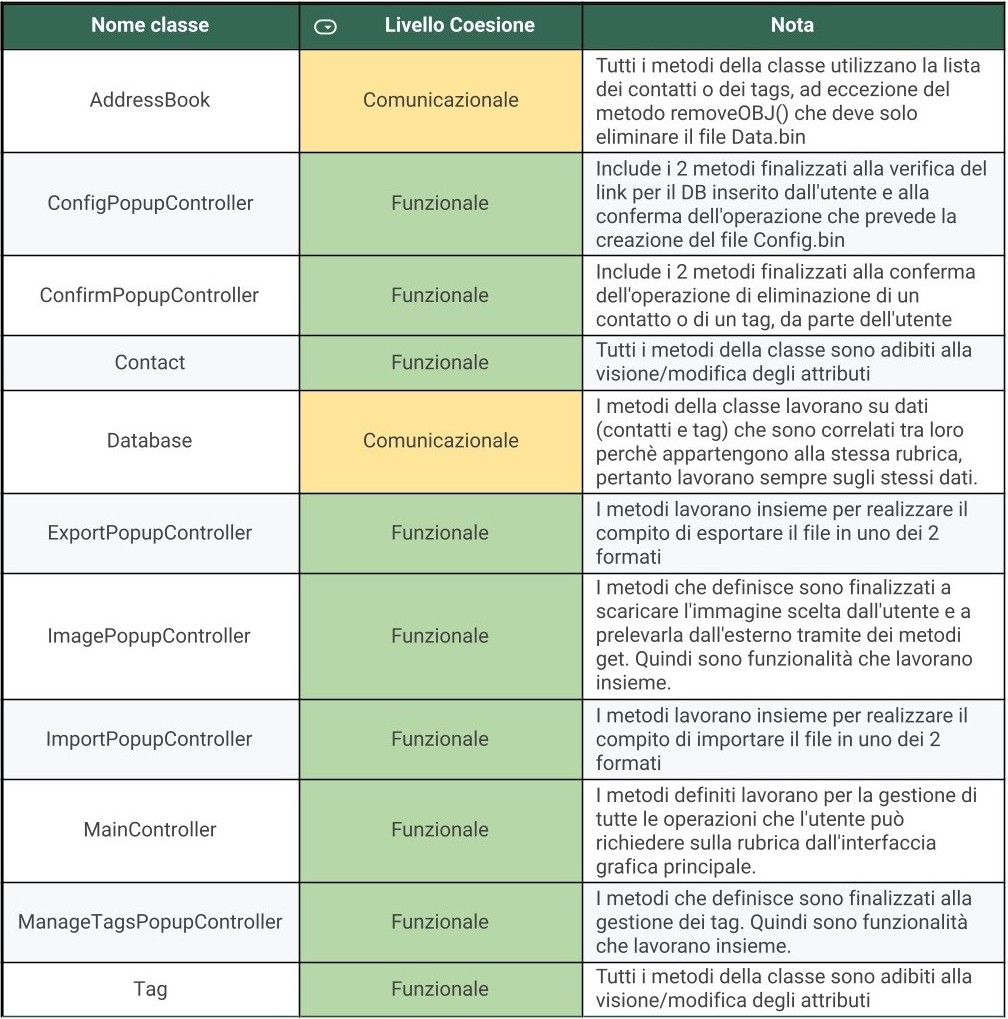
\includegraphics[width=.9\linewidth]{images/Coesione classi.jpg}
	\caption{Livelli di coesione classi}
	\label{fig:livelli di coesione classi}
\end{figure}
\newpage
\subsubsection{Livelli di accoppiamento}
\begin{figure}[h]
	\centering
	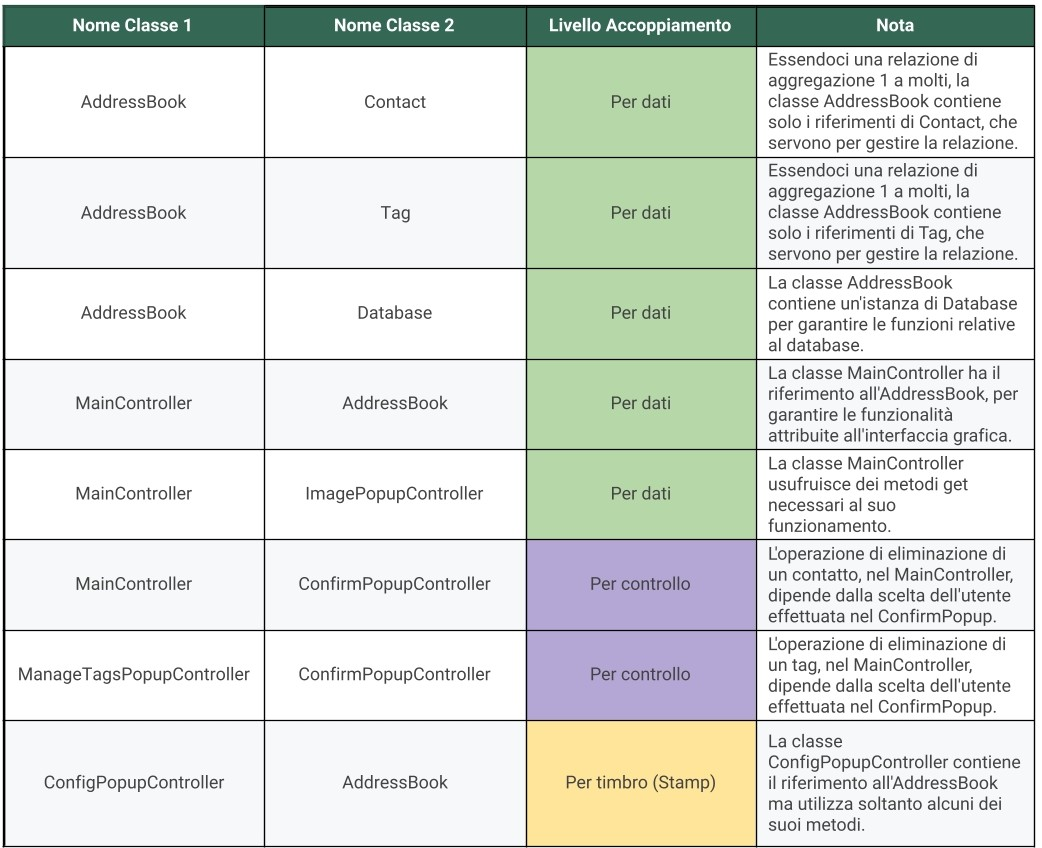
\includegraphics[width=.9\linewidth]{images/Accoppiamento_classi.jpg}
	\caption{Livelli di accoppiamento classi}
	\label{fig:livelli di accoppiamento classi}
\end{figure}

\subsubsection{Relazioni tra le Classi}
Nel progetto si è prediletta l’associazione rispetto alla specializzazione (ereditarietà). \\
In particolare:
\begin{itemize}[noitemsep, topsep=5pt]
	\item Esiste una relazione di aggregazione 1 a molti tra \textit{AddressBook} e \textit{Contact}, tra \textit{AddressBook} e \textit{Tag}.
	\item È presente una relazione di composizione 1 a 0..1 tra \textit{AddressBook} e \textit{Database}, poiché la rubrica può prevedere il salvataggio su database o in locale.
\end{itemize}

\subsubsection{Riduzione dell’Accoppiamento}
Per seguire il principio di riduzione dell’accoppiamento tra classi, sono state create le interfacce \textit{TagManager} e \textit{ContactManager}. \\
Questo consente alle classi \textit{Export}, \textit{Import} e \textit{ManageTagsPopupController} di accedere solo ai metodi strettamente necessari, favorendo anche il principio di segregazione delle interfacce.\\
Tuttavia:
\begin{itemize}[noitemsep, topsep=5pt]
	\item \textit{MainController} ha un riferimento diretto a \textit{AddressBook}, poiché dipende da esso per la maggior parte dei metodi, esclusi quelli relativi ai tag.
	\item \textit{ConfigPopupController} ha anch’esso un riferimento diretto a \textit{AddressBook}, ma con un accoppiamento per timbro, dato che utilizza solo alcuni metodi.
\end{itemize}
\subsubsection{Relazione con l’Interfaccia Initializable}
Tutti i controller implementano l’interfaccia \textit{Initializable}, ma nei diagrammi di classe tale relazione viene omessa per ridurre il livello di dettaglio e garantire una maggiore visibilità.

\subsubsection{Livelli di dettaglio}
Sono forniti due diagrammi di classi con livelli di dettaglio differenti:
\begin{itemize}[noitemsep, topsep=5pt]
	\item Diagramma con relazioni evidenziate: Mostra solo i metodi e attributi più rilevanti, evidenziando meglio le relazioni.
	\item Diagramma completo: Descrive in dettaglio tutti gli attributi e metodi delle classi, evidenziandone più concretamente il ruolo nella realizzazione del sistema.
\end{itemize}

\subsubsection{Diagrammi di Sequenza}
Sono forniti diagrammi di sequenza per descrivere i flussi di eventi relativi all’interazione tra l’utente e la rubrica, tra cui:
\begin{itemize}[noitemsep, topsep=5pt]
	\item Alcuni casi d’uso specifici (C1, C2, C3, C5, C6, C8).
	\item L’operazione di aggiunta del database tramite link inserito dall’utente.
	\item Lo scenario di apertura e inizializzazione della rubrica, che può avvenire attraverso il database o il file locale \texttt{Data.bin} in assenza del database.
\end{itemize}